\documentclass[fontsize=13pt,oneside,a4paper,openany]{kltn}

\usepackage{csquotes}
\usepackage{tabularx}
\usepackage{multirow}
\usepackage{array}
\usepackage{tabularx}
\usepackage{lmodern}
\usepackage{booktabs}

\usepackage{tikz}
\usetikzlibrary{positioning}



\usepackage{caption}

\captionsetup[figure]{name=Hình, labelsep=period}
\captionsetup[table]{name=Bảng, labelsep=period}


% Tài liệu tham khảo
\addbibresource{refs.bib}

\begin{document} 

\include{tex/00bia}  	

\VKnumRoman     % đánh số bằng chữ cái i, ii...

\include{tex/01camon}		
\include{tex/02camdoan}	
\include{tex/03tomtat}

\VKmucLuc				
\VKdanhMucHinhVe		
\VKdanhMucBangBieu		
\input{tex/04kyhieu}

\VKbatDaudanhSo     % bắt đầu đánh số từ 1,2,3...

\include{chapter/chapter0}		
\chapter{Giới thiệu chung}

% ==========================================================
\section{Tổng quan về hệ thống AVI trong công nghiệp}

Trong bối cảnh cạnh tranh sản xuất ngày càng khốc liệt, việc duy trì chất lượng sản phẩm ổn định không chỉ là lợi thế mà đã trở thành yêu cầu bắt buộc. Các lỗi ngoại quan, dù rất nhỏ, đều có thể gây ra chi phí lớn như thu hồi sản phẩm, gián đoạn dây chuyền và ảnh hưởng nghiêm trọng đến uy tín thương hiệu. Kiểm tra ngoại quan thủ công, vốn phụ thuộc nhiều vào con người, khó đảm bảo tính ổn định và tốc độ trong dây chuyền hiện đại.

Hệ thống kiểm tra ngoại quan tự động — \textit{Automated Visual Inspection} (AVI) — ra đời như một giải pháp tất yếu, tận dụng thị giác máy và trí tuệ nhân tạo để tự động phát hiện lỗi và đánh giá chất lượng theo thời gian thực. Theo dự báo, thị trường thị giác máy toàn cầu sẽ đạt khoảng \textbf{9,29 tỷ USD} vào năm 2032 với tốc độ tăng trưởng 7,2\%/năm \cite{easyodm_AVI2025}, phản ánh nhu cầu rất lớn về tự động hoá và kiểm tra chất lượng trong Công nghiệp 4.0.

\subsection*{Khái niệm và chức năng của hệ thống AVI}

AVI là hệ thống kiểm tra chất lượng dựa trên camera công nghiệp, hệ thống chiếu sáng và thuật toán xử lý ảnh. Các chức năng chính bao gồm:

\begin{itemize}
    \item Phát hiện và phân loại lỗi trên sản phẩm.
    \item Định vị lỗi và đánh giá độ nghiêm trọng.
    \item Nhận diện bất thường (\textit{anomaly detection}) trên bề mặt.
    \item Đánh giá chất lượng tổng thể và đưa ra quyết định theo thời gian thực.
\end{itemize}

Các thuật toán phổ biến trong AVI gồm có Machine Learning, Deep Learning (YOLO, CNN), phương pháp phát hiện bất thường, trích xuất đặc trưng và mô hình so khớp hình ảnh.

\subsection*{Quy trình hoạt động của hệ thống AVI}

Quy trình điển hình của một hệ thống AVI bao gồm:

\begin{enumerate}
    \item \textbf{Thu nhận hình ảnh}: camera độ phân giải cao kết hợp ánh sáng phù hợp tạo ra ảnh sắc nét.
    \item \textbf{Xử lý ảnh}: lọc nhiễu, cân bằng sáng, phân đoạn và trích xuất đặc trưng.
    \item \textbf{So sánh và phân tích}: đối chiếu với tiêu chuẩn hoặc mô hình AI đã học.
    \item \textbf{Ra quyết định}: phân loại sản phẩm đạt (OK) hoặc lỗi (NG).
    \item \textbf{Phản hồi}: truyền tín hiệu điều khiển để loại bỏ sản phẩm lỗi hoặc ghi log dữ liệu.
\end{enumerate}

\subsection*{Các loại lỗi hệ thống AVI có thể phát hiện}

AVI có khả năng phát hiện nhiều loại lỗi ngoại quan:

\begin{itemize}
    \item \textbf{Lỗi bề mặt}: trầy xước, móp, đổi màu, nứt, ba via.
    \item \textbf{Lỗi kích thước}: sai lệch hình dạng, thể tích, vị trí.
    \item \textbf{Lỗi lắp ráp}: thiếu linh kiện, sai vị trí, lỗi hàn.
    \item \textbf{Lỗi bao bì}: nhãn sai, seal lỗi, mức đầy không đúng.
    \item \textbf{Lỗi vật liệu}: tạp chất, lẫn bụi, rỗ khí.
\end{itemize}


% ==========================================================
\section{Kiến trúc và thành phần của hệ thống AVI}

Một hệ thống AVI hoàn chỉnh được xây dựng từ sự kết hợp của phần cứng chuyên dụng và phần mềm xử lý mạnh mẽ nhằm đảm bảo tốc độ và độ chính xác kiểm tra.

\subsection*{Thành phần phần cứng}

\begin{itemize}
    \item \textbf{Camera công nghiệp}: area-scan, line-scan, camera 3D, multispectral, hoặc X-ray tùy ứng dụng.
    \item \textbf{Hệ thống chiếu sáng}: ring light, dome light, backlight, directional lighting, nhằm làm nổi bật đặc trưng bề mặt.
    \item \textbf{Ống kính và quang học}: lens tiêu chuẩn hoặc telecentric cho bài toán đo kích thước chính xác cao.
    \item \textbf{Cảm biến hỗ trợ}: cảm biến 3D, cảm biến tiệm cận, IR hoặc LIDAR giúp bổ sung thông tin ngoài hình ảnh.
    \item \textbf{Máy tính xử lý}: CPU/GPU hiệu năng cao để chạy các mô hình AI và xử lý ảnh thời gian thực.
\end{itemize}

\subsection*{Thành phần phần mềm}

\begin{itemize}
    \item \textbf{Xử lý ảnh}: bao gồm tiền xử lý, lọc nhiễu, phân đoạn, trích xuất đặc trưng.
    \item \textbf{AI và học máy}: YOLO, CNN, anomaly detection dùng để phát hiện lỗi phức tạp.
    \item \textbf{Giao diện người dùng (UI)}: hiển thị ảnh, kết quả kiểm tra và thống kê.
    \item \textbf{Kết nối mạng}: Ethernet/IP, OPC UA, MQTT để tích hợp vào dây chuyền.
    \item \textbf{Lưu trữ dữ liệu}: lưu ảnh kiểm tra, log sự kiện và thông số phục vụ phân tích chất lượng.
\end{itemize}


% ==========================================================
\section{Ứng dụng, lợi ích, thách thức và xu hướng phát triển}

\subsection*{Ứng dụng của AVI trong công nghiệp}

\begin{itemize}
    \item \textbf{Ô tô}: kiểm tra sơn, mối hàn, lắp ráp linh kiện.
    \item \textbf{Điện tử}: phát hiện lỗi PCB, kiểm tra mạch SMT, linh kiện thiếu hoặc sai loại.
    \item \textbf{Dược phẩm}: kiểm tra bao bì, nhãn, dị vật.
    \item \textbf{Thực phẩm}: kiểm tra mức đầy, lỗi bao bì, dị vật.
    \item \textbf{Gỗ, dệt may, bán dẫn, hàng không}: phát hiện lỗi bề mặt, nứt, sai kích thước.
\end{itemize}

\subsection*{Lợi ích nổi bật}

\begin{itemize}
    \item Độ chính xác cao (95--99,5\%), ổn định hơn kiểm tra thủ công.
    \item Tốc độ xử lý nhanh (0,1–0,5 giây/sản phẩm), vận hành 24/7.
    \item Giảm chi phí nhân lực, giảm phế phẩm, thời gian hoàn vốn ngắn (12--24 tháng).
    \item Nâng cao chất lượng đầu ra và tính nhất quán.
    \item Tích hợp linh hoạt vào dây chuyền, dễ mở rộng.
\end{itemize}

\subsection*{Thách thức và hạn chế}

\begin{itemize}
    \item Chi phí đầu tư ban đầu tương đối cao.
    \item Nhạy cảm với ánh sáng và vị trí sản phẩm.
    \item Khó phát hiện lỗi cực nhỏ nếu không có giải pháp ánh sáng phù hợp.
    \item Hệ thống AI yêu cầu dữ liệu huấn luyện đa dạng.
    \item Tích hợp vào dây chuyền hiện tại đôi khi phức tạp.
\end{itemize}

\subsection*{Xu hướng phát triển}

\begin{itemize}
    \item Tích hợp AI nâng cao và mô hình tự học.
    \item Hình ảnh 3D, hyperspectral, X-ray cho khả năng phân tích sâu hơn.
    \item Edge computing giúp xử lý thời gian thực với độ trễ thấp.
    \item Robot cộng tác và thị giác máy kết hợp cho kiểm tra linh hoạt đa góc.
    \item Hệ thống no-code cho phép kỹ thuật viên cấu hình nhanh mà không cần lập trình.
\end{itemize}

\subsection*{Kết luận}

AVI đang trở thành một thành phần không thể thiếu trong các dây chuyền sản xuất hiện đại, giúp doanh nghiệp nâng cao chất lượng sản phẩm, tối ưu chi phí và duy trì lợi thế cạnh tranh. Sự phát triển mạnh mẽ của AI và thị giác máy dự báo rằng vai trò của AVI sẽ ngày càng quan trọng trong tương lai của sản xuất thông minh.

\chapter{Cơ sở lý thuyết}
% =======================
% PHẦN 1: LÝ THUYẾT VỀ PLC VÀ HMI
% =======================
\section{PLC Mitsubishi và HMI PFXGP4501TAA}

\subsection{PLC Mitsubishi Q13UDVCPU}

Bộ điều khiển logic khả trình (PLC) Mitsubishi Q13UDVCPU (Hình \ref{c2:plc_q13udvcpu}) thuộc dòng MELSEC-Q Series, là CPU đa năng có hiệu suất xử lý cao và khả năng mở rộng linh hoạt. Với tốc độ thực thi lệnh cơ bản 1,9~ns, dung lượng chương trình 130K~steps và khả năng quản lý tới 8.192 điểm I/O, Q13UDVCPU đáp ứng tốt các yêu cầu của các dây chuyền sản xuất hiện đại, nơi cần xử lý nhanh, ổn định và có độ tin cậy cao \cite{mitsubishi_q13udvcpu}.

CPU tích hợp sẵn các giao tiếp Ethernet, USB và khe cắm thẻ SD, cho phép kết nối thuận tiện với thiết bị ngoại vi, mạng công nghiệp hoặc hệ thống SCADA. Nhờ khả năng mở rộng mạnh mẽ, Q13UDVCPU được sử dụng rộng rãi trong tự động hóa công nghiệp, đặc biệt khi kết hợp với HMI để giám sát và vận hành hệ thống.

\begin{figure}[h]
    \centering
    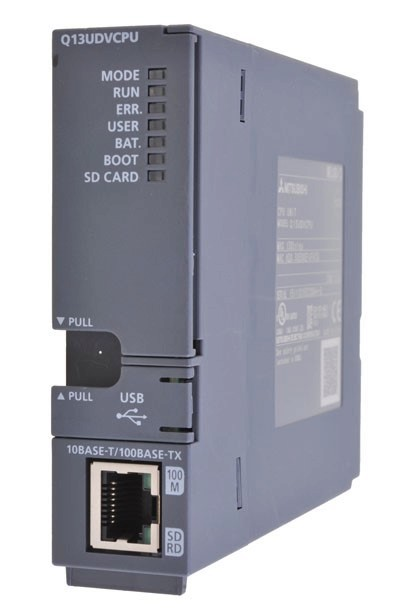
\includegraphics[width=0.33\textwidth]{figures/Chapter2/plc-cpu.png}
    \caption{CPU Mitsubishi Q13UDVCPU}
    \label{c2:plc_q13udvcpu}
\end{figure}

Một hệ thống PLC Mitsubishi Q Series cơ bản (Hình \ref{c2:plc-structure}) bao gồm các thành phần: module nguồn (Power Supply), khung base unit, CPU Q13UDVCPU và các module mở rộng I/O hoặc truyền thông. Module nguồn được lắp tại vị trí ngoài cùng bên trái nhằm cấp điện cho toàn bộ rack. CPU Q13UDVCPU được gắn trực tiếp lên base unit, tiếp theo là các module mở rộng như I/O số, I/O tương tự, module truyền thông (ví dụ CC-Link) hoặc module điều khiển chuyển động (motion).

Việc lắp đặt cần đảm bảo các đầu nối tiếp xúc chắc chắn, hạn chế bụi bẩn và rung động để đảm bảo độ ổn định của hệ thống. Sau khi hoàn tất phần cứng, PLC được cấu hình trên phần mềm GX Works2 hoặc GX Developer. Quá trình cấu hình bao gồm khai báo CPU, module nguồn, các module I/O đúng theo vị trí lắp thực tế. Nếu hệ thống sử dụng remote rack, địa chỉ truyền thông cũng cần được thiết lập tương ứng. Cấu hình chính xác giúp hệ thống hoạt động ổn định và tránh lỗi khi chạy chương trình điều khiển.

\begin{figure}[h]
    \centering
    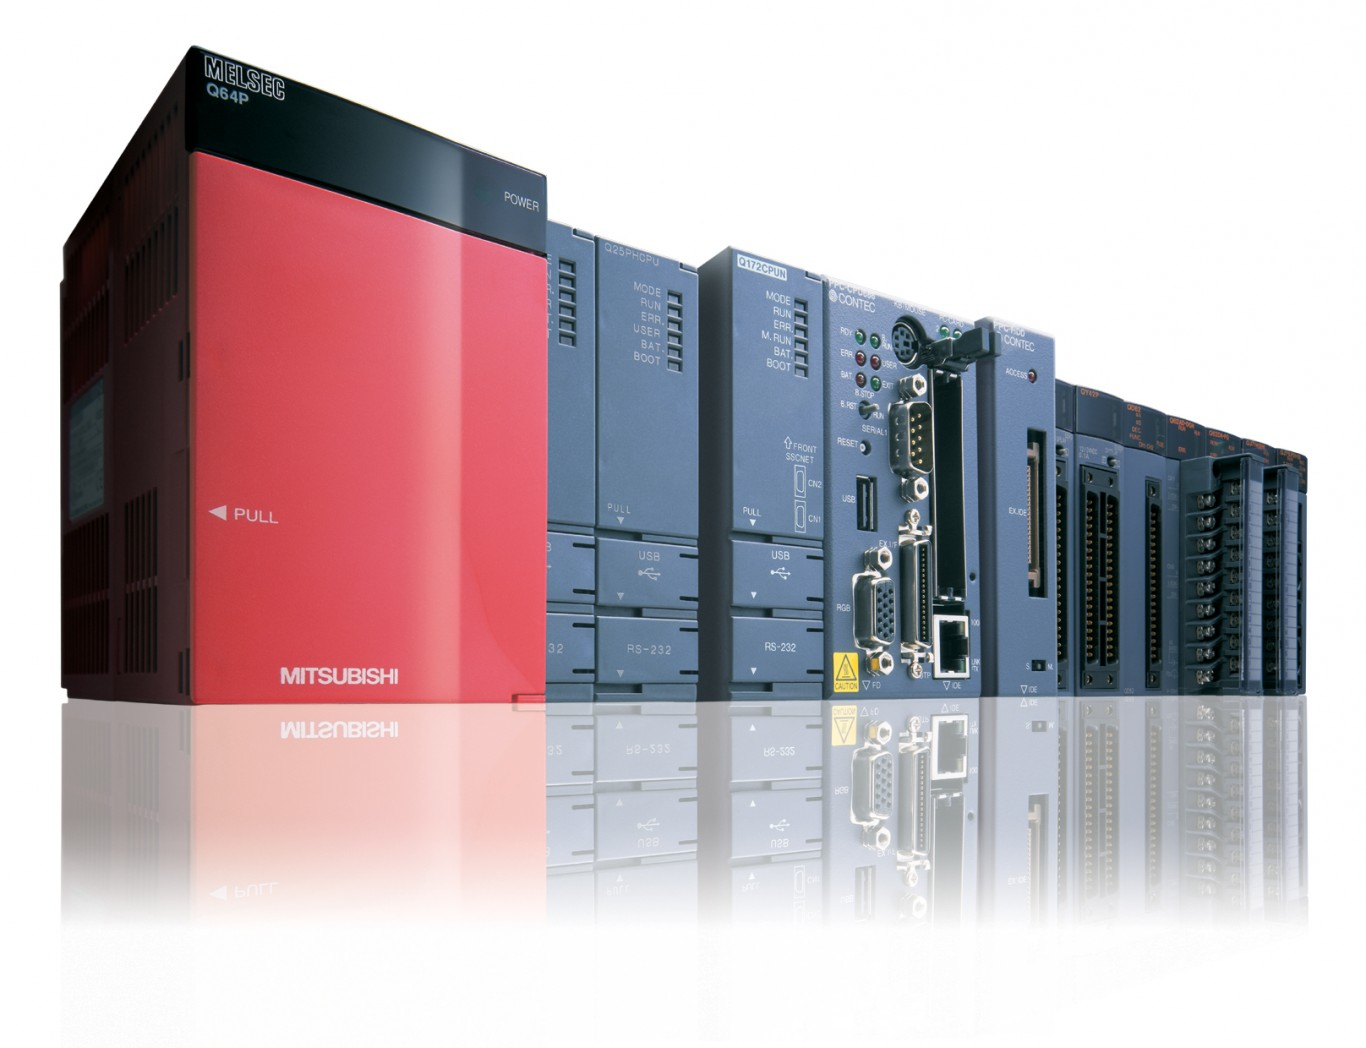
\includegraphics[width=0.75\linewidth]{figures/Chapter2/plc-structure.png}
    \caption{Hệ thống PLC Mitsubishi Q Series}
    \label{c2:plc-structure}
\end{figure}
\begin{table}[h]
\centering
\caption{Thông số kỹ thuật của PLC Mitsubishi Q13UDVCPU}
\label{tab:q13udvcpu_specs}
\begin{tabularx}{\textwidth}{|X|X|}
\hline
\textbf{Thông số} & \textbf{Giá trị} \\ \hline
Tốc độ xử lý lệnh (LD) & 1,9 ns \\ \hline
Dung lượng chương trình & 130K steps (520 kB) \\ \hline
Bộ nhớ RAM tích hợp & 1.024 kB \\ \hline
Thẻ nhớ hỗ trợ & SD/SDHC tối đa 32 GB \\ \hline
I/O tối đa (cục bộ) & 4.096 điểm \\ \hline
I/O tối đa (toàn hệ thống) & 8.192 điểm \\ \hline
Giao tiếp tích hợp & Ethernet 10/100 Mbps, USB \\ \hline
Nguồn tiêu thụ nội bộ & 0,58 A \\ \hline
Kích thước & 98 × 27,4 × 115 mm \\ \hline
Khối lượng & 0,20 kg \\ \hline
Nhiệt độ làm việc & 0 … 55 °C \\ \hline
Độ ẩm làm việc & 5 … 95\% RH (không ngưng tụ) \\ \hline
Chuẩn chống rung/sốc & JIS B 3502, IEC 61131-2 \\ \hline
\end{tabularx}
\end{table}

Phần mềm lập trình và cấu hình phổ biến cho PLC Mitsubishi Q13UDVCPU là GX Works2 \cite{gxworks2_simpleproject_manual}. Đây là môi trường phát triển tích hợp (IDE) hỗ trợ các ngôn ngữ lập trình IEC~61131-3 như Ladder Diagram (LD), Structured Text (ST) và Function Block Diagram (FBD)\cite{mitsubishi_plc_ladder_manual}. Trong GX Works2, người dùng tiến hành khai báo CPU, module nguồn, module I/O, module truyền thông hoặc motion theo đúng vị trí vật lý trên base unit. Phần mềm cũng hỗ trợ thiết lập tham số mạng (Ethernet, CC-Link), quản lý bộ nhớ, tải/chỉnh sửa chương trình qua USB hoặc Ethernet, và chức năng giám sát trạng thái online theo thời gian thực, hỗ trợ hiệu quả cho quá trình kiểm tra và gỡ lỗi.

\subsection{Giao diện người–máy HMI PFXGP4501TAA}

Giao diện Người–Máy (Human–Machine Interface, HMI) là thiết bị cho phép người vận hành tương tác trực tiếp với hệ thống điều khiển thông qua màn hình trực quan. Trong hệ thống này, HMI đảm nhiệm vai trò giám sát trạng thái, hiển thị dữ liệu sản xuất, cảnh báo lỗi và nhận lệnh vận hành từ người dùng, giúp đơn giản hóa quá trình điều khiển và giảm thiểu sai sót.

Màn hình HMI PFXGP4501TAA thuộc dòng GP4000 Series của hãng Pro-face (Schneider Electric), là thiết bị giao diện phổ biến nhờ thiết kế chắc chắn, độ ổn định cao và khả năng kết nối tốt với PLC Mitsubishi Q Series (Hình \ref{c2:hmi}).

Thiết bị được cấu hình bằng phần mềm GP-Pro EX, cho phép thiết kế giao diện, thiết lập truyền thông với PLC và xây dựng các màn hình giám sát một cách linh hoạt. Nhờ hỗ trợ nhiều giao thức công nghiệp và khả năng trực quan hóa dữ liệu tốt, HMI PFXGP4501TAA đóng vai trò quan trọng trong việc nâng cao hiệu quả vận hành và giám sát dây chuyền tự động hóa.

\begin{figure}[h]
    \centering
    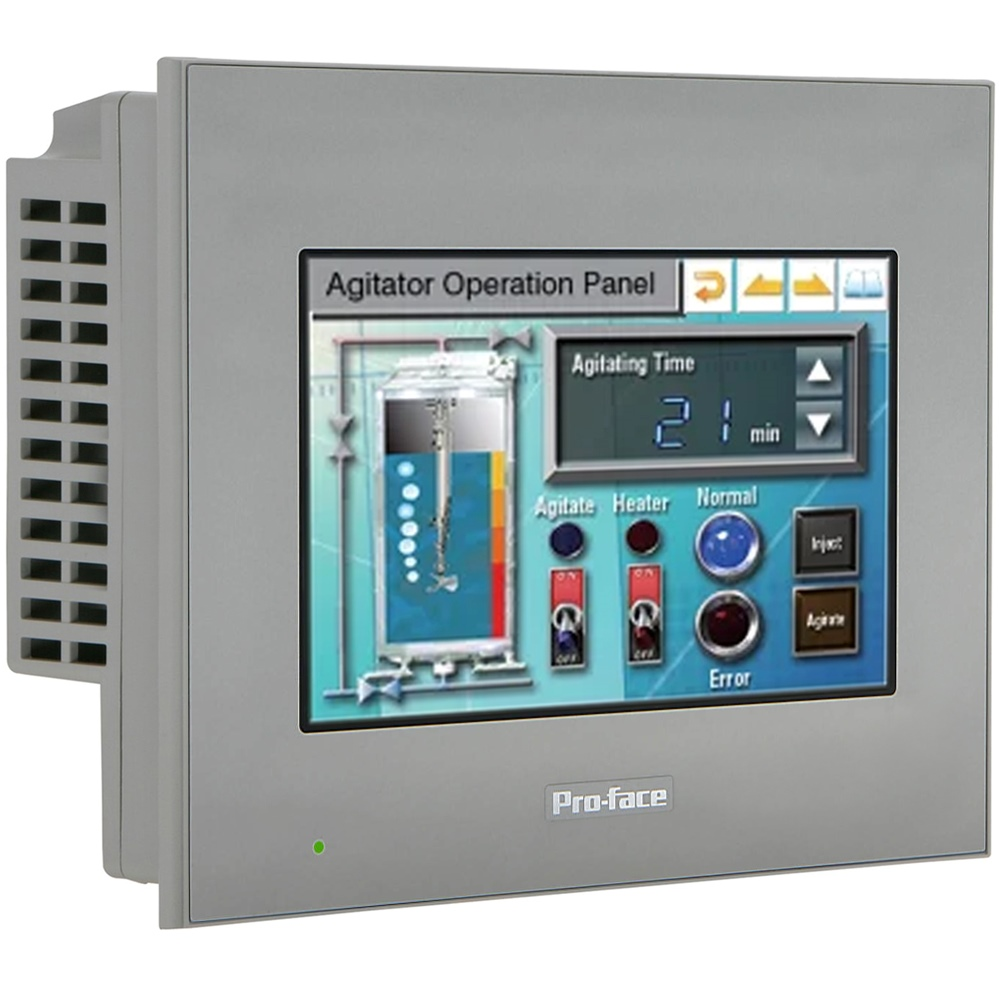
\includegraphics[width=0.43\textwidth]{figures/Chapter2/pfxgp4501taa.jpg}
    \caption{Màn hình HMI Pro-face PFXGP4501TAA}
    \label{c2:hmi}
\end{figure}

\begin{table}[h]
\centering
\caption{Thông số kỹ thuật của HMI PFXGP4501TAA}
\label{tab:hmi_specs}
\begin{tabular}{|l|l|}
\hline
\textbf{Thông số} & \textbf{Giá trị} \\ \hline
Kích thước màn hình & 10,4 inch TFT LCD \\ \hline
Độ phân giải & 640 × 480 (VGA) \\ \hline
Màu hiển thị & 65.536 màu \\ \hline
Độ sáng & 300 cd/m\textsuperscript{2} \\ \hline
Cổng giao tiếp & Ethernet, USB (Host/Device), Serial (RS-232C/422/485) \\ \hline
Bộ nhớ ứng dụng & 16 MB (Flash) \\ \hline
Nguồn cấp & 24 VDC \\ \hline
Nhiệt độ hoạt động & 0 … 50 °C \\ \hline
Kích thước ngoài & 271 × 213 × 56 mm \\ \hline
Trọng lượng & Khoảng 2,2 kg \\ \hline
Chuẩn bảo vệ & IP65 (mặt trước) \\ \hline
\end{tabular}
\end{table}



% =======================
% PHẦN 2: GIỚI THIỆU VỀ CC-LINK
% =======================
\section{Mạng CC-Link và Module CC-Link QJ61BT11N}

%===============================================================================================================
\subsection{CC-Link}

CC-Link (Control \& Communication Link) là một mạng truyền thông công nghiệp do Mitsubishi Electric phát triển, được sử dụng rộng rãi trong các hệ thống tự động hóa để kết nối PLC với các thiết bị phân tán \cite{mitsubishi_qj61bt11n_manual}. CC-Link hỗ trợ truyền cả tín hiệu ON/OFF và dữ liệu số thông qua cáp chuyên dụng, đảm bảo tốc độ cao, tính ổn định và độ tin cậy lớn trong vận hành.

Một số ưu điểm chính của CC-Link gồm:
\begin{itemize}
    \item Giảm chi phí và công sức đi dây nhờ khả năng phân tán module tại các vị trí gần thiết bị (băng chuyền, máy công cụ, robot).
    \item Hỗ trợ truyền nhận tín hiệu I/O và dữ liệu số với tốc độ cao, giảm thiểu độ trễ trong điều khiển.
    \item Cho phép nhiều PLC vận hành như các trạm phân tán trong cùng hệ thống.
    \item Tương thích với nhiều thiết bị từ các hãng đối tác trong CC-Link Partner Association (CLPA).
\end{itemize}

\begin{figure}[h]
    \centering
    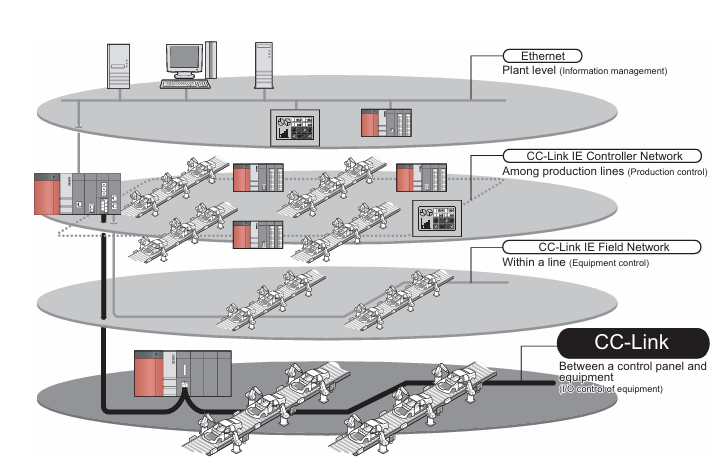
\includegraphics[width=0.7\textwidth]{figures/Chapter2/cc-link2.png}
    \caption{Cấu trúc mạng CC-Link}
    \label{fig:cclink_structure}
\end{figure}

%==============================================================================================================================
\subsection{Master/Local Modules}

Dòng PLC MELSEC-Q có thể giao tiếp với nhau hoặc với các thiết bị ngoại vi thông qua CC-Link nhờ các module Master/Local. Các trạm PLC trong mạng có thể được điều khiển như đang nằm trên cùng một base unit.

Các tính năng chính của hệ thống CC-Link:

\begin{enumerate}
    % ------------------- 1 -------------------
    \item \textbf{Truyền thông dữ liệu chu kỳ và truyền thông tức thời}  
    Master/Local Modules có thể trao đổi dữ liệu theo hai phương thức:
    \begin{itemize}
        \item \textit{Cyclic Transmission}: truyền liên tục theo chu kỳ quét của PLC.
        \item \textit{Transient Transmission}: chỉ truyền khi có yêu cầu.
    \end{itemize}

 \begin{figure}[h]
    \centering
    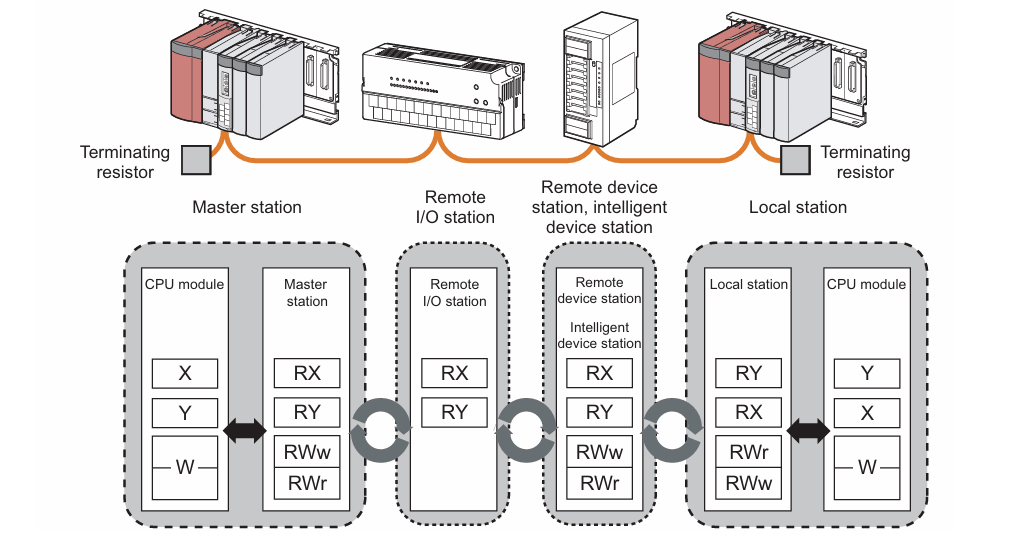
\includegraphics[width=0.48\textwidth]{figures/Chapter01/cclink3.png}
    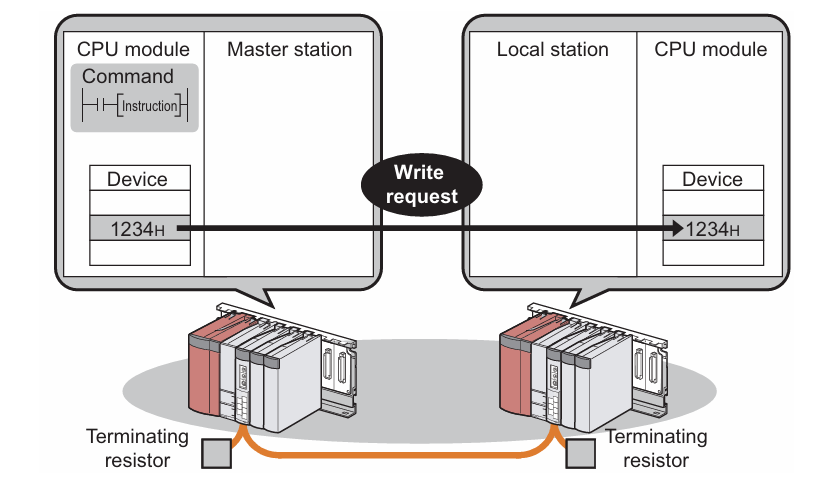
\includegraphics[width=0.48\textwidth]{figures/Chapter01/cclink4.png}
    \caption{Cyclic Transmission và Transient Transmission trong CC-Link}
    \label{fig:cclink_two}
\end{figure}


    % ------------------- 2 -------------------
    \item \textbf{Thiết lập tham số và chẩn đoán hệ thống}  
    Các tham số của module có thể được thiết lập bằng phần mềm GX Works2 hoặc bằng chính chương trình PLC. Khi thiết lập tham số từ chương trình PLC, có thể thay đổi cấu hình mà không cần reset CPU (Hình \ref{fig:cclink_config}).  
    Trạng thái hệ thống, vị trí lỗi và nguyên nhân lỗi có thể được quan sát trực tiếp trên phần mềm lập trình (Hình \ref{fig:cclink_config}).

    \begin{figure}[h]
        \centering
        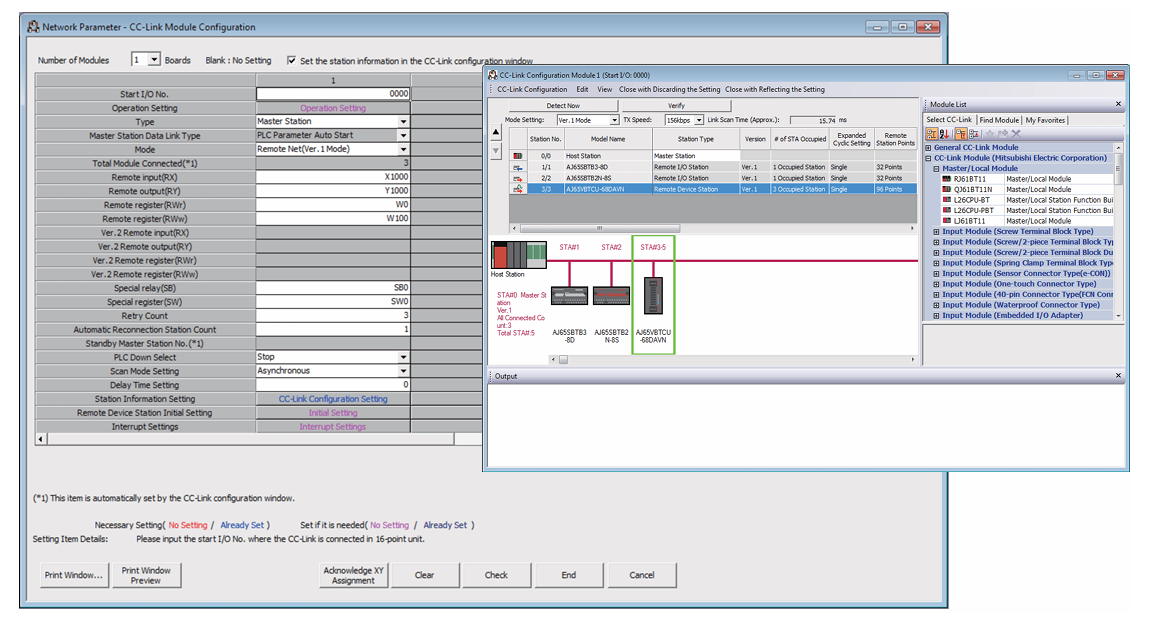
\includegraphics[width=0.48\textwidth]{figures/Chapter01/cclink5.png}
        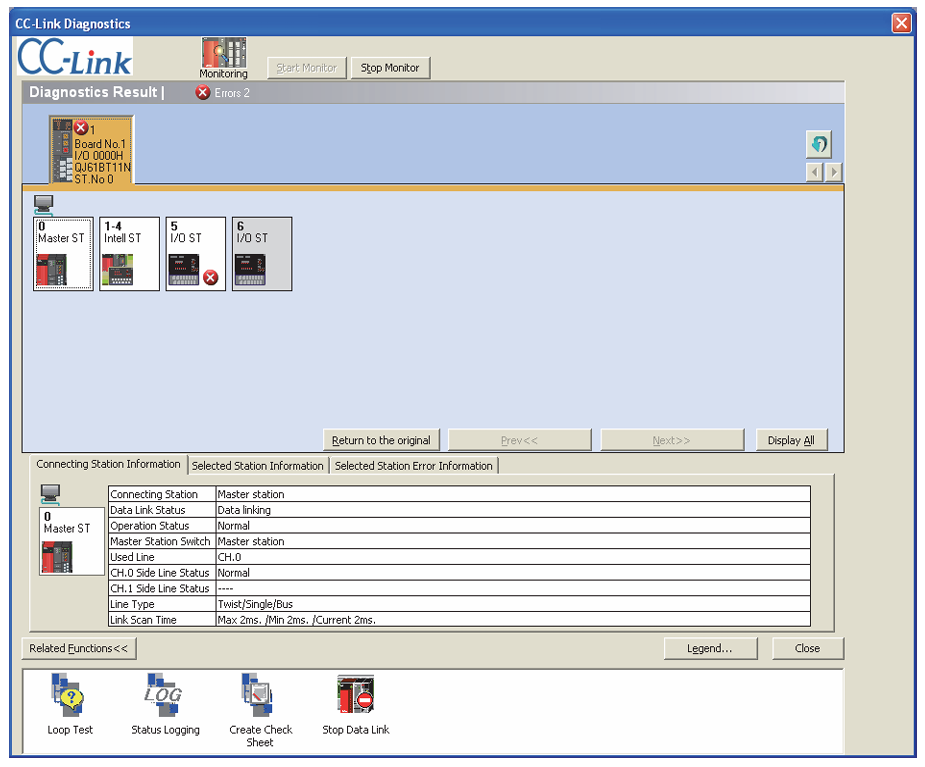
\includegraphics[width=0.48\textwidth]{figures/Chapter01/cclink6.png}
        \caption{Thiết lập tham số module CC-Link}
        \label{fig:cclink_config}
    \end{figure}


    % ------------------- 3 -------------------
    \item \textbf{Hỗ trợ CC-Link Ver.2}  
    Vì Master/Local Module hỗ trợ CC-Link Ver.2, số điểm I/O tối đa trong toàn hệ thống có thể tăng lên:
    \begin{itemize}
        \item 8192 điểm RX/RY,
        \item 2048 word RWr/RWw,
    \end{itemize}
    và theo từng trạm có thể đạt:
    \begin{itemize}
        \item 896 điểm RX/RY,
        \item 128 word RWr/RWw.
    \end{itemize}

    CC-Link Ver.2 có khả năng mở rộng lớn hơn đáng kể so với Ver.1 (Hình \ref{fig:cclink_ver2}).

    \begin{figure}[h]
        \centering
        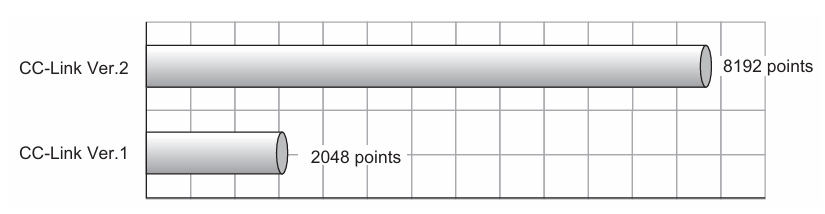
\includegraphics[width=0.7\textwidth]{figures/Chapter01/cclink7.png}
        \caption{So sánh khả năng mở rộng giữa CC-Link Ver.1 và Ver.2}
        \label{fig:cclink_ver2}
    \end{figure}

    % ------------------- 4 -------------------
    \item \textbf{Phòng ngừa sự cố hệ thống}  
    Nhờ cấu trúc nối bus, hệ thống vẫn tiếp tục truyền thông bình thường ngay cả khi một module gặp lỗi. Sau khi module được thay thế hoặc sửa chữa, hệ thống hoạt động trở lại mà không cần cấu hình lại.

\end{enumerate}

%==========================================================================================================
\subsection{Module QJ61BT11N}

Module QJ61BT11N là module Master/Local CC-Link dành cho PLC MELSEC-Q Series \cite{mitsubishi_qj61bt11n_manual}. Hình dạng mặt trước của module được minh họa trong Hình \ref{fig:qj61bt11n}.


\begin{figure}
    \centering
    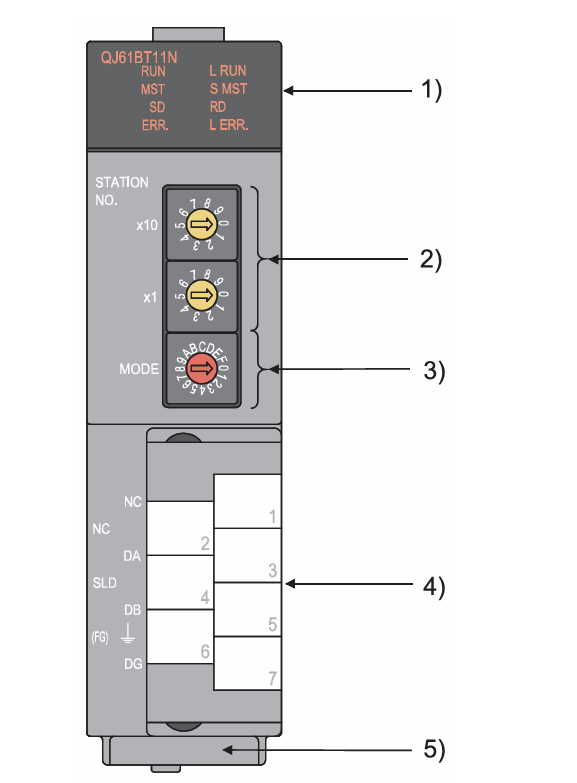
\includegraphics[width=0.5\linewidth]{figures/Chapter01/qj61bt11n.png}
    \caption{Module QJ61BT11N (Master/Local CC-Link)}
    \label{fig:qj61bt11n}
\end{figure}

Các thành phần chính ở mặt trước module gồm:
\begin{itemize}
    \item (1) Đèn LED hiển thị trạng thái,
    \item (2) Thiết lập số thứ tự trạm,
    \item (3) Thiết lập tốc độ truyền thông,
    \item (4) Cổng kết nối cáp CC-Link,
    \item (5) Mã số Serial Number của module.
\end{itemize}

Để cấu hình module CC-Link giao tiếp cần cấu hình địa chỉ của trạm (0 nếu là trạm Master) và Mode (tốc độ truyền nhận). 

% =======================
% PHẦN 3: HỆ CHUYỂN ĐỘNG SERVO
% =======================
\section{Servo motor và Module QD77MS16}

%=======================================================================================
\subsection{Servo và Servo Amplifier}

Servo (bao gồm servo motor và servo amplifier) là hệ truyền động được sử dụng phổ biến trong tự động hóa để điều khiển vị trí, tốc độ và mô-men xoắn với độ chính xác cao. Không giống động cơ thường, servo được trang bị encoder hoặc cảm biến hồi tiếp để thực hiện điều khiển vòng kín (closed-loop control). Nhờ vậy, servo có khả năng đáp ứng nhanh, sai số nhỏ và độ ổn định cao, phù hợp cho các ứng dụng yêu cầu độ chính xác như máy CNC, robot công nghiệp, dây chuyền sản xuất linh kiện điện tử, đóng gói và in ấn.

Một hệ thống servo bao gồm:  
(1) Servo motor,  
(2) Servo amplifier/driver,  
(3) Bộ điều khiển (PLC hoặc motion controller).  
Servo amplifier nhận lệnh từ bộ điều khiển, xử lý phản hồi từ encoder và điều chỉnh dòng điện cấp cho motor để bảo đảm vận hành đúng quỹ đạo đặt trước.

Trong hệ thống này, động cơ sử dụng là \textbf{HG-KR32} kết hợp với \textbf{servo amplifier MR-J4-20B}. Ngoài ra, Mitsubishi Electric cung cấp nhiều dải công suất và chủng loại servo khác nhau phù hợp cho nhiều ứng dụng công nghiệp.

% ---------------- Two images side-by-side ----------------
\begin{figure}[h]
    \centering
    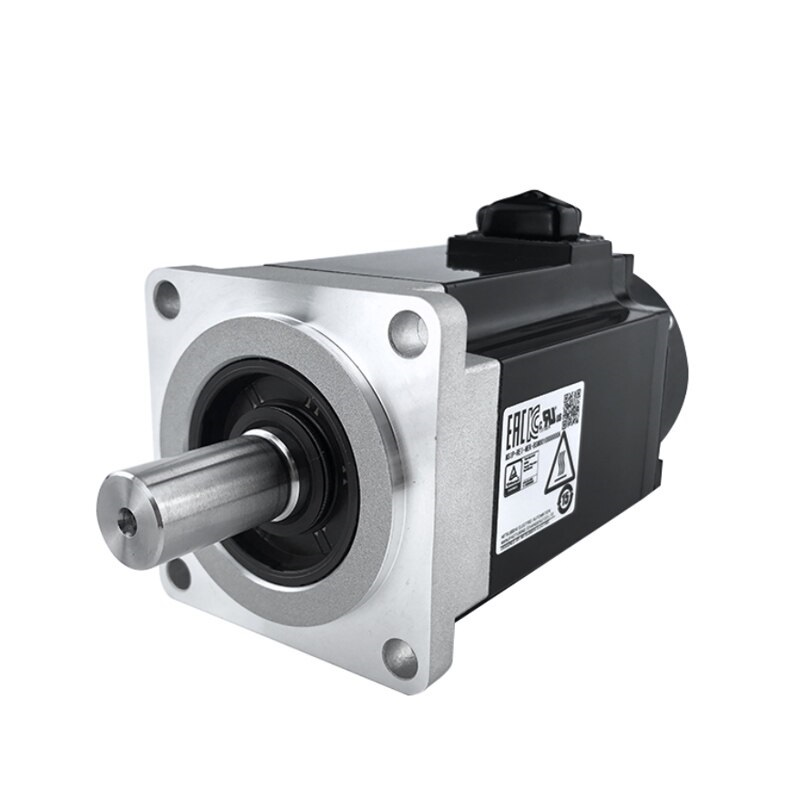
\includegraphics[width=0.48\linewidth]{figures/Chapter01/servo.jpg}
    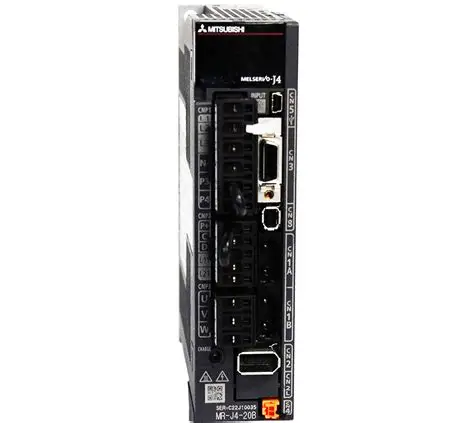
\includegraphics[width=0.48\linewidth]{figures/Chapter01/mrj420b.png}
    \caption{Bộ truyền động servo sử dụng trong hệ thống}
    \label{fig:servo_system}
\end{figure}
% ----------------------------------------------------------

Cấu hình của Driver điều khiển cần đúng với thông số của động cơ Servo.

%===========================================================================================
\subsection{Module QD77MS16}

\textbf{QD77MS16} (Hình \ref{fig:qd77ms}) là module điều khiển chuyển động (Simple Motion Module) thuộc dòng PLC MELSEC-Q của Mitsubishi Electric \cite{mitsubishi_qd77ms_manual}. Module được thiết kế để thực hiện các bài toán điều khiển vị trí, tốc độ và mô-men với độ chính xác cao, hỗ trợ đồng bộ nhiều trục trong hệ thống tự động hóa hiện đại.

\begin{figure}[h]
    \centering
    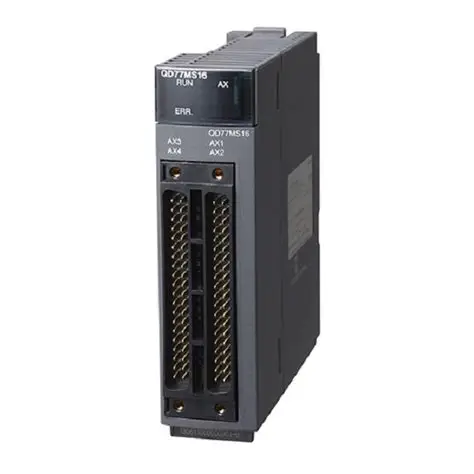
\includegraphics[width=0.42\linewidth]{figures/Chapter01/qd77ms16.png}
    \caption{Module điều khiển chuyển động QD77MS16}
    \label{fig:qd77ms}
\end{figure}

\textbf{Các đặc điểm chính của QD77MS16:}

\begin{itemize}
    \item \textbf{Thời gian khởi động nhanh:}  
    Đạt 0.88 ms (với QD77MS4) trong chế độ điều khiển định vị.

    \item \textbf{Nhiều chức năng điều khiển định vị:}  
    Hỗ trợ điều khiển HPR, điều khiển vị trí, điều khiển tốc độ, chuyển đổi vị trí--tốc độ và điều khiển bằng tay.
    \begin{itemize}
        \item 6 phương pháp HPR khác nhau, hỗ trợ cơ chế HPR retry.  
        \item Điều khiển độc lập từng trục hoặc nội suy 2--4 trục.  
        \item Điều khiển tốc độ--mô-men không qua vòng vị trí.  
        \item Tối đa 600 bộ dữ liệu định vị cho mỗi trục.  
        \item Hỗ trợ thực thi liên tiếp nhiều khối dữ liệu định vị.  
        \item Hai dạng gia tốc/giảm tốc: tuyến tính (trapezoidal) và cong S.  
    \end{itemize}

    \item \textbf{Điều khiển đồng bộ và cam điện tử (E-Cam).}

    \item \textbf{Chức năng phát hiện mark:}  
    Có khả năng latch dữ liệu theo tín hiệu từ DI1--DI4, phù hợp với các ứng dụng cắt theo mark hoặc đồng bộ in ấn.

    \item \textbf{Khả năng bảo trì cao:}  
    Dữ liệu được lưu trong flash ROM, không yêu cầu pin.  
    Thông tin lỗi được lưu và truy xuất trực tiếp từ CPU PLC.

    \item \textbf{Hỗ trợ lệnh chuyên dụng:}  
    Bao gồm Positioning Start, Teaching, và các lệnh tương thích LD77MH/QD75MH giúp tái sử dụng chương trình cũ.

    \item \textbf{Thiết lập và giám sát qua GX Works2:}  
    Dễ dàng cấu hình tham số, kiểm tra wiring, chạy thử, giám sát và debug hệ thống.  
    Có thể kết hợp với \textbf{MR Configurator2} để cấu hình chi tiết servo.

    \item \textbf{Kết nối tốc độ cao qua mạng SSCNET III/H:}  
    Tương thích với MR-J5-B, MR-J4-B, MR-J3-B, MR-JE-B(F), hỗ trợ truyền quang tốc độ cao, giảm nhiễu;  
    cho phép đọc/ghi tham số servo trực tiếp từ module.

    \item \textbf{Hệ thống vị trí tuyệt đối (Absolute Position System):}  
    Sử dụng với MR-J5/J4/J3, chỉ cần gắn pin absolute vào amplifier, không cần proximity dog;  
    khi bật nguồn lại không cần thực hiện HPR.
\end{itemize}


% =======================
% PHẦN 4: ROBOT CÔNG NGHIỆP
% =======================
\section{Robot công nghiệp}

Trong bối cảnh tự động hóa và công nghiệp 4.0 phát triển mạnh, robot công nghiệp, đặc biệt là robot dạng cánh tay, được ứng dụng rộng rãi nhằm tăng năng suất, cải thiện chất lượng và giảm chi phí lao động.

%=====================================================================================
\subsection{Hệ thống Robot Yaskawa}

Một hệ thống robot Yaskawa cơ bản gồm bộ điều khiển (controller), tay máy (manipulator), thiết bị điều khiển cầm tay (programming pendant) và các cáp kết nối.

\begin{itemize}
    \item Cáp programming pendant: kết nối thiết bị cầm tay với bộ điều khiển.
    \item Cáp manipulator: kết nối bộ điều khiển với tay máy, truyền tín hiệu servo và nguồn.
    \item Cáp cấp nguồn: cấp điện (1 pha hoặc 3 pha), yêu cầu có bộ lọc nhiễu.
\end{itemize}

Sơ đồ kết nối tổng quát của hệ thống robot thể hiện trên Hình \ref{fig:yaskawa-dia}.

\begin{figure}[H]
    \centering
    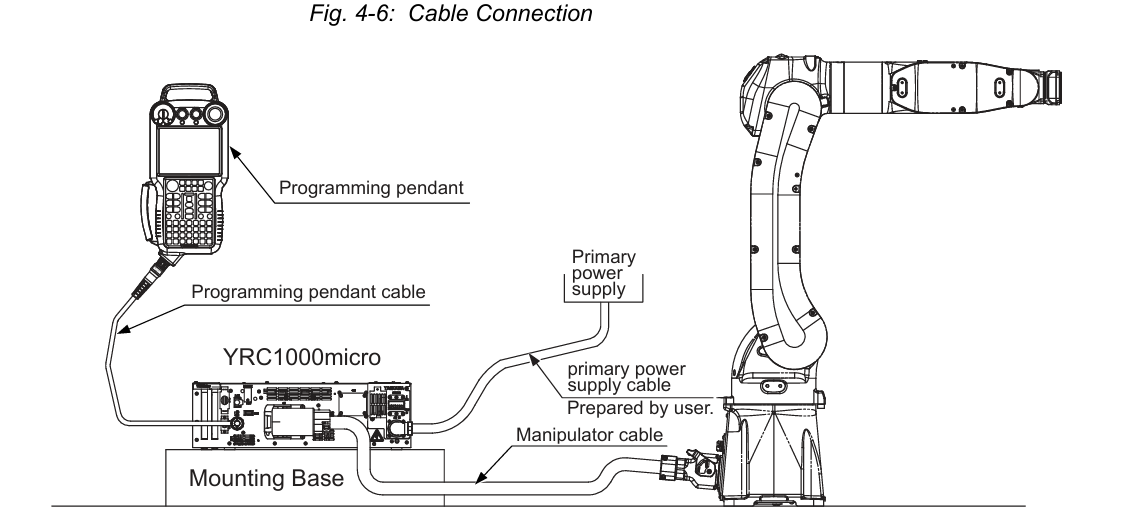
\includegraphics[width=0.75\textwidth]{figures/Chapter2/yaskawa-diagram.png}
    \caption{Sơ đồ tổng quát hệ thống robot công nghiệp}
    \label{fig:yaskawa-dia}
\end{figure}

Hệ thống tại phòng thực hành sử dụng tay máy GP7 và bộ điều khiển YRC1000micro.

% -------------------- GP7 --------------------
\subsubsection{Tay máy GP7}

Robot Yaskawa GP7 (Hình \ref{c2:gp7}) là robot sáu trục với tải trọng 7\,kg, kích thước nhỏ gọn, phù hợp các ứng dụng gắp–đặt, lắp ráp và kiểm tra. GP7 có tốc độ cao, độ chính xác lặp lại khoảng \(\pm 0.01\,\mathrm{mm}\) và dễ lập trình thông qua bộ điều khiển YRC1000micro.

\begin{figure}[H]
    \centering
    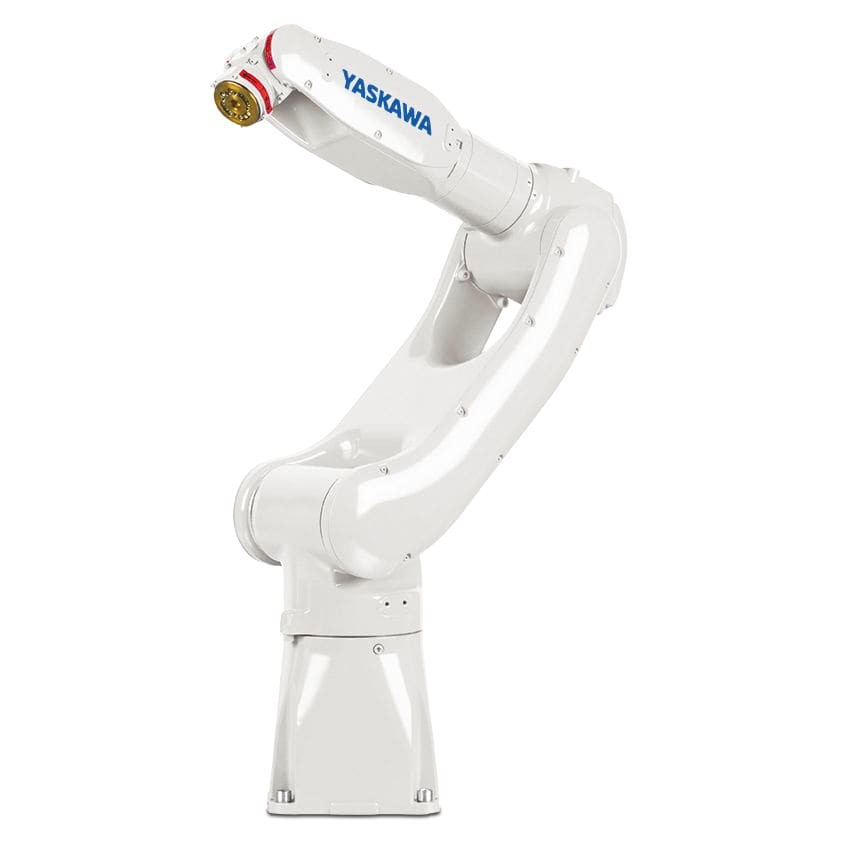
\includegraphics[width=0.5\textwidth]{figures/Chapter2/gp7.jpg}
    \caption{Tay máy GP7}
    \label{c2:gp7}
\end{figure}

Thông số chính:
\begin{itemize}
    \item Tải trọng: 7\,kg
    \item Tầm với ngang: 927\,mm
    \item Tầm với dọc: 1693\,mm
    \item Độ chính xác lặp lại: \(\pm 0.01\,\mathrm{mm}\)
\end{itemize}

Bảng \ref{tab:gp7_axes} trình bày phạm vi chuyển động theo từng trục.

\begin{table}[H]
\centering
\begin{tabularx}{\textwidth}{|c|X|c|c|}
\hline
Trục & Phạm vi (°) & Tốc độ (°/s) & Moment (N·m) \\ \hline
S & \(\pm 170\) & 375 & - \\ \hline
L & \(+145/-65\) & 315 & - \\ \hline
U & \(+190/-70\) & 410 & - \\ \hline
R & \(\pm 190\) & 550 & 17 \\ \hline
B & \(\pm 135\) & 550 & 17 \\ \hline
T & \(\pm 360\) & 1000 & 10 \\ \hline
\end{tabularx}
\caption{Phạm vi chuyển động các trục robot GP7}
\label{tab:gp7_axes}
\end{table}


% -------------------- YRC1000micro --------------------
\subsubsection{Bộ điều khiển YRC1000micro}

\begin{figure}[H]
    \centering
    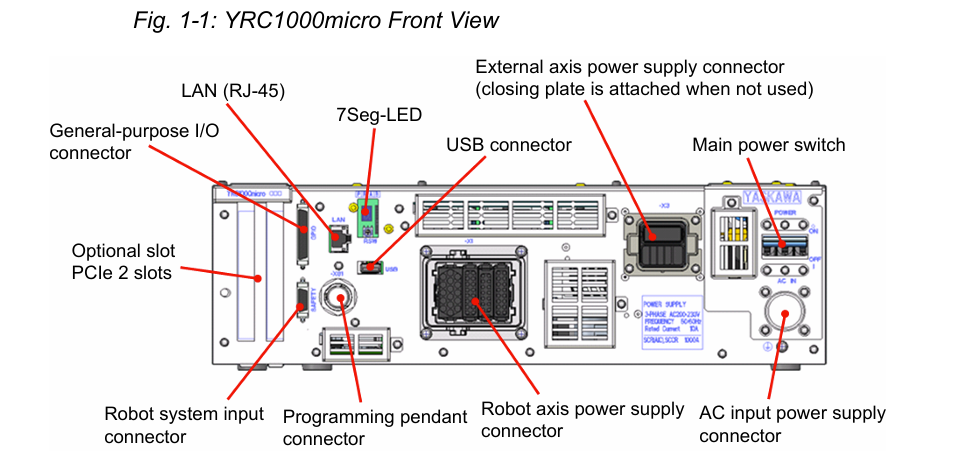
\includegraphics[width=0.75\textwidth]{figures/Chapter2/yrc1000micro.png}
    \caption{Bộ điều khiển YRC1000micro}
    \label{fig:yrc1000}
\end{figure}

Các thành phần chính ở mặt trước controller:

\begin{itemize}
    \item AC input power connector: kết nối nguồn cấp.
    \item Main power switch: bật/tắt nguồn hệ thống.
    \item Robot axis power connector: cấp nguồn và tín hiệu servo cho robot.
    \item USB connector: lưu chương trình/backup dữ liệu.
    \item Programming pendant connector: kết nối pendant.
    \item LAN RJ-45: truyền thông Ethernet/IP.
    \item General-purpose I/O connector: kết nối cảm biến, nút nhấn, relay.
    \item Safety input connector: kết nối tín hiệu an toàn (cửa, dừng khẩn).
\end{itemize}

% -------------------- Pendant --------------------
\subsubsection{Giao diện Teaching Pendant}

Hình \ref{c2:img1} minh họa giao diện chính của pendant.

\begin{figure}[H]
    \centering
    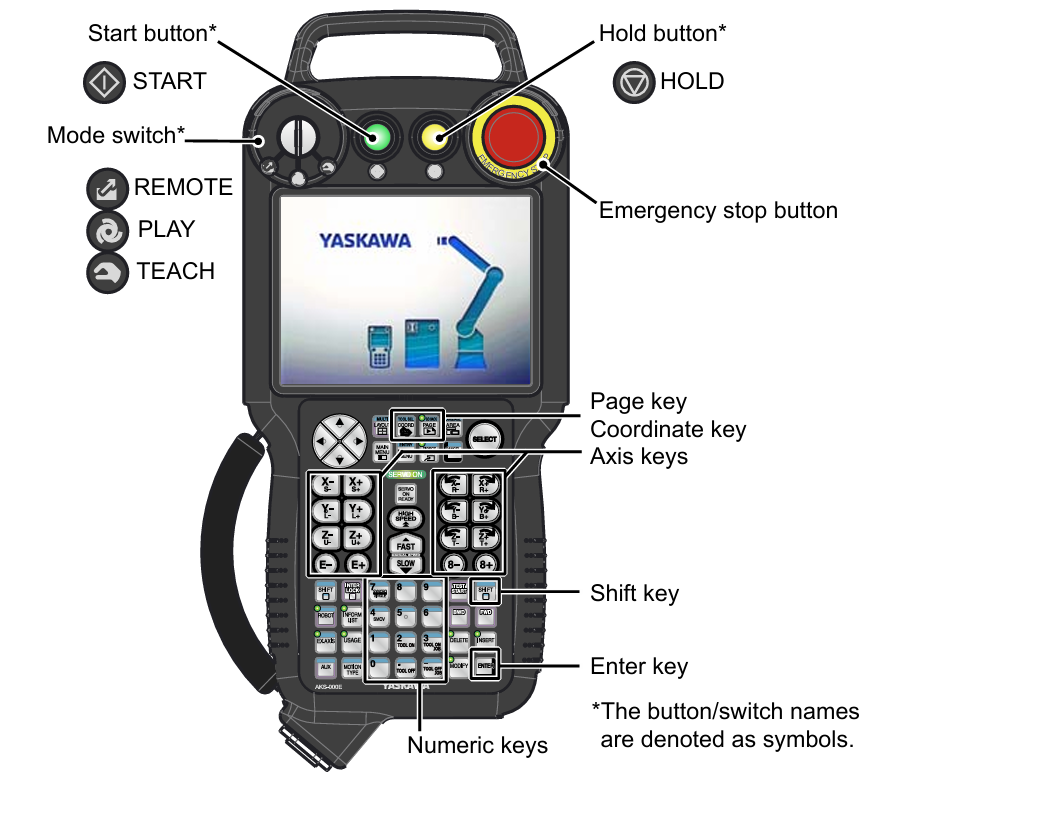
\includegraphics[width=1\textwidth]{figures/Chapter2/image1.png}
    \caption{Giao diện Teach pendant}
    \label{c2:img1}
\end{figure}

\begin{longtable}{|p{0.30\textwidth}|p{0.70\textwidth}|}
\hline
Mục & Mô tả \\ \hline
Phím ký tự / biểu tượng & Các phím như [ENTER]. \\ \hline
Phím trục / phím số & Dùng điều khiển trục hoặc nhập giá trị. \\ \hline
Nhấn đồng thời & Ví dụ [SHIFT]+[COORD]. \\ \hline
Công tắc chế độ & Chọn REMOTE, PLAY hoặc TEACH. \\ \hline
Nút bấm & START, HOLD, EMERGENCY STOP. \\ \hline
Màn hình hiển thị & Các mục menu viết dạng \{JOB\}. \\ \hline
\end{longtable}

% -------------------- Viết chương trình --------------------
Điều kiện trước khi dạy robot: nút \texttt{Emergency Stop} không được nhấn, pendant ở chế độ \texttt{TEACH}, bật nguồn \texttt{SERVO} và giữ công tắc trên tay cầm.

Để tạo chương trình mới:  
\texttt{MAIN MENU} → \texttt{JOB} → \texttt{CREATE NEW JOB} → đặt tên → \texttt{EXECUTE}.

\begin{figure}[H]
    \centering
    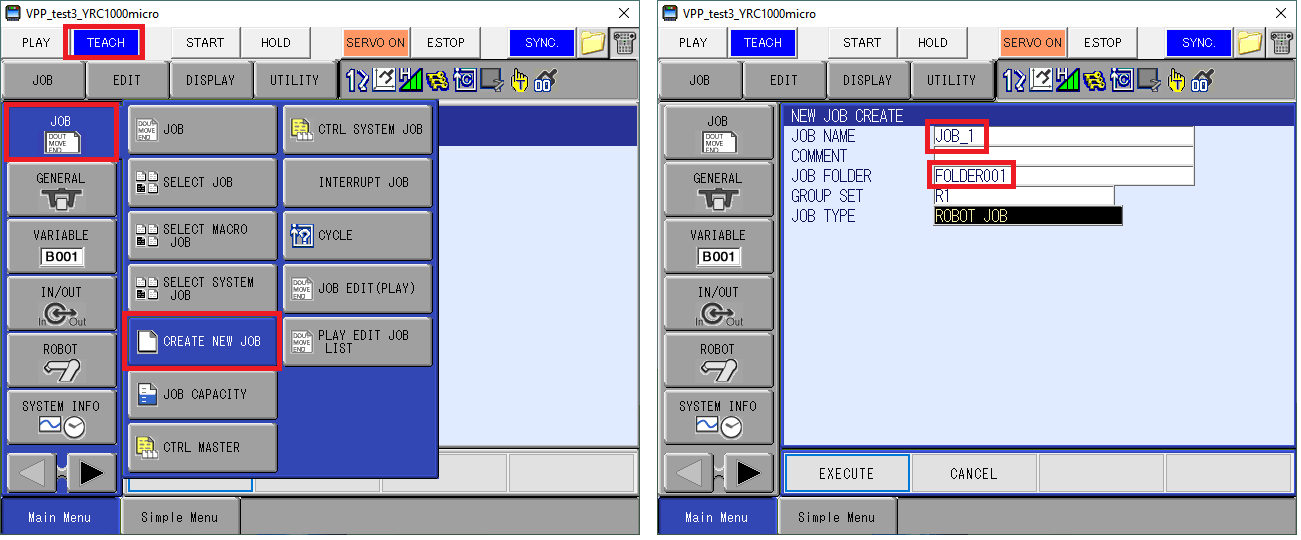
\includegraphics[width=1\textwidth]{figures/Chapter2/yaskawa-process.png}
    \caption{Tạo chương trình mới bằng pendant}
    \label{c2:yakawa-process}
\end{figure}

Màn hình viết chương trình được hiển thị như Hình \ref{c2:job}.

\begin{figure}[H]
    \centering
    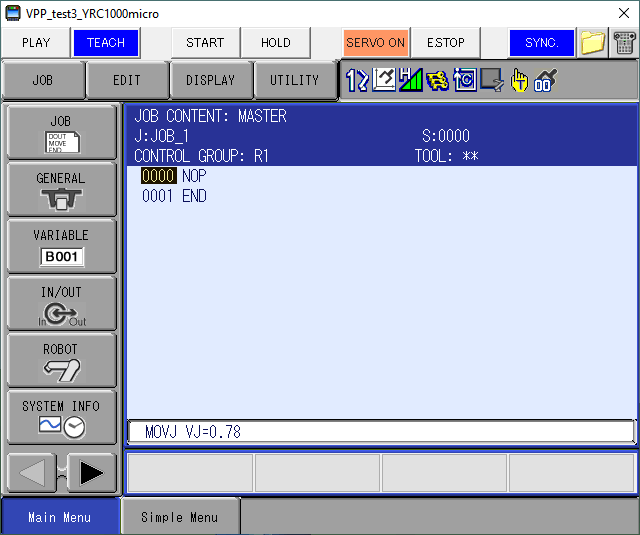
\includegraphics[width=0.75\textwidth]{figures/Chapter2/job.png}
    \caption{Màn hình tạo Job}
    \label{c2:job}
\end{figure}

Cấu trúc một lệnh trong INFORM III gồm:
\begin{center}
\texttt{MOVJ \quad VJ=50.00}
\end{center}

\begin{itemize}
    \item \textbf{Instruction}: loại lệnh cần thực hiện.
    \item \textbf{Additional item}: điều kiện hoặc tham số kèm theo.
\end{itemize}

Các nhóm lệnh trong INFORM III được trình bày trong Bảng \ref{tab:inform-types}.

\begin{table}[H]
\centering
\begin{tabular}{|p{0.30\textwidth}|p{0.68\textwidth}|}
\hline
Loại lệnh & Nội dung \\ \hline
I/O Instruction & Điều khiển tín hiệu I/O \\ \hline
Control Instruction & Điều khiển luồng chương trình \\ \hline
Operating Instruction & Thao tác với biến \\ \hline
Move Instruction & Điều khiển chuyển động của robot \\ \hline
Shift Instruction & Dịch chuyển điểm dạy \\ \hline
Adheres Instruction & Lệnh đi kèm \\ \hline
Work Instruction & Lệnh liên quan thao tác công việc \\ \hline
Optional Instruction & Chức năng tùy chọn \\ \hline
\end{tabular}
\caption{Các nhóm lệnh trong INFORM III}
\label{tab:inform-types}
\end{table}


%===========================================================================================
\subsection{Hệ thống robot Hyundai}

Hệ thống robot Hyundai gồm tay máy và bộ điều khiển, mô tả trong Hình \ref{fig:hyun1}.

\begin{figure}[H]
    \centering
    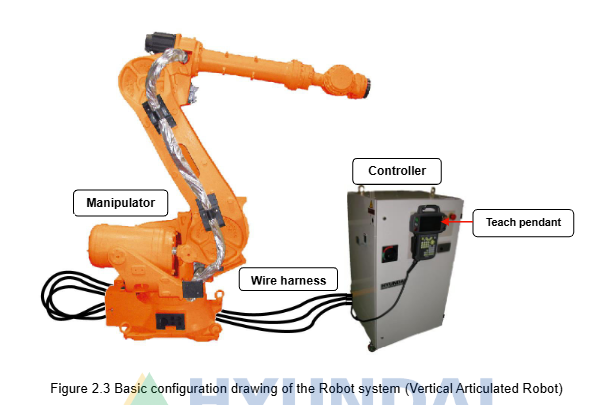
\includegraphics[width=1\textwidth]{figures/Chapter2/hyundai-diagram}
    \caption{Hệ thống robot Hyundai cơ bản}
    \label{fig:hyun1}
\end{figure}

Robot sử dụng là HH7, điều khiển bằng bộ Hi5a.

\begin{figure}[H]
    \centering
    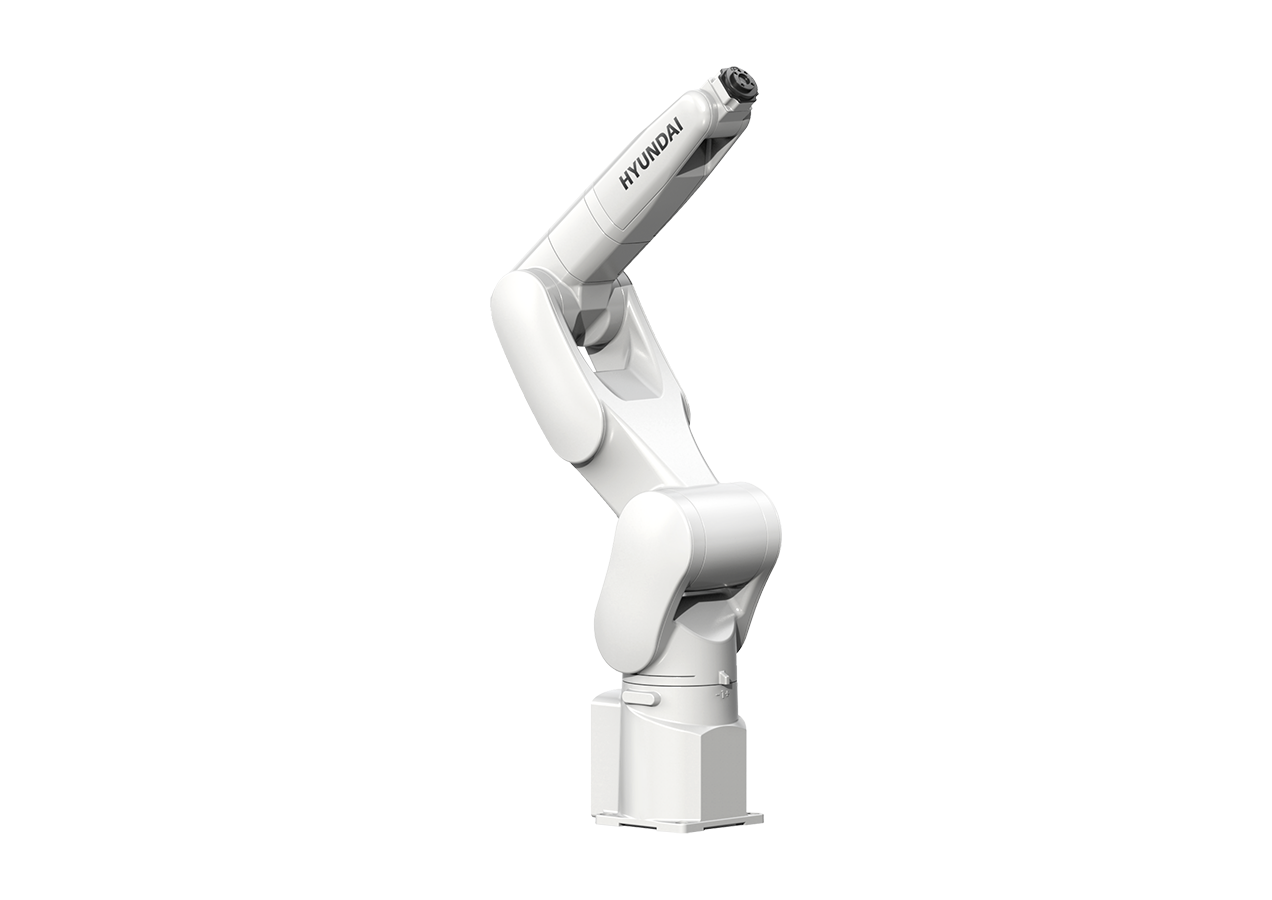
\includegraphics[width=0.6\textwidth]{figures/Chapter2/HH7.png}
    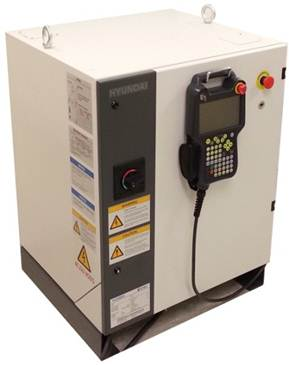
\includegraphics[width=0.3\textwidth]{figures/Chapter2/hi5a.jpg}
    \caption{Tay máy HH7 và Bộ điều khiển Hi5a}
    \label{fig:hyun2}
\end{figure}

Teach pendant của Hi5a có chức năng tương tự pendant của Yaskawa.

\subsubsection{Viết chương trình điều khiển bằng pendant}

Chọn chương trình bằng [SHIFT] + [PROG]. Danh sách chương trình hiển thị như Hình \ref{fig:hyun4}.

\begin{figure}[H]
    \centering
    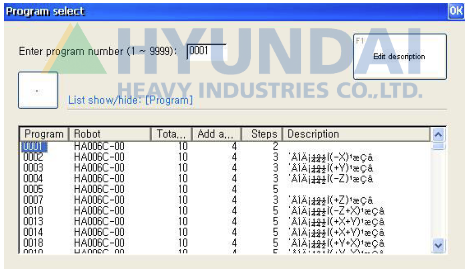
\includegraphics[width=0.75\textwidth]{figures/Chapter2/hyun4.png}
    \caption{Chọn chương trình trên pendant Hi5a}
    \label{fig:hyun4}
\end{figure}

Lệnh robot gồm hai loại:
\begin{itemize}
    \item Lệnh bước: điều khiển chuyển động.
    \item Lệnh chức năng: thực hiện thao tác.
\end{itemize}

\begin{figure}[H]
    \centering
    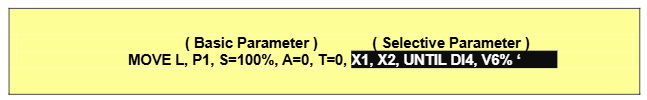
\includegraphics[width=0.75\textwidth]{figures/Chapter2/command.png}
    \caption{Ví dụ một lệnh cơ bản}
    \label{fig:hyun5}
\end{figure}

Mỗi lệnh gồm phần command và các thuộc tính (properties), chia thành:
\begin{itemize}
    \item Thuộc tính bắt buộc.
    \item Thuộc tính tùy chọn.
\end{itemize}

Khi chỉnh sửa, người dùng có thể nhập số, chọn từ menu hoặc nhập ký tự.



% =======================
% PHẦN 4: COMPUTER VISION
% =======================
\section{Thị giác máy tính và mô hình YOLO}
%=======================================================================
\subsection{Thị giác máy tính}
Thị giác máy tính (Computer Vision) là lĩnh vực nghiên cứu cách máy tính hiểu và diễn giải hình ảnh hoặc video, tương tự như cách con người nhận thức thị giác. Trong công nghiệp, thị giác máy đóng vai trò quan trọng trong tự động hóa các tác vụ kiểm tra, giám sát và điều khiển chất lượng.

Một trong những ứng dụng phổ biến nhất của thị giác máy tính là kiểm tra sản phẩm trên dây chuyền sản xuất. Hệ thống camera thu thập hình ảnh sản phẩm, sau đó sử dụng thuật toán xử lý ảnh để phát hiện lỗi như thiếu linh kiện, lắp sai hướng, sai vị trí hoặc khuyết tật bề mặt. So với kiểm tra thủ công, thị giác máy có ưu thế vượt trội về tốc độ, độ chính xác và khả năng hoạt động liên tục.

Ngoài kiểm tra chất lượng, thị giác máy còn được ứng dụng trong các nhiệm vụ như:
\begin{itemize}
    \item \textbf{Nhận dạng ký tự quang học (OCR):} đọc mã bưu chính viết tay trên thư và nhận dạng biển số xe tự động.
    \item \textbf{Kiểm tra máy (Machine inspection):} kiểm tra nhanh các chi tiết để đảm bảo chất lượng bằng stereo vision với hệ thống chiếu sáng chuyên dụng để đo sai số dung sai trên cánh máy bay hoặc thân xe ôtô, hoặc phát hiện lỗi trong khuôn đúc thép bằng ảnh X-ray.
    \item \textbf{Bán lẻ:} nhận dạng vật thể cho các quầy thanh toán tự động và cửa hàng hoàn toàn tự động.
    \item \textbf{Logistics kho:} giao hàng tự động, robot chở pallet và robot gắp hàng bằng tay máy trong kho.
    \item \textbf{Ảnh y tế:} ghép ảnh trước và trong phẫu thuật hoặc nghiên cứu dài hạn về sự thay đổi hình thái não khi con người già đi.
    \item \textbf{Xe tự lái:} di chuyển tự động giữa các thành phố và cả bay tự động.
    \item \textbf{Dựng mô hình 3D (photogrammetry):} xây dựng mô hình 3D hoàn toàn tự động từ ảnh chụp trên không và ảnh drone.
    \item \textbf{Match move:} kết hợp hình ảnh CGI với cảnh quay thực bằng cách theo dõi điểm đặc trưng trong video nguồn để ước tính chuyển động camera 3D và hình dạng môi trường. Kỹ thuật này được sử dụng rộng rãi ở Hollywood, ví dụ như trong phim \textit{Jurassic Park}; ngoài ra còn yêu cầu kỹ thuật tách nền chính xác để chèn đối tượng giữa tiền cảnh và hậu cảnh.
    \item \textbf{Ghi chuyển động (Motion capture – mocap):} sử dụng các marker phản quang từ nhiều camera hoặc kỹ thuật thị giác máy tính khác để thu chuyển động diễn viên cho hoạt hình.
    \item \textbf{Giám sát:} phát hiện người xâm nhập, phân tích giao thông đường cao tốc và giám sát hồ bơi để phát hiện người đuối nước.
\end{itemize}


Trong sản xuất điện tử, thị giác máy đặc biệt quan trọng ở khâu kiểm tra AOI/AVI. Các mô hình học sâu hiện đại như CNN, YOLO giúp hệ thống phân loại và phát hiện linh kiện nhanh, chính xác hơn, giảm đáng kể tỷ lệ lỗi do con người.
%===========================================================================
\subsection{Thư viện OpenCV}

OpenCV (Open Source Computer Vision Library) là thư viện mã nguồn mở được sử dụng rộng rãi trong các hệ thống thị giác máy tính và xử lý ảnh thời gian thực. Thư viện hỗ trợ hàng trăm thuật toán cốt lõi, bao gồm xử lý ảnh cơ bản, phát hiện biên, nhận dạng đối tượng, theo dõi chuyển động, hiệu chỉnh camera và nhiều chức năng nâng cao phục vụ cho tự động hóa công nghiệp. Với ưu điểm tốc độ cao, dễ tích hợp và hoạt động tốt trên nhiều nền tảng (C++, Python, CUDA), OpenCV là lựa chọn phổ biến cho các hệ thống AOI, robot, và các ứng dụng thị giác máy tính hiện đại.

\subsubsection*{Các nhóm chức năng chính của OpenCV}

\begin{itemize}
    \item \textbf{Tiền xử lý ảnh (Image Preprocessing):}  
    Bao gồm chuyển đổi không gian màu (RGB, HSV, LAB), lọc nhiễu (\texttt{GaussianBlur}, \texttt{medianBlur}), cân bằng histogram, trích xuất kênh màu và chuẩn hoá dữ liệu ảnh. Các bước này giúp ổn định chất lượng ảnh đầu vào trước khi gửi vào các thuật toán phát hiện.

    \item \textbf{Biến đổi hình học (Geometric Transformations):}  
    Các phép quay, tịnh tiến, co giãn, cắt (crop), warp affine và warp perspective. Đặc biệt quan trọng trong bài toán căn chỉnh ảnh (image alignment) giữa ảnh chụp thực tế và ảnh mẫu (golden template).

    \item \textbf{Phát hiện biên và đặc trưng (Feature Detection \& Description):}  
    OpenCV hỗ trợ nhiều thuật toán như SIFT, ORB, FAST, BRIEF dùng để trích xuất đặc trưng và mô tả ảnh. Các đặc trưng này được sử dụng trong việc căn chỉnh ảnh, ghép ảnh hoặc theo dõi vật thể.

    \item \textbf{Phân đoạn và trích xuất đối tượng (Segmentation):}  
    Bao gồm thresholding, adaptive thresholding, Otsu, watershed và tìm contour. Đây là bước quan trọng trong việc tách bo mạch PCB khỏi nền hoặc xác định biên dạng linh kiện.

    \item \textbf{Biến đổi tần số và phân tích nâng cao:}  
    Hỗ trợ FFT, DCT, bộ lọc Laplacian, Sobel, Canny. Các thuật toán này phục vụ phát hiện cạnh, phân tích cấu trúc ảnh và tăng độ sắc nét.

    \item \textbf{Đọc/ghi và hiển thị ảnh:}  
    Các hàm như \texttt{imread}, \texttt{imwrite}, \texttt{cvtColor}, \texttt{resize} giúp thao tác ảnh nhanh gọn và thống nhất trong toàn bộ pipeline xử lý.
\end{itemize}

\subsubsection*{Vai trò của OpenCV trong hệ thống}

Trong đề tài này, OpenCV đóng vai trò là nền tảng chính cho toàn bộ pipeline xử lý ảnh từ camera. Các nhiệm vụ chính bao gồm:

\begin{itemize}
    \item Tiền xử lý ảnh để ổn định ánh sáng và màu sắc trước khi phân tích.
    \item Căn chỉnh ảnh (alignment) giữa ảnh thực tế và ảnh mẫu bằng SIFT/ORB.
    \item Tách vùng bo mạch (PCB cropping) dựa trên ngưỡng màu hoặc phân tích kênh màu.
    \item Tính toán độ lệch linh kiện (shift checking) sau khi YOLO phát hiện vị trí.
    \item Giao tiếp với UI và pipeline Python thông qua định dạng ảnh tiêu chuẩn.
\end{itemize}

Nhờ OpenCV, hệ thống đạt được tốc độ xử lý cao, khả năng hoạt động thời gian thực và dễ dàng tích hợp với mô hình học sâu (YOLO) trong quá trình phát hiện lỗi linh kiện.

\subsection{Mạng YOLO - Lược sử phát triển}
\begin{figure}
    \centering
    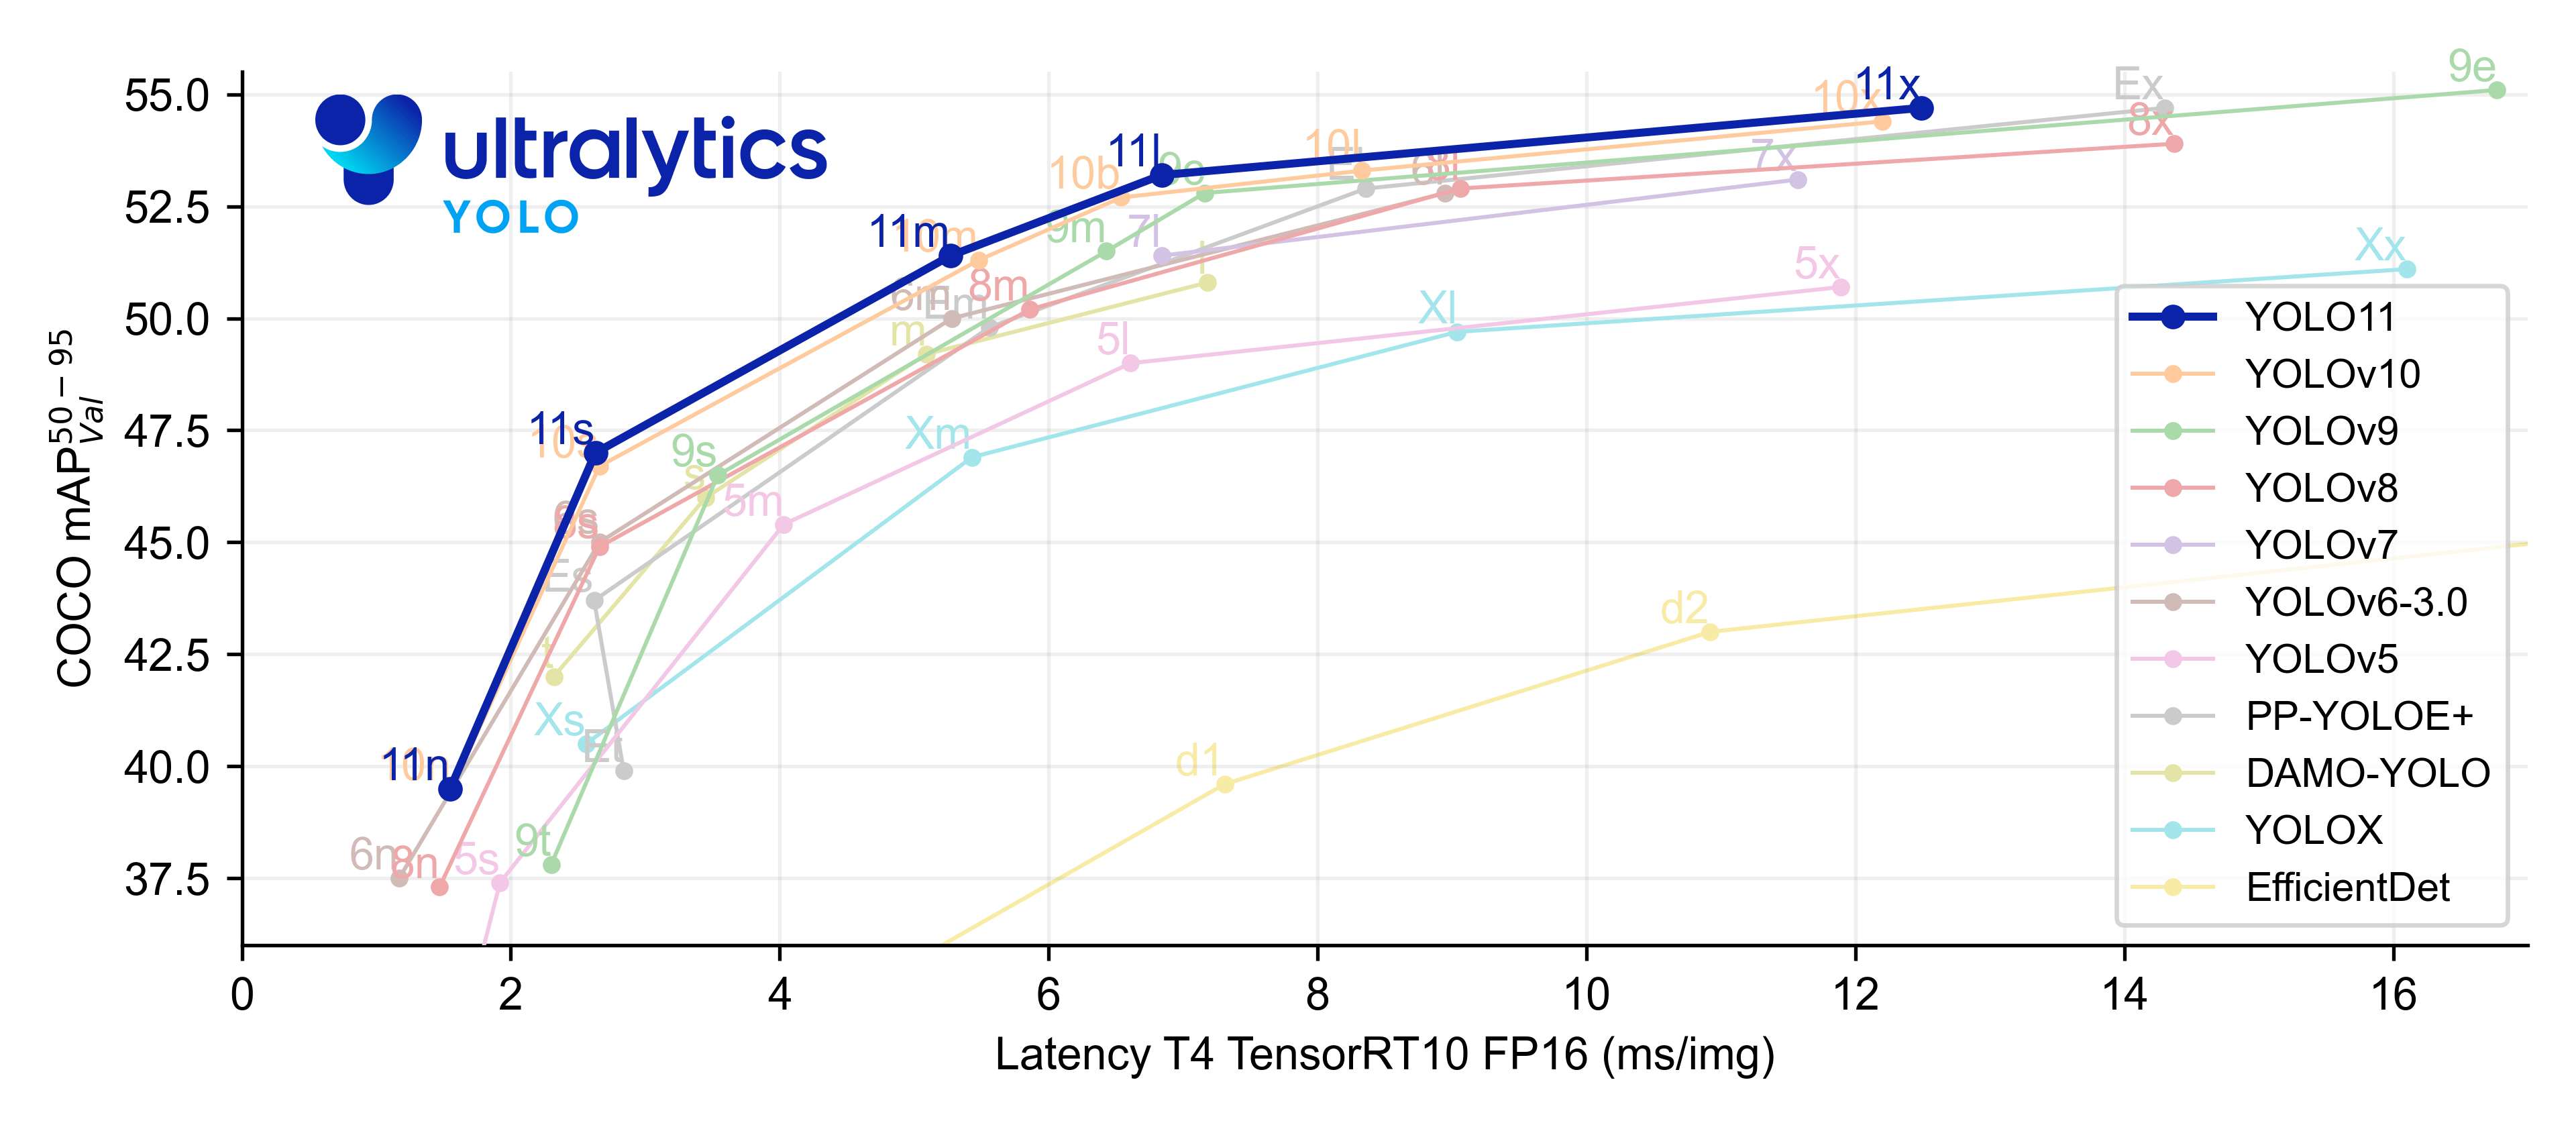
\includegraphics[width=1\textwidth]{figures/Chapter01/performance-comparison.png}
    \caption{YOLO Performance.}
    \label{fig:yolo}
\end{figure}
YOLO (You Only Look Once) là một mô hình nổi tiếng trong lĩnh vực phát hiện đối tượng và phân đoạn ảnh, 
được phát triển bởi Joseph Redmon và Ali Farhadi tại Đại học Washington. 
Ra mắt vào năm 2015, YOLO nhanh chóng được ưa chuộng nhờ tốc độ cao và độ chính xác vượt trội.  

\begin{itemize}
  \item \textbf{YOLOv2 (2016):} Cải tiến so với bản gốc bằng cách bổ sung \textit{batch normalization}, 
  \textit{anchor boxes} và \textit{dimension clusters}.
  
  \item \textbf{YOLOv3 (2018):} Nâng cao hiệu năng với \textit{backbone} hiệu quả hơn, nhiều \textit{anchors} 
  hơn và \textit{spatial pyramid pooling}.
  
  \item \textbf{YOLOv4 (2020):} Giới thiệu các cải tiến như \textit{Mosaic data augmentation}, 
  \textit{anchor-free detection head} và \textit{loss function} mới.
  
  \item \textbf{YOLOv5:} Tiếp tục cải thiện hiệu năng và bổ sung tính năng mới như tối ưu siêu tham số 
  (\textit{hyperparameter optimization}), theo dõi thí nghiệm tích hợp, và tự động xuất ra các định dạng phổ biến.
  
  \item \textbf{YOLOv6 (2022):} Được Meituan phát hành mã nguồn mở, ứng dụng nhiều trong các robot giao hàng tự động.
  
  \item \textbf{YOLOv7:} Mở rộng thêm các tác vụ như ước lượng tư thế (\textit{pose estimation}) trên tập dữ liệu 
  \textit{COCO keypoints}.
  
  \item \textbf{YOLOv8 (2023, Ultralytics):} Bổ sung nhiều tính năng và cải tiến mới, tăng hiệu suất, tính linh hoạt 
  và hiệu quả, đồng thời hỗ trợ đầy đủ các tác vụ thị giác máy tính (\textit{vision AI}).
  
  \item \textbf{YOLOv9:} Giới thiệu phương pháp mới như \textit{Programmable Gradient Information (PGI)} 
  và \textit{Generalized Efficient Layer Aggregation Network (GELAN)}.
  
  \item \textbf{YOLOv10:} Do các nhà nghiên cứu Đại học Thanh Hoa phát triển bằng gói Python của Ultralytics, 
  mang lại tiến bộ trong phát hiện đối tượng thời gian thực nhờ \textit{End-to-End head} loại bỏ nhu cầu sử dụng 
  \textit{Non-Maximum Suppression (NMS)}.
  
  \item \textbf{YOLOv11 (Mới nhất):} Dòng mô hình mới nhất của Ultralytics, đạt hiệu suất tiên tiến 
  (\textit{state-of-the-art}) trên nhiều tác vụ như phát hiện đối tượng, phân đoạn, ước lượng tư thế, 
  theo dõi và phân loại, với khả năng ứng dụng rộng rãi trong nhiều lĩnh vực AI.


\end{itemize}
%====================================================================
\subsection{Ultralytics YOLOv11}
\begin{figure}[h]
    \centering
    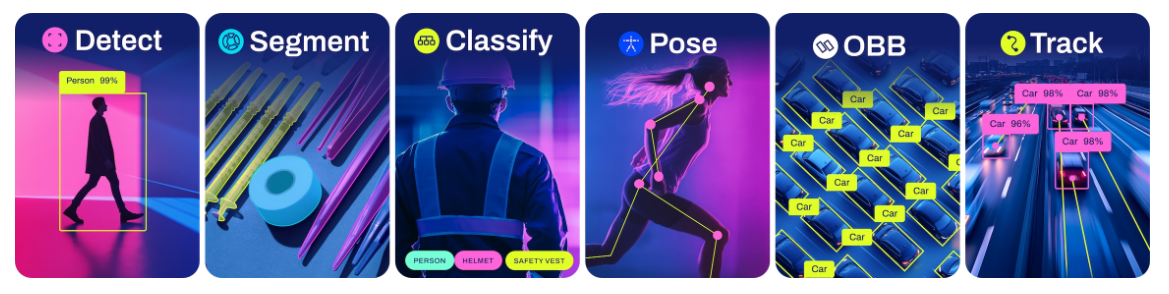
\includegraphics[width=1\textwidth]{figures/Chapter01/yolotasks.png}
    \caption{YOLOv11 Tasks}
    \label{fig:yolov11}
\end{figure}
Ultralytics YOLO11 là một khung AI linh hoạt, hỗ trợ nhiều tác vụ thị giác máy tính khác nhau. Khung này có thể được sử dụng để thực hiện phát hiện đối tượng (detection), phân đoạn ảnh (segmentation), OBB (Oriented Bounding Box), phân loại (classification), và ước lượng tư thế (pose estimation). Mỗi tác vụ có mục tiêu và ứng dụng riêng, cho phép giải quyết nhiều thách thức trong thị giác máy tính chỉ với một framework duy nhất (Hình \ref{fig:yolov11}).

\begin{enumerate}
    \item \textbf{Detection (Phát hiện đối tượng)}: Phát hiện là tác vụ chính được hỗ trợ bởi YOLO11. Nó bao gồm việc xác định các đối tượng trong ảnh hoặc video và vẽ hộp bao quanh (bounding box) chúng. Các đối tượng được phân loại dựa trên đặc trưng. YOLO11 có thể phát hiện nhiều đối tượng trong một ảnh với độ chính xác và tốc độ cao, phù hợp cho các ứng dụng thời gian thực như giám sát an ninh và xe tự hành.
    \item \textbf{Segmentation (Phân đoạn ảnh)}: Phân đoạn chia ảnh thành nhiều vùng dựa trên nội dung, với độ chính xác đến từng pixel. Ứng dụng điển hình gồm chẩn đoán y tế, phân tích nông nghiệp, và kiểm soát chất lượng. YOLO11 triển khai một biến thể của kiến trúc U-Net để đạt hiệu quả cao.
    \item \textbf{Classification (Phân loại ảnh)}: Phân loại gán nhãn cho toàn bộ ảnh dựa trên nội dung. YOLO11 sử dụng biến thể của EfficientNet để đạt hiệu năng cao. Tác vụ này quan trọng trong thương mại điện tử, kiểm duyệt nội dung, và theo dõi động vật hoang dã.
    \item \textbf{Pose Estimation (Ước lượng tư thế)}: Ước lượng tư thế phát hiện các điểm mốc (keypoints) trong ảnh hoặc video để theo dõi chuyển động hoặc ước lượng dáng điệu. Các điểm mốc có thể là khớp cơ thể, đặc điểm khuôn mặt, hoặc các điểm quan trọng khác. YOLO11 cho độ chính xác cao, ứng dụng trong thể dục, phân tích thể thao, và tương tác người–máy.
    \item \textbf{OBB (Oriented Bounding Box – Hộp bao định hướng)}: OBB mở rộng phát hiện đối tượng bằng cách thêm thông tin góc xoay, giúp định vị chính xác các vật thể bị nghiêng hoặc xoay. Điều này đặc biệt hữu ích trong phân tích ảnh hàng không, xử lý tài liệu, và các ứng dụng công nghiệp. YOLO11 hỗ trợ OBB với tốc độ và độ chính xác cao.
\end{enumerate}

%%%%%%%%%%%%%%%%%%%%%%%%%%%%%%%%%%%%%%%%%%%%%%%%%%%%%%%%%%%%%%%
\section{Tổng quan về giao thức OPC UA}

OPC UA (OPC Unified Architecture, IEC 62541) là tiêu chuẩn truyền thông mở được sử dụng rộng rãi trong lĩnh vực tự động hoá công nghiệp. Giao thức cung cấp khả năng trao đổi dữ liệu an toàn, độc lập nền tảng và đáng tin cậy giữa các thiết bị, PLC, robot và các hệ thống phần mềm. OPC UA hỗ trợ cả hai mô hình giao tiếp: client–server và publish/subscribe (PubSub), cho phép triển khai linh hoạt trong nhiều kiến trúc mạng công nghiệp và mạng doanh nghiệp.

OPC UA được phát triển nhằm khắc phục các hạn chế của OPC DA vốn phụ thuộc vào Windows DCOM, không tương thích tốt với tường lửa và thiếu tính mở. Phiên bản đầu tiên của OPC UA được công bố vào năm 2006; phiên bản 1.04 (2017) bổ sung cơ chế PubSub và các chính sách bảo mật nâng cao. Trong đặc tả OPC UA, xác thực, ký số và mã hoá dữ liệu được nhấn mạnh mạnh mẽ trong cả hai mô hình truyền thông.

Với mô hình thông tin tích hợp theo IEC 62541, OPC UA cho phép mô tả dữ liệu, thuộc tính và chức năng của thiết bị theo cấu trúc phân cấp thống nhất. Nhờ đó, OPC UA không chỉ truyền dữ liệu quá trình (set-point, measured value, tham số vận hành) mà còn định nghĩa ý nghĩa của dữ liệu, giúp thiết lập các quy trình giao tiếp hiệu quả giữa PLC và các tầng phần mềm cấp cao như MES hoặc ERP. Các thiết bị trong hệ thống công nghiệp có thể vừa đóng vai trò OPC UA Server vừa là OPC UA Client, hỗ trợ trao đổi dữ liệu ngang và dọc trong dây chuyền.

Trong bối cảnh Industry 4.0 và IIoT, OPC UA được xem là chuẩn truyền thông cốt lõi. Mô hình kiến trúc tham chiếu RAMI 4.0 (2015) khuyến nghị sử dụng OPC UA cho lớp truyền thông, khiến OPC UA trở thành yêu cầu bắt buộc đối với các thiết bị “Industry 4.0-ready”. Ngoài TCP và HTTPS trong mô hình client–server, OPC UA PubSub còn có thể sử dụng UDP, AMQP hoặc MQTT, phù hợp cho các ứng dụng tốc độ cao và mạng phân tán.

\begin{figure}[h]
    \centering
    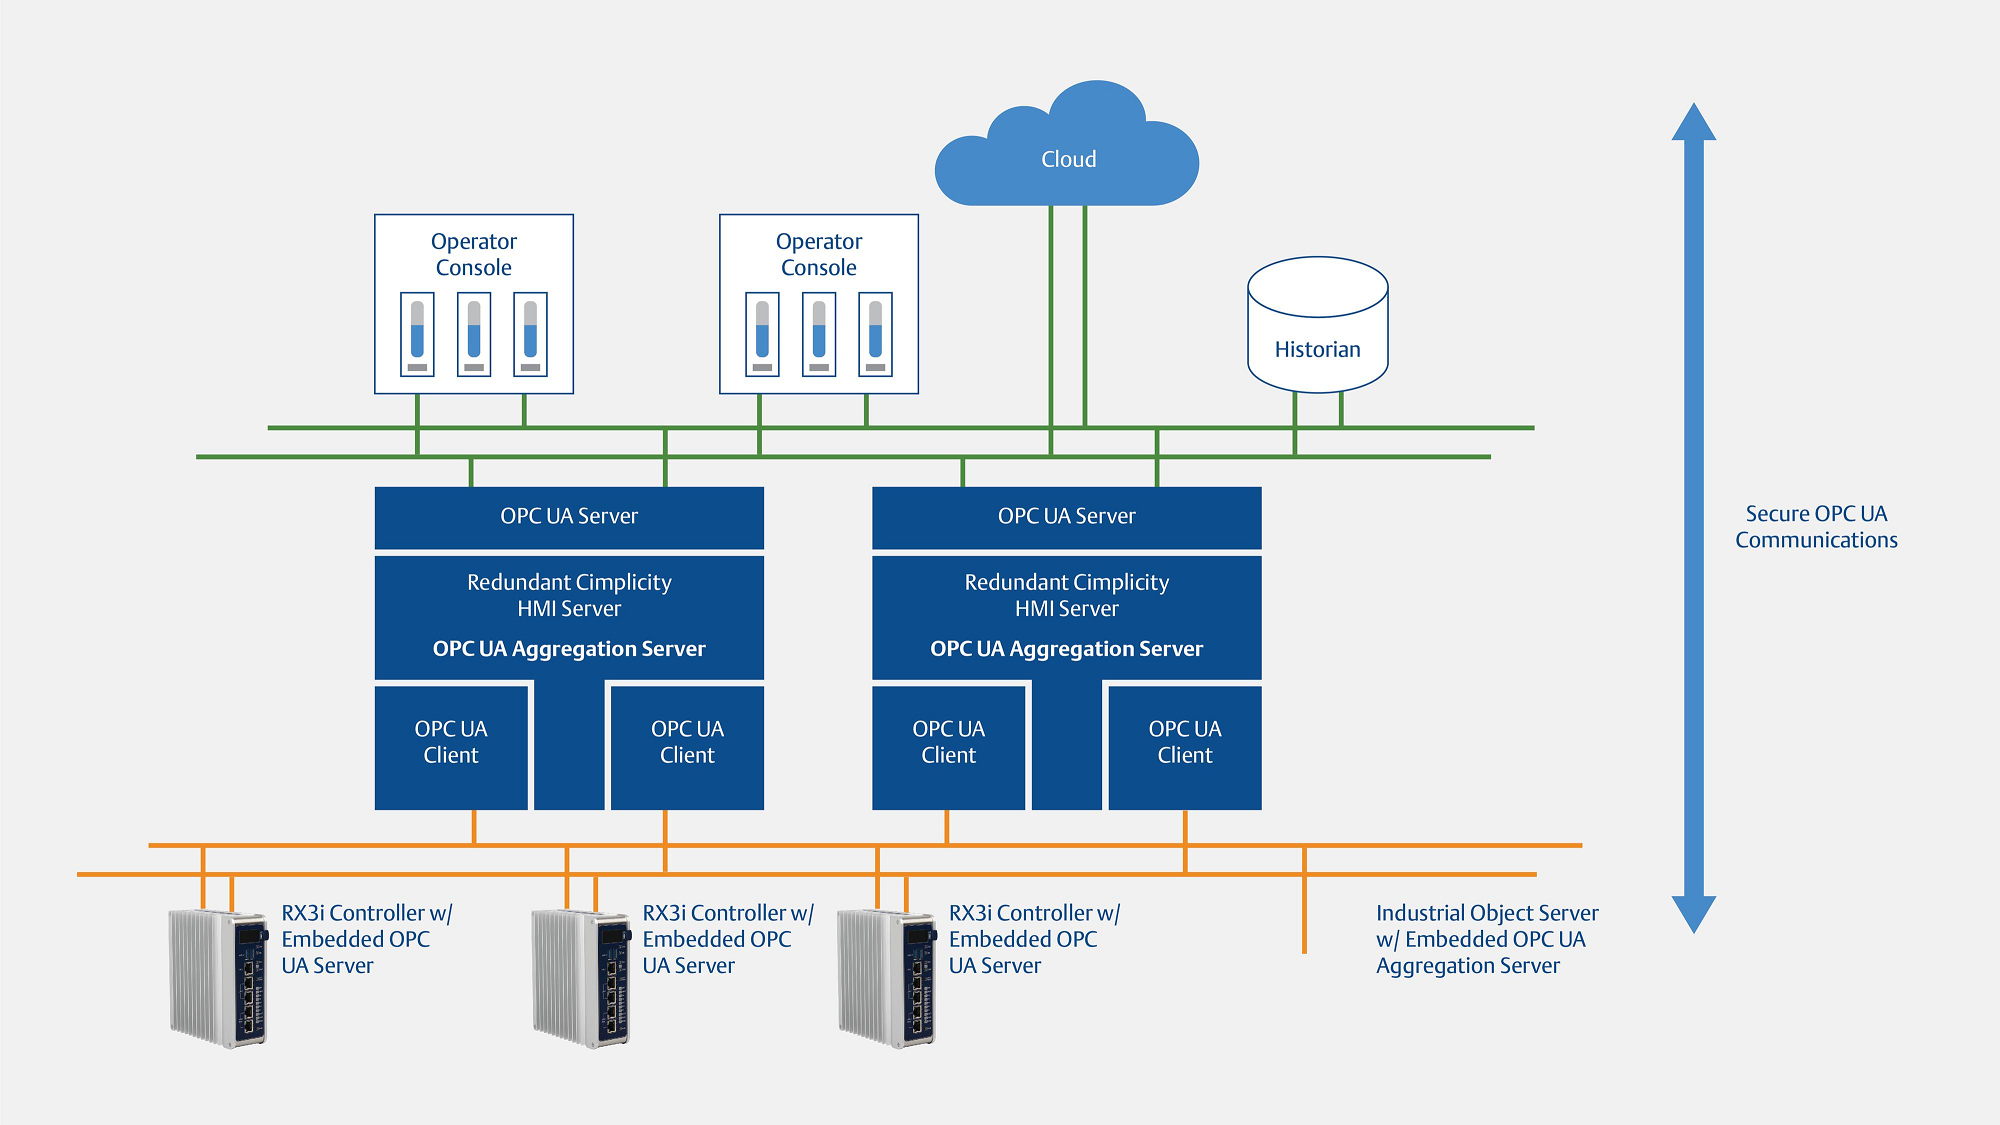
\includegraphics[width=1\textwidth]{figures/Chapter2/opcua.png}
    \caption{Tổng quan OPC UA}
    \label{c2:opcua}
\end{figure}
OPC UA ngày nay không chỉ được triển khai trong PLC, robot và cảm biến mà còn xuất hiện trên các thiết bị nhúng, chip, và thiết bị IoT. Khả năng kết nối chuẩn hóa tạo điều kiện truyền dữ liệu lên các nền tảng đám mây; các tính năng bổ trợ như Cloud Relay giúp vượt qua giới hạn tường lửa. Cùng với sự phát triển của 5G, WiFi 6/7 và các kỹ thuật mạng hỗ trợ QoS, OPC UA hướng tới truyền thông mang tính quyết định (deterministic) cho các ứng dụng công nghiệp thời gian thực.





\chapter{Xây dựng hệ thống }
% =======================
% PHẦN 1: SƠ ĐỒ KHỐI
% =======================
% =======================

\section{Sơ đồ khối hệ thống}

Hệ thống tổng quát chia ra hai thành phần chính: PC Side và PLC Side.  
Hai bên giao tiếp với nhau thông qua giao thức OPC UA.

\begin{figure}[h]
    \centering
    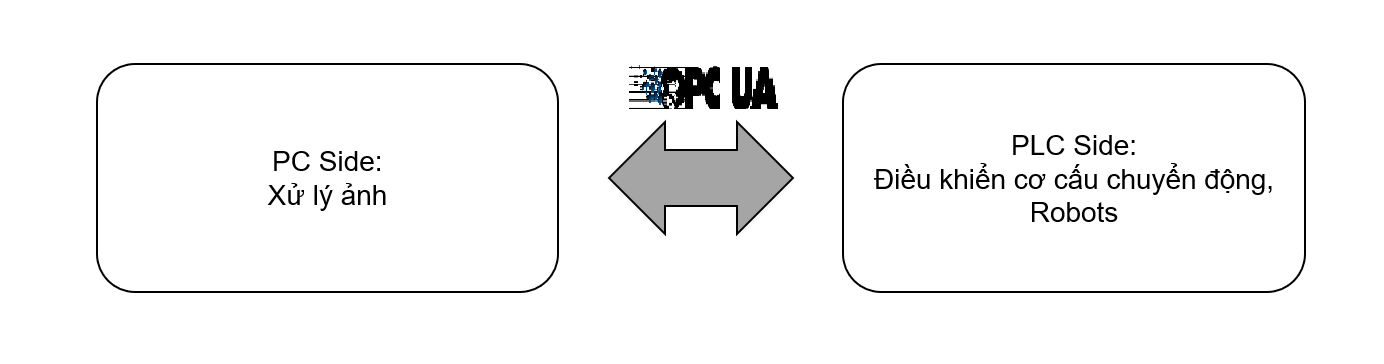
\includegraphics[width=1\textwidth]{figures/Chapter3/image1.png}
    \caption{Cấu trúc tổng quát hệ thống}
\end{figure}

\begin{enumerate}
    \item \textbf{PC Side:} 
    Máy tính đóng vai trò xử lý thị giác máy tính, chạy thuật toán phát hiện lỗi, phân loại NG/OK và trả kết quả về PLC thông qua OPC UA. Hệ thống bao gồm camera công nghiệp, phần mềm xử lý ảnh và module giao tiếp OPC UA Client. Cấu trúc hệ thống như Hình~\ref{c3:pcside}. 

    \begin{figure}[h]
        \centering
        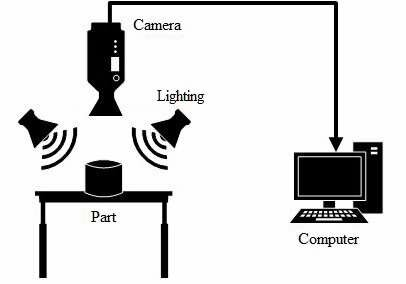
\includegraphics[width=0.5\textwidth]{figures/Chapter3/pcside.png}
        \caption{PC Side}
        \label{c3:pcside}
    \end{figure}

    \item \textbf{PLC Side:}  
    Hệ thống PLC bao gồm nguồn, CPU, module giao tiếp CC-Link (QJ61BT11N), module điều khiển chuyển động QD77MS16, màn hình HMI, các remote I/O, các trạm Robot, hệ thống servo và bộ khuếch đại.  
    Sơ đồ khối PLC Side được thể hiện trong Hình~\ref{c3:plcside}.

    \begin{figure}[h]
        \centering
        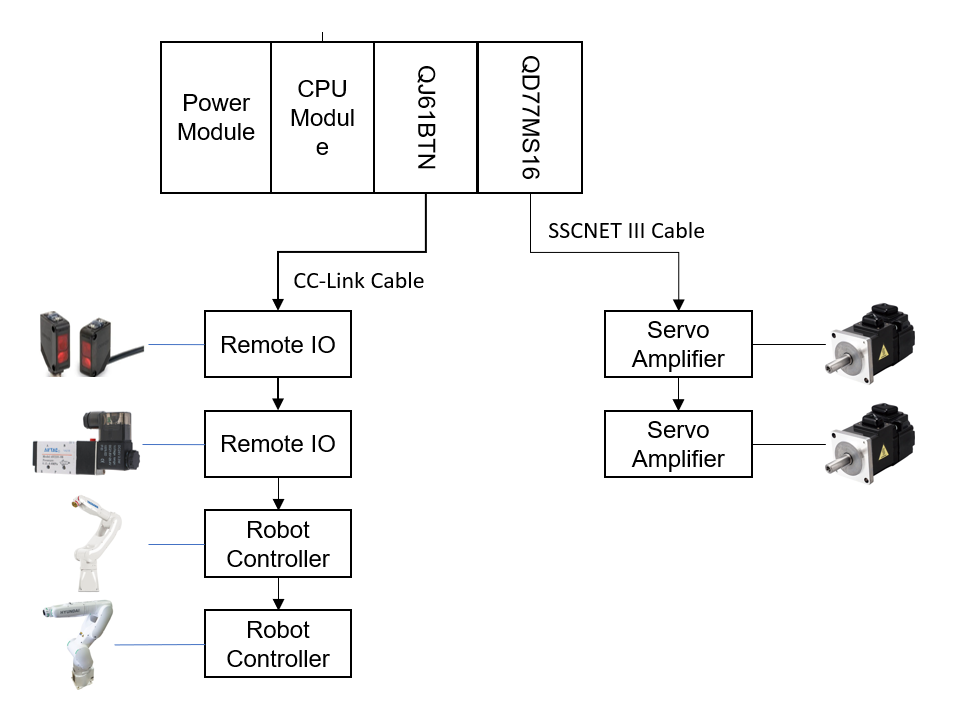
\includegraphics[width=1\textwidth]{figures/Chapter3/image2.png}
        \caption{PLC Side}
        \label{c3:plcside}
    \end{figure}

    \item \textbf{OPC UA:}  
    OPC UA (OPC Unified Architecture) được dùng để giao tiếp giữa PLC Side và PLC Side. 
\end{enumerate}


% =======================
% PHẦN 2: THUẬT TOÁN ĐIỀU KHIỂN
% =======================



\section{Thuật toán điều khiển}

Hệ thống tự động dựa trên luồng di chuyển của sản phẩm được chia thành năm quá trình chính như Hình~\ref{c3:workflow}:

\begin{figure}
    \centering
    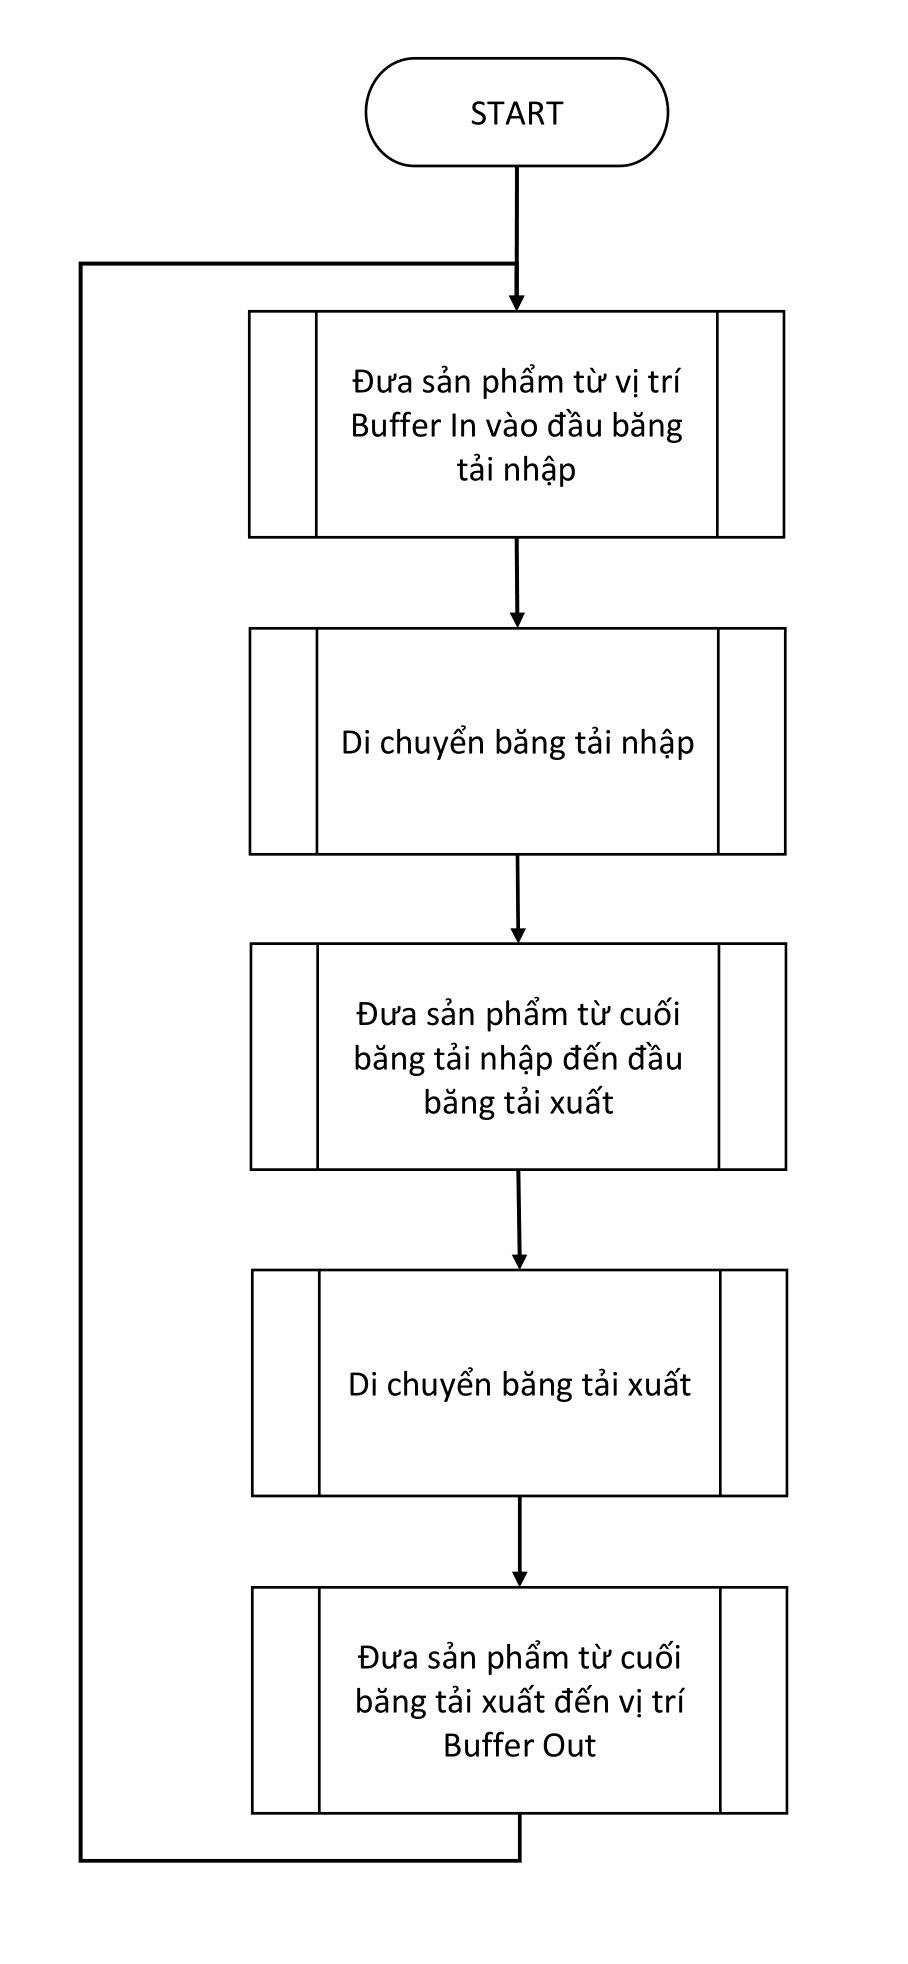
\includegraphics[width=0.68\textwidth]{figures/Chapter3/workflow.png}
    \caption{Quy trình tổng quát}
    \label{c3:workflow}
\end{figure}

\begin{enumerate}
    \item Đưa sản phẩm từ vị trí Buffer In vào đầu băng tải nhập bằng robot Hyundai.
    \item Di chuyển băng tải nhập đưa sản phẩm từ đầu băng tải đến vị trí chụp ảnh; sau khi chụp ảnh, băng tải tiếp tục di chuyển sản phẩm đến cuối băng tải.
    \item Đưa sản phẩm từ cuối băng tải nhập đến đầu băng tải xuất bằng robot Yaskawa.
    \item Di chuyển băng tải xuất từ đầu băng tải đến cuối băng tải.
    \item Đưa sản phẩm từ cuối băng tải xuất đến vị trí Buffer Out bằng robot Hyundai.
\end{enumerate}

Việc phân tách hệ thống thành các quá trình riêng biệt giúp dễ dàng xây dựng lưu trình điều khiển chi tiết, đồng thời đơn giản hóa quá trình lập trình và kiểm soát hoạt động của toàn hệ thống.
%=================================
\newpage
\subsection{Quá trình 1: Đưa sản phẩm từ Buffer In vào đầu băng tải nhập}

\begin{figure}[h]
    \centering
    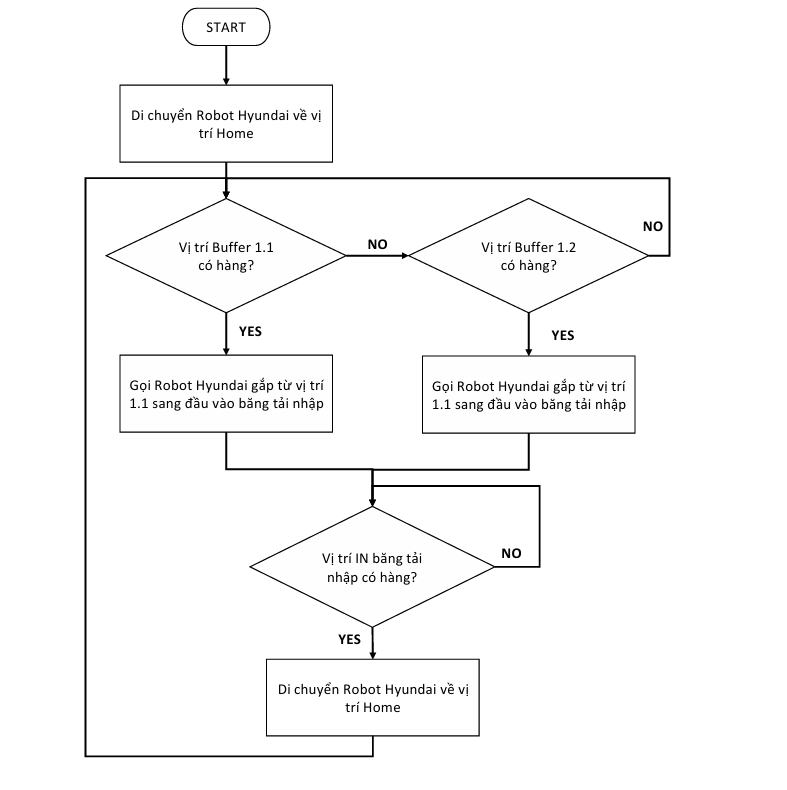
\includegraphics[width=1\textwidth]{figures/Chapter3/workflow1.png}
    \caption{Quá trình 1.}
    \label{c3:workflow1}
\end{figure}
%=================================================
\newpage
\subsection{Quá trình 2: Di chuyển băng tải nhập}

\begin{figure}[h]
    \centering
    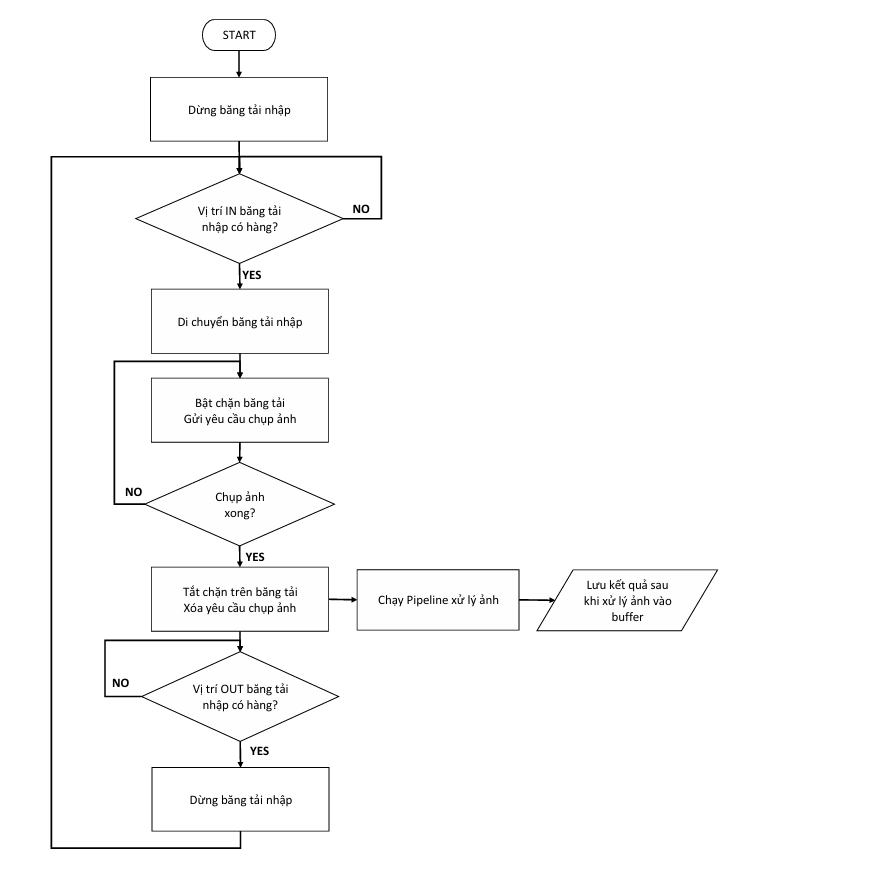
\includegraphics[width=1\textwidth]{figures/Chapter3/workflow2.png}
    \caption{Quá trình 2.}
    \label{c3:workflow2}
\end{figure}
%=================================================
\newpage
\subsection{Quá trình 3: Đưa sản phẩm từ băng tải nhập vào băng tải xuất}

\begin{figure}[h]
    \centering
    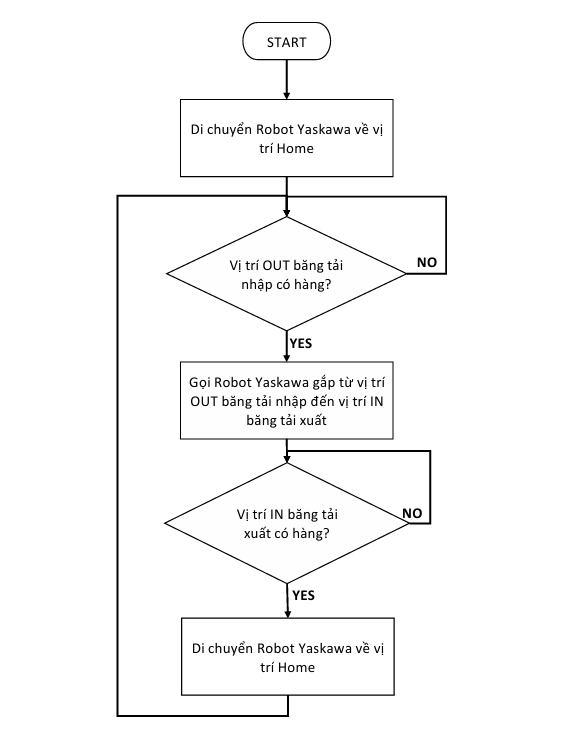
\includegraphics[width=0.8\textwidth]{figures/Chapter3/workflow3.png}
    \caption{Quá trình 3.}
    \label{c3:workflow3}
\end{figure}
%=================================================
\newpage
\subsection{Quá trình 4: Di chuyển băng tải xuất}

\begin{figure}[h]
    \centering
    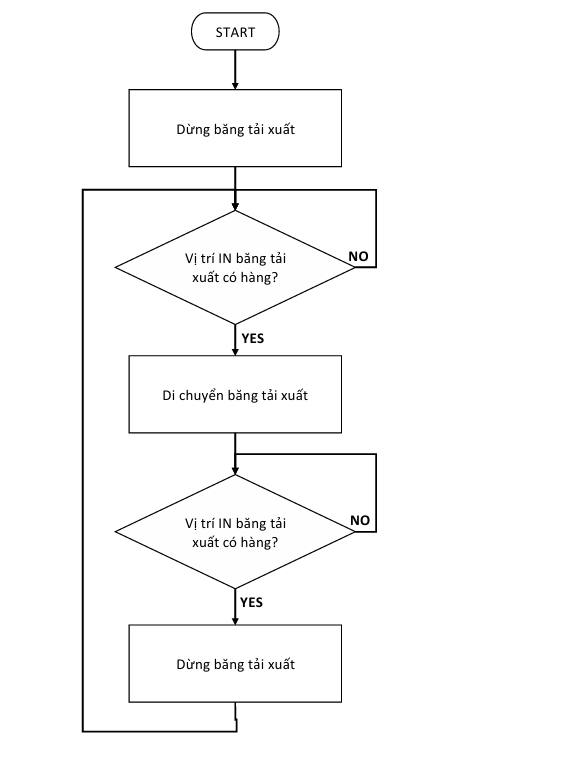
\includegraphics[width=0.8\textwidth]{figures/Chapter3/workflow4.png}
    \caption{Quá trình 4.}
    \label{c3:workflow4}
\end{figure}
%======================================================
\newpage
\subsection{Quá trình 5: Đưa sản phẩm từ băng tải xuất đến Buffer Out}

\begin{figure}[h]
    \centering
    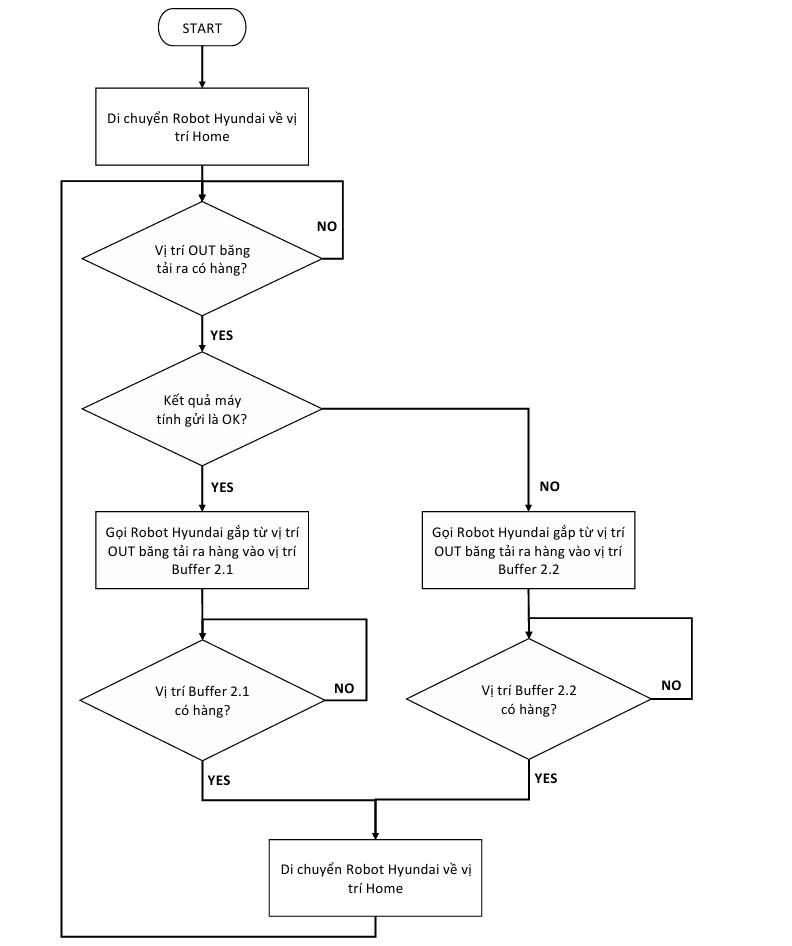
\includegraphics[width=0.8\textwidth]{figures/Chapter3/workflow5.png}
    \caption{Quá trình 5.}
    \label{c3:workflow5}
\end{figure}


% =======================
% PHẦN 3: CẤU HÌNH HỆ THỐNG
% =======================
\newpage



\section{Cấu hình hệ thống}
%====================================================================================

\subsection{Cấu hình hệ thống PLC và module}
Công cụ lập trình dùng cho PLC Mitsubishi Q Series là phần mềm GX Works2.
Khi khởi tạo project cần chọn dòng PLC (Q mode); loại CPU (Q13UDV); loại project (Simple Project) và ngôn ngữ lập trình sử dụng trong project (Ladder). Cấu hình như Hình \ref{c3:newprj}.

Sau khi đã tạo thành công project mới, cần cấu hình hệ thống PLC tương ứng với phần cứng sử dụng. 
\begin{figure} [h]
    \centering
    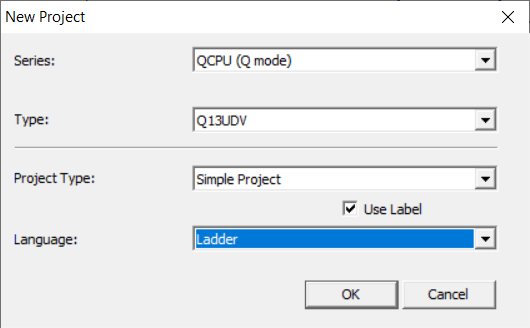
\includegraphics[width=0.75\linewidth]{figures/Chapter3/newprj.png}
    \caption{Cấu hình New Project}
    \label{c3:newprj}
\end{figure}
%\newpage
\begin{enumerate}
    \item Cấu hình base unit và các module giống với thiết lập phần cứng như Hình \ref{c3:hardware}. 
    Thiết lập thông tin của base unit và vị trí module trong GX Works2 như Hình \ref{c3:io} tại \textit{Parameter} $\rightarrow$ \textit{PLC Parameter} $\rightarrow$ \textit{I/O Assignment}.
    \begin{figure}[H]
    \centering
    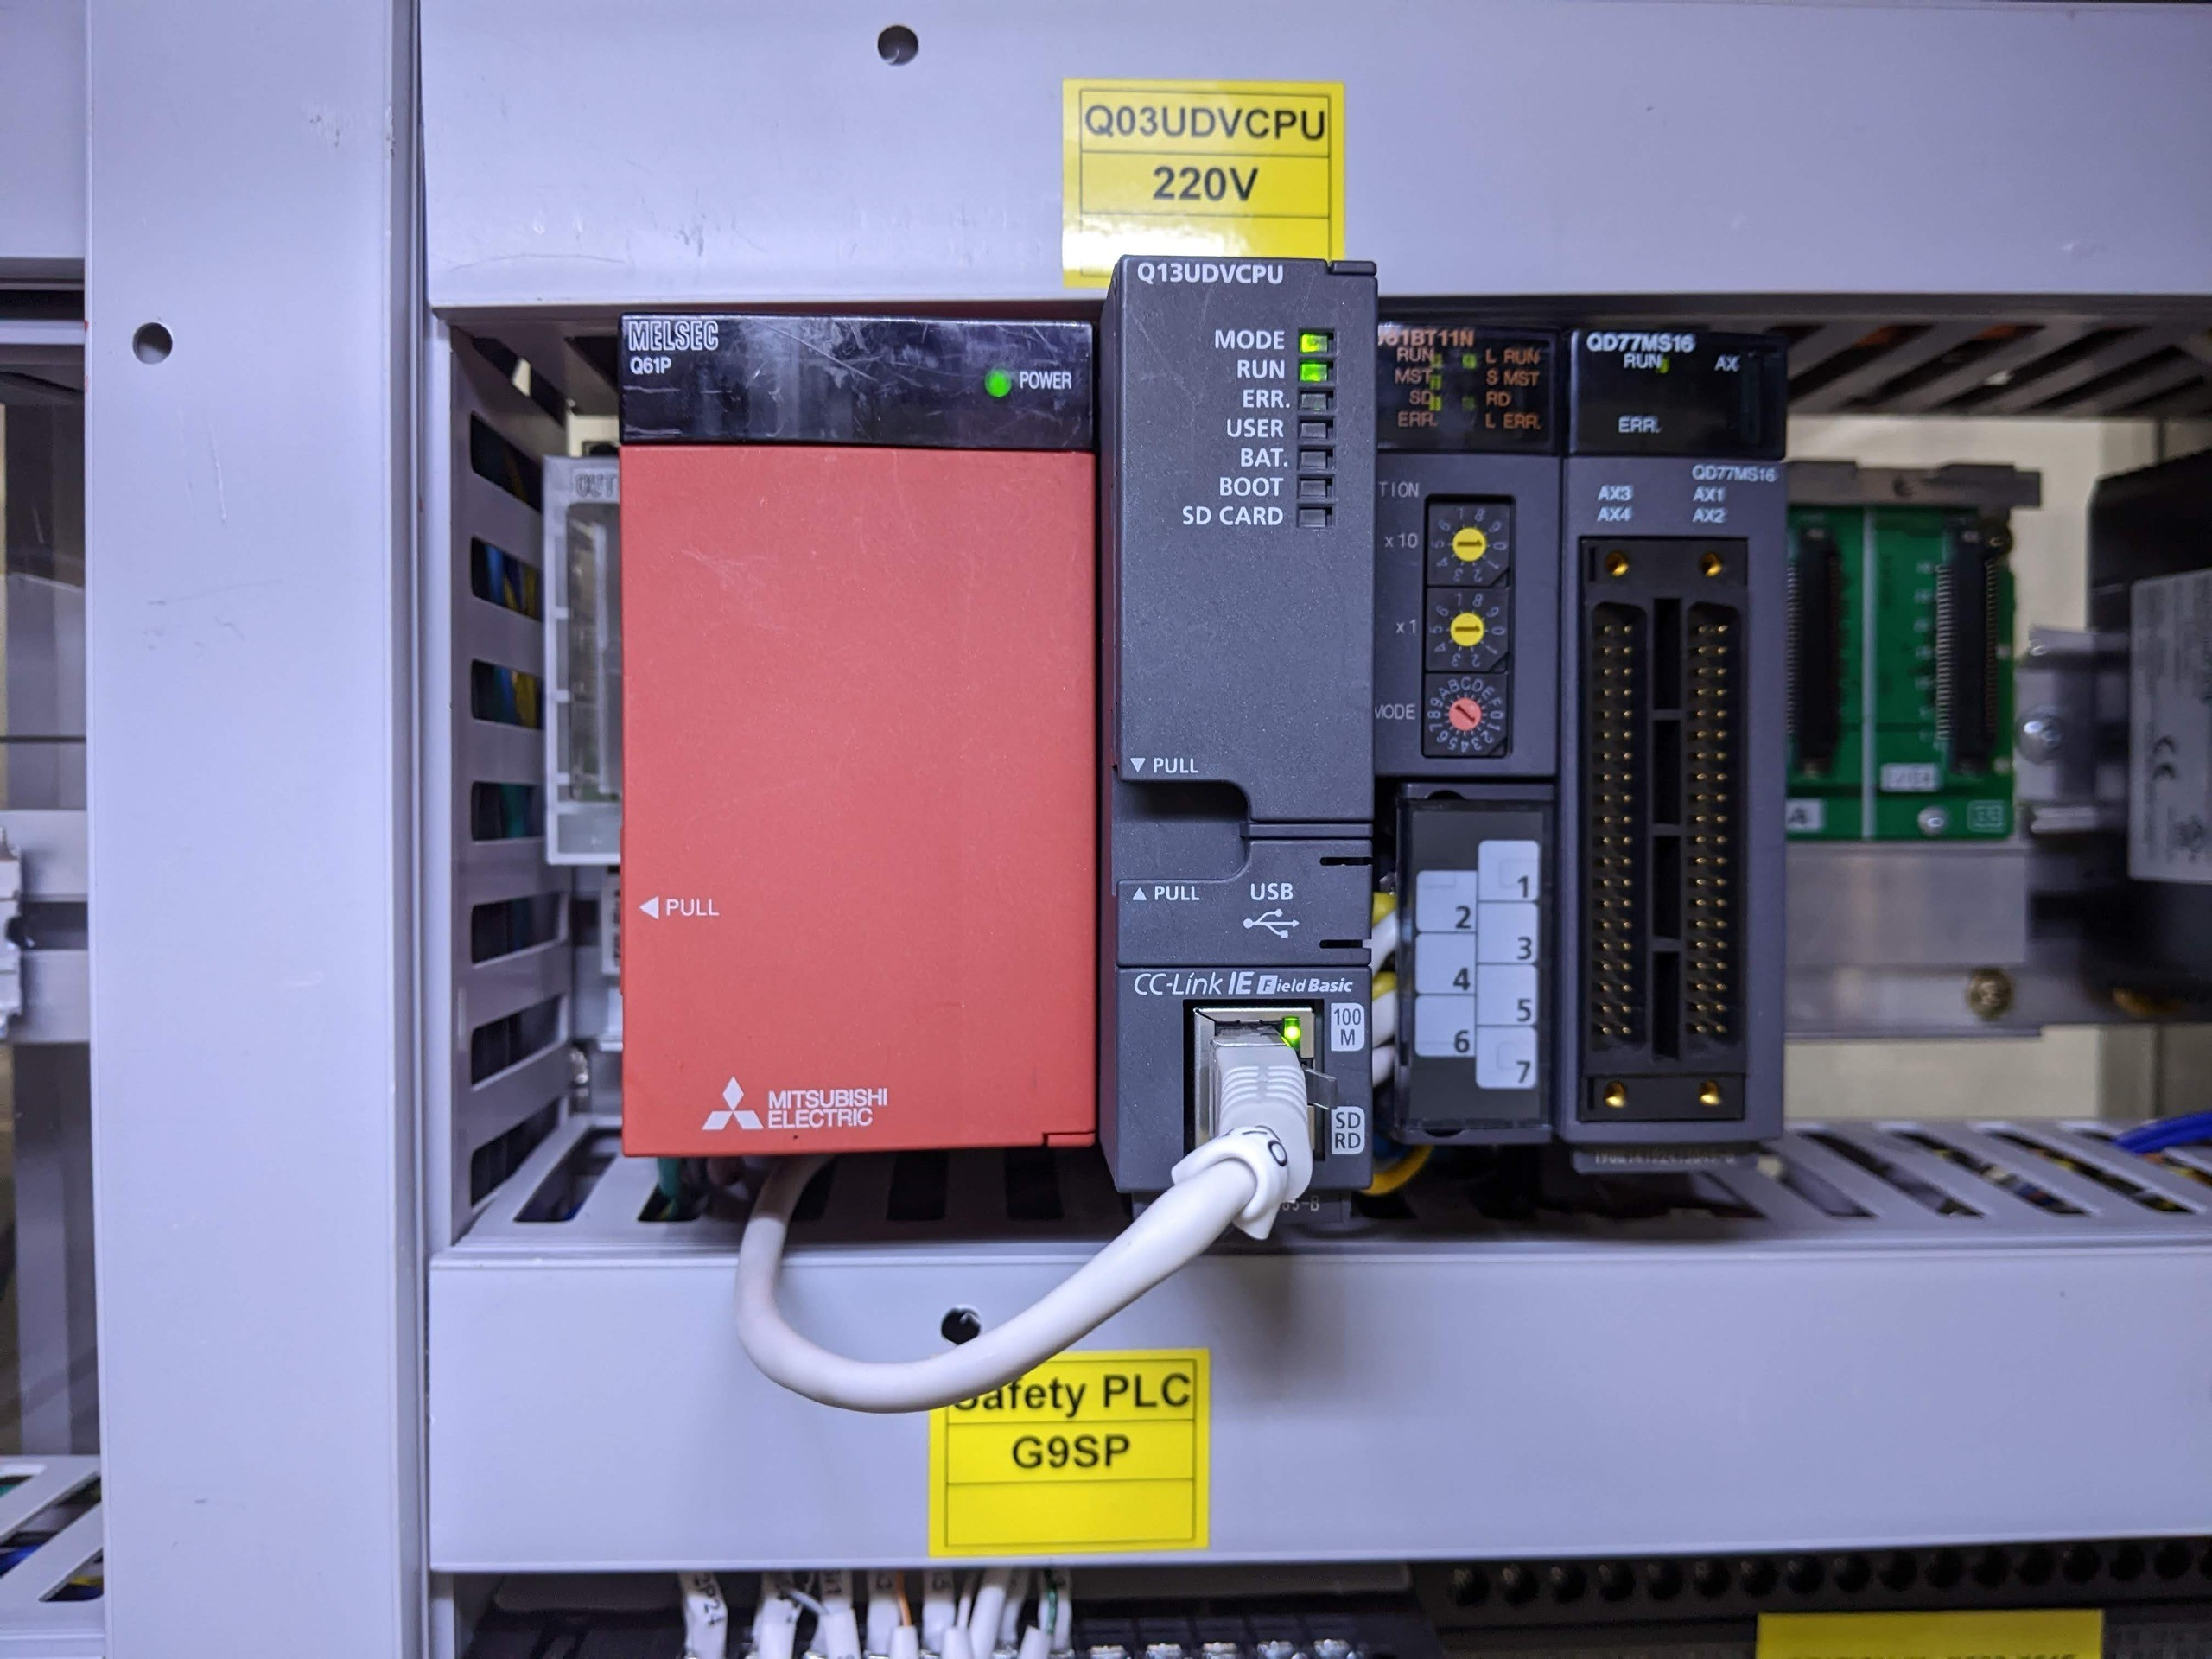
\includegraphics[width=0.75\linewidth]{figures/Chapter3/phancung.png}
    \caption{Thiết lập phần cứng}
    \label{c3:hardware}
    \end{figure}

    
    \begin{figure}[H]
        \centering
        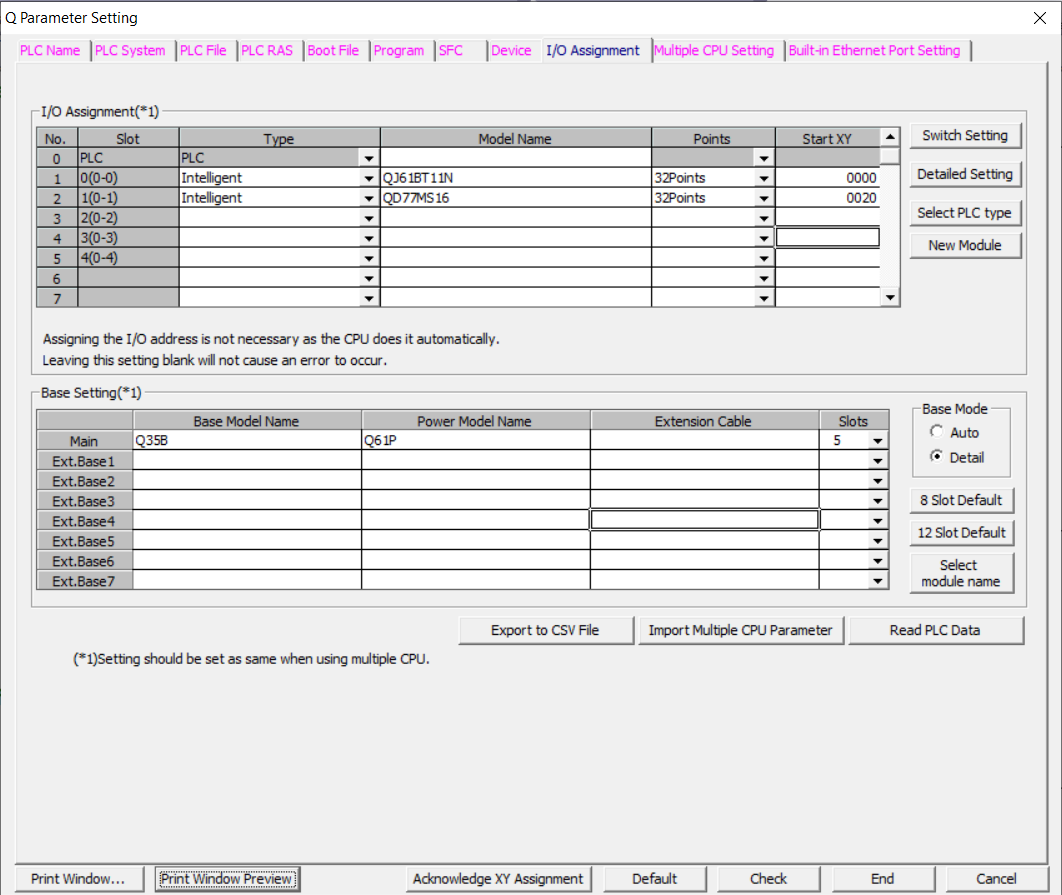
\includegraphics[width=0.75\linewidth]{figures/Chapter3/io.png}
        \caption{IO Assignment}
        \label{c3:io}
    \end{figure}

    \item Cấu hình giao tiếp/kết nối giữa PLC với GX Works2 (PC Side) như Hình \ref{c3:ethernet}. Bao gồm thiết lập IP cho PLC, giao thức MC Protocol.
    \begin{figure}[H]
        \centering
        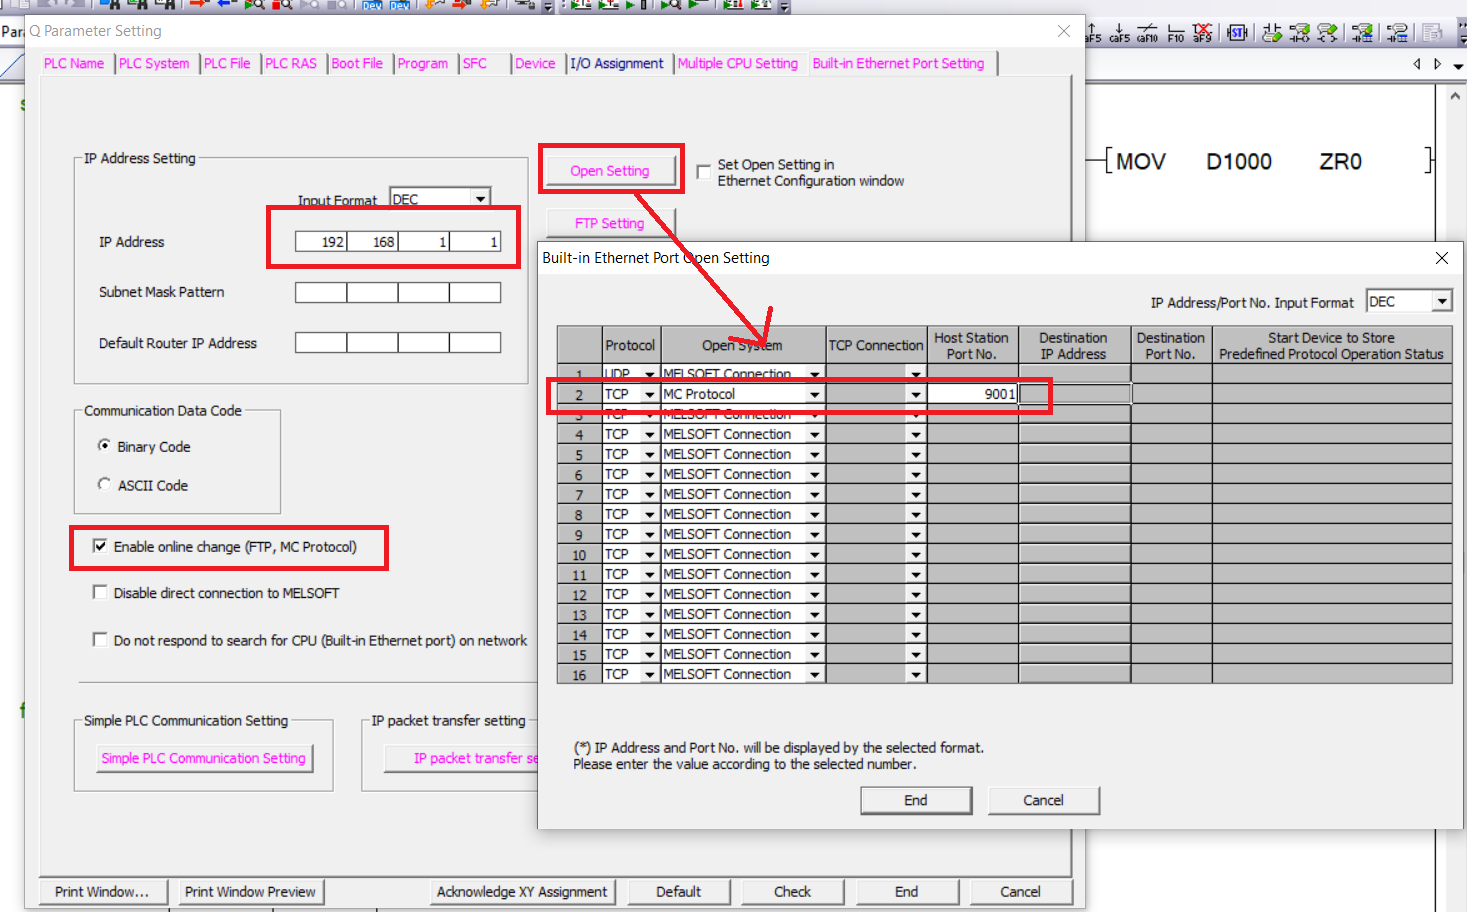
\includegraphics[width=0.75\linewidth]{figures/Chapter3/ethernet.png}
        \caption{Thiết lập kết nối Ethernet}
        \label{c3:ethernet}
    \end{figure}  
\end{enumerate}
Sau khi kết thúc thiết lập, bấm End để lưu thiết lập.

 \subsection{Cấu hình CC-Link giao tiếp giữa PLC và các CC-Link Station}

Để có thể kết nối các trạm với PLC qua CC-Link cần thiết lập cả phần cứng và phần mềm.
Cần cấu hình hai thông số quan trọng là phiên bản CC-Link (Ver 2 hoặc Ver 1), tốc độ truyền (khoảng cách càng gần thì tốc độ càng cao), số thứ tự Station cho từng trạm (cả Remote IO và Remote Device).

\begin{enumerate}
    \item \textbf{Trạm I/O}: Cấu hình các trạm IO là Remote IO Station. 
    Hình minh họa phần cứng của Remote IO giống như Hình \ref{c3:remoteio}. Có hai thành phần quan trọng là công tắc định địa chỉ Station (3) và công tắc định tốc độ giao tiếp (2). Cần phải điều khiển sao cho tốc độ đúng với tốc độ hệ thống và địa chỉ phù hợp, không bị trùng với các trạm khác.
        
    \begin{figure}[H]
        \centering
        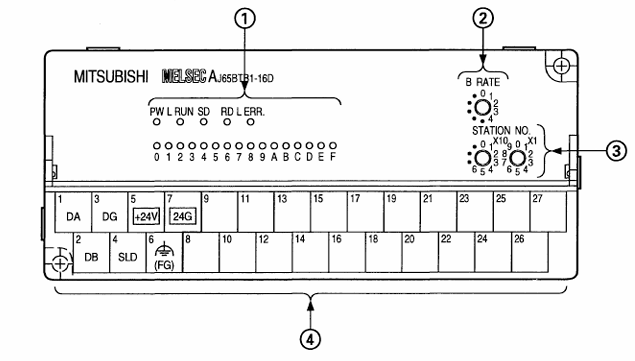
\includegraphics[width=0.75\linewidth]{figures/Chapter3/remote-io.png}
        \caption{Phần cứng Remote IO}
        \label{c3:remoteio}
    \end{figure}  

    \item \textbf{Robot Hyundai}: Cấu hình robot là Remote Device Station.
    Để có thể giao tiếp với mạng CC-Link, cần gắn thêm board giao tiếp CC-Link BD570 vào bộ điều khiển, minh họa như Hình\ref{c3:cc1}.
    \begin{figure}[H]
        \centering
        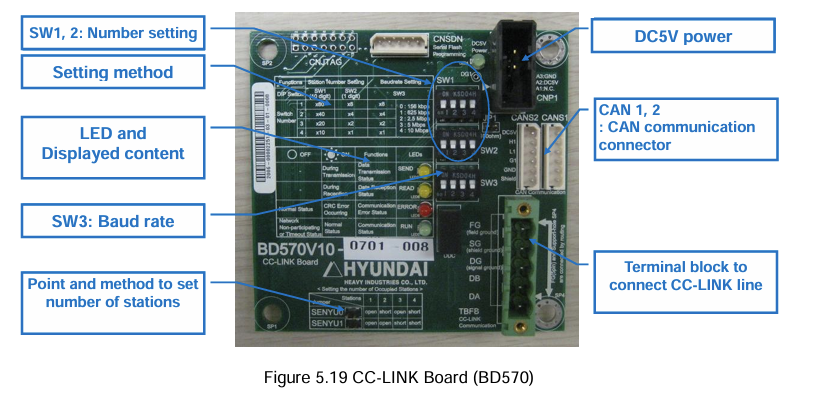
\includegraphics[width=1\linewidth]{figures/Chapter3/h-cc.png}
        \caption{Board CC-Link}
        \label{c3:cc1}
    \end{figure}
    Gắn board CC-Link vào bộ điều khiển, sau đó thiết lập vị trí trạm và tốc độ truyền bằng các switch có trên board.
    Sau khi bật nguồn bộ điều khiển, thông tin về giao tiếp CC-Link được hiển thị bằng Teach pendant (Hình \ref{c3:cc2}).
    \begin{figure}[H]
        \centering
        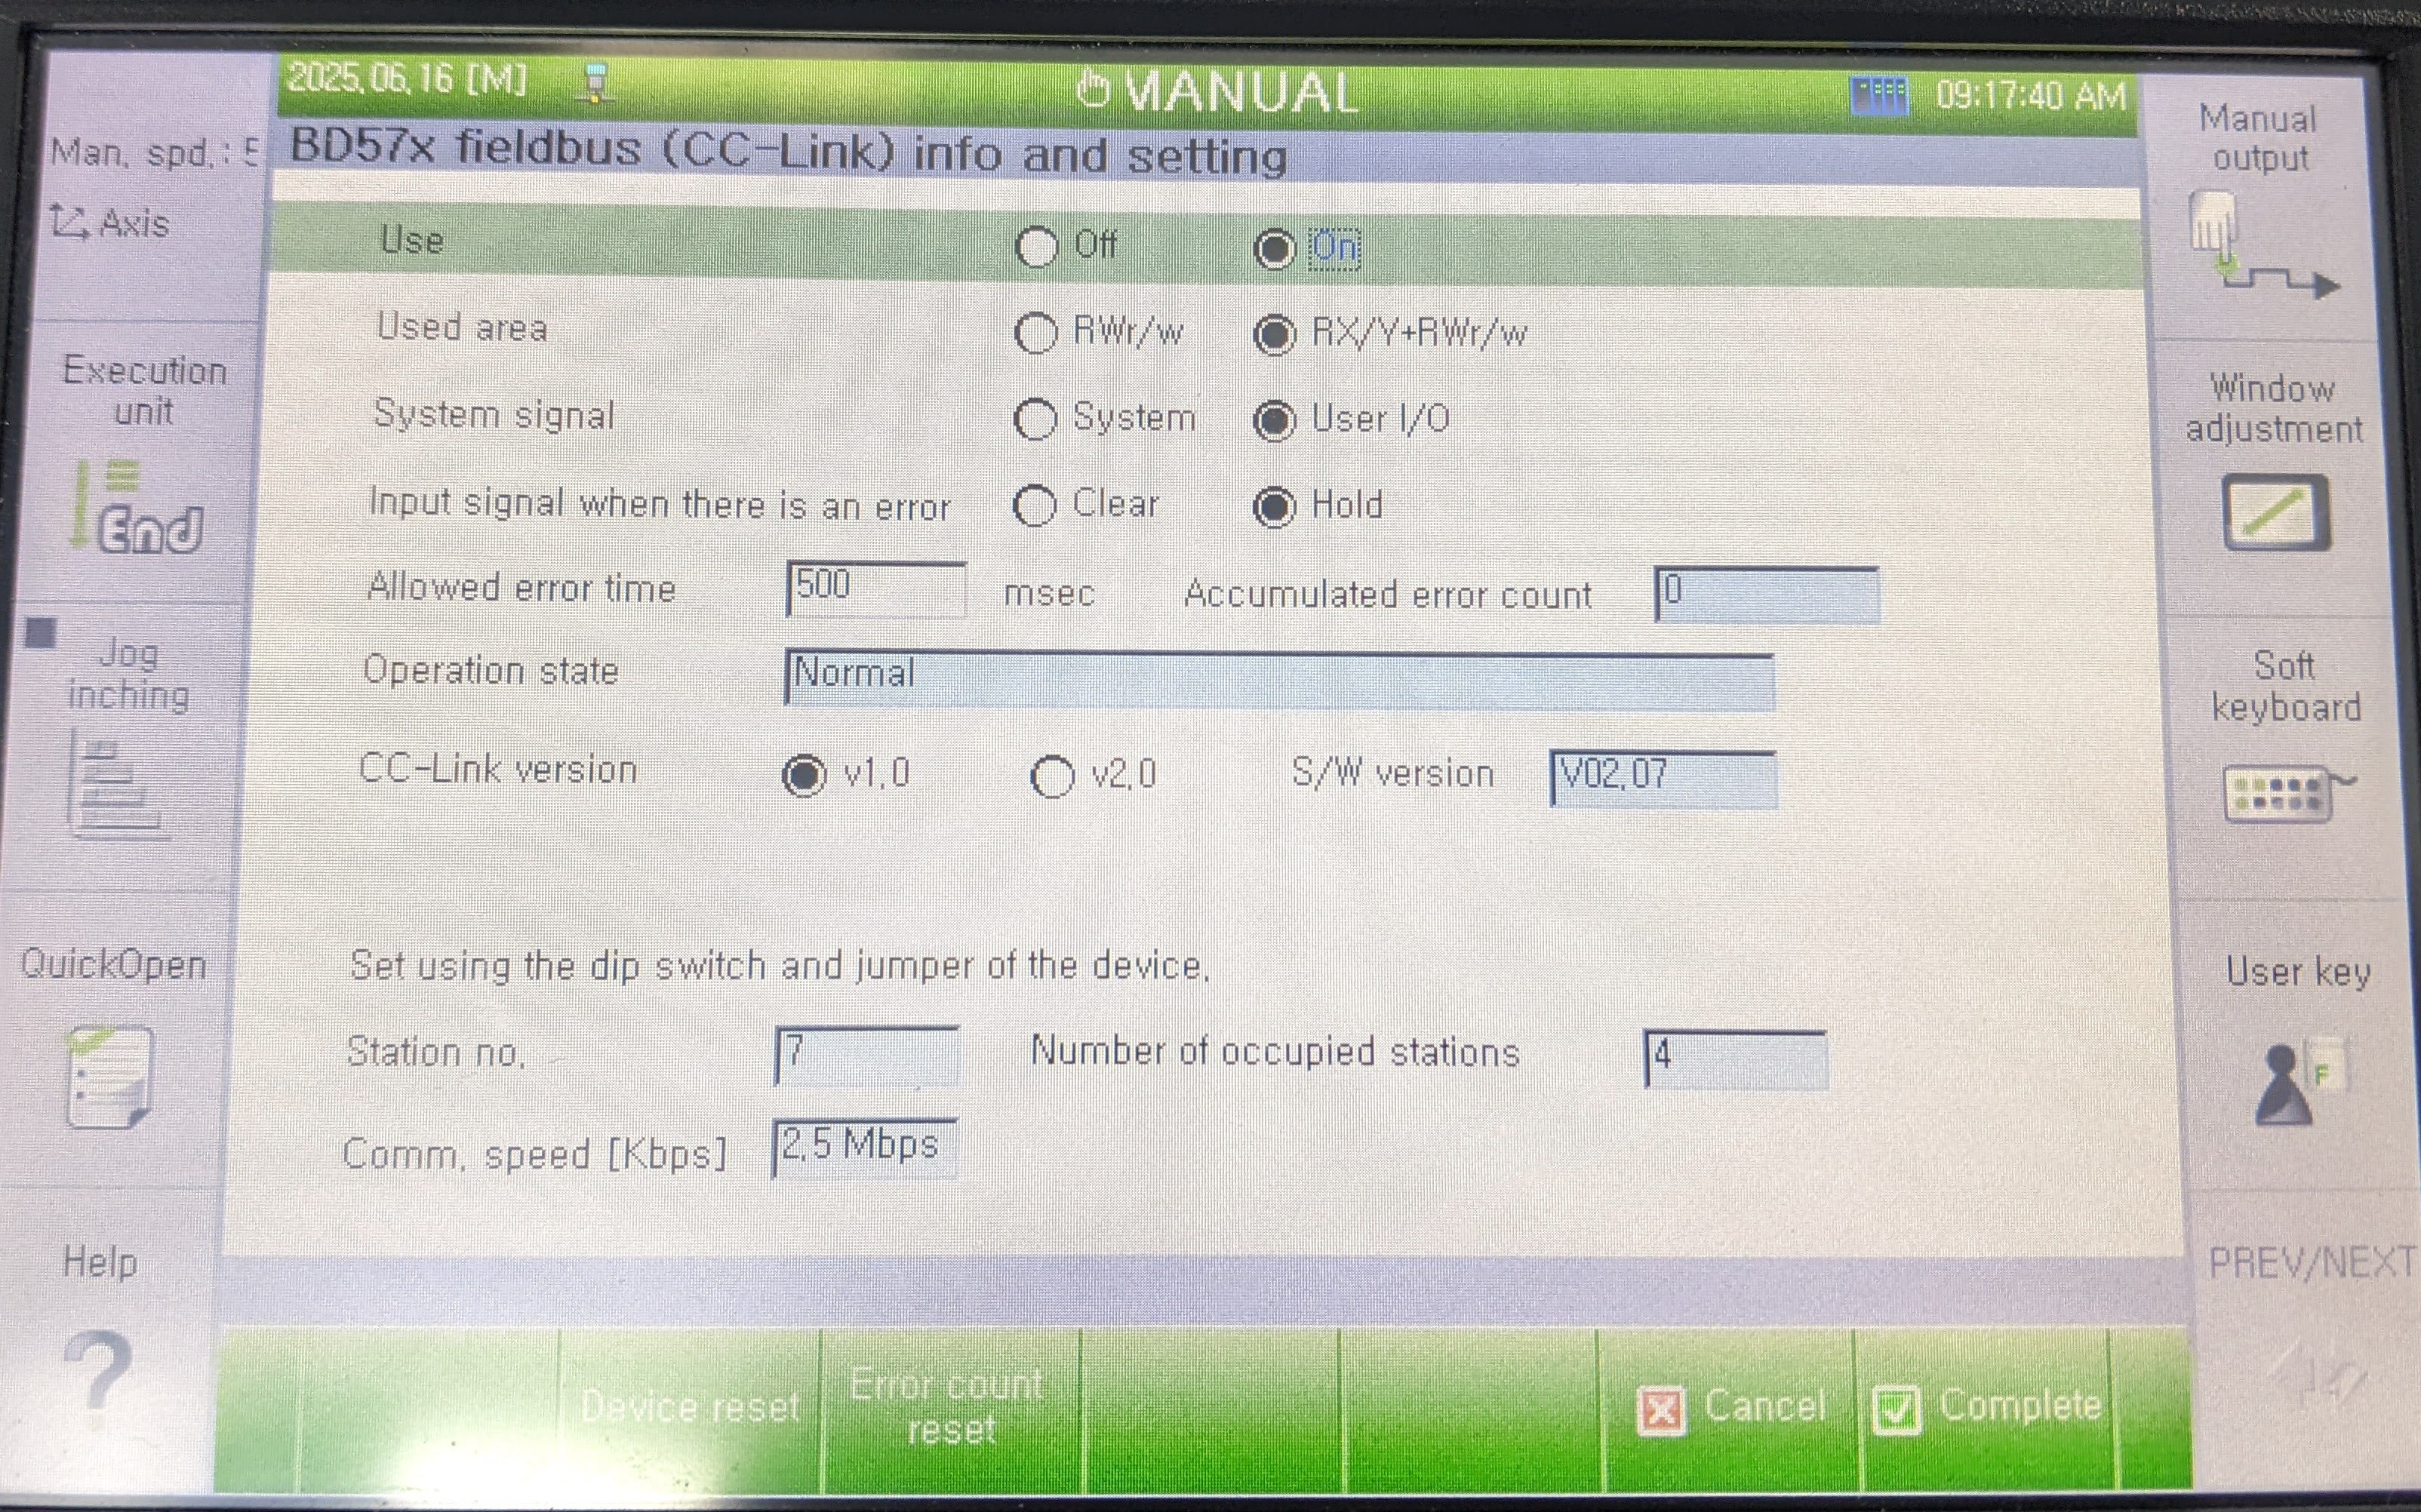
\includegraphics[width=1\linewidth]{figures/Chapter3/h-cc2.jpg}
        \caption{Thiết lập CC-Link Robot Hyundai}
        \label{c3:cc2}
    \end{figure}
    Thông số cấu hình CC-Link của Robot Hyundai:
    \newline
    \begin{tabular}{lc}
        \toprule
        \midrule
        Station no. & 7 \\
        Number of occupied stations & 4 \\
        Communication speed & 2.5 Mbps \\
        CC-Link version & v1.0 \\
        \bottomrule
    \end{tabular}

 Sau khi cấu hình xong, dữ liệu từ CC-Link được hiển thị tại 
\texttt{F1:Service} $\rightarrow$ 
\texttt{1:Monitoring} $\rightarrow$ 
\texttt{3:Field bus signal} $\rightarrow$ 
\texttt{9/10:FB5 Field bus input/output}.



    \newpage
    \item \textbf{Robot Yaskawa}: Cấu hình robot là Remote Device Station. 
    Để có thể kết nối Robot với PLC qua CC-Link giúp truyền nhận tín hiệu In/Out và Register, cần phải lắp đặt phần cứng là CCS-PCIE Board (Hình \ref{c3:yas2})vào bộ điều khiển của Robot YRC1000micro.
    \begin{figure}[H]
        \centering
        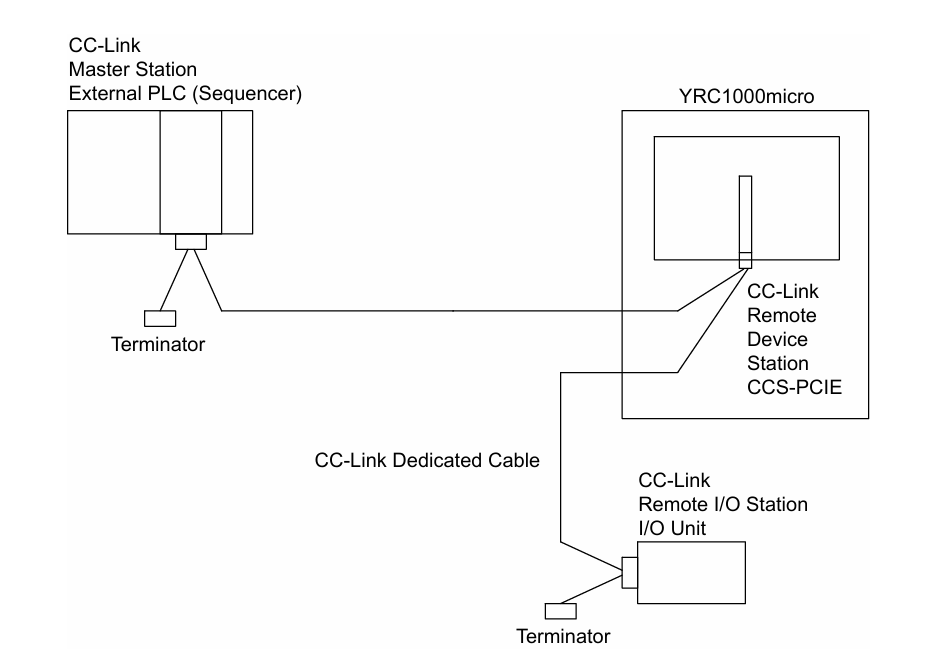
\includegraphics[width=0.8\linewidth]{figures/Chapter3/yas1.png}
        \caption{Kết nối CC-Link giữa Robot Yaskawa và PLC}
        \label{c3:yas1}
    \end{figure}
    

    \begin{figure}[H]
        \centering
        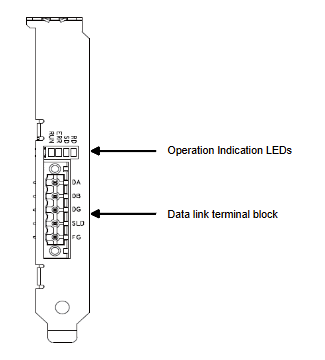
\includegraphics[width=0.5\linewidth]{figures/Chapter3/y-cc1.png}
        \caption{Board CCS-PCIE}
        \label{c3:yas2}
    \end{figure}

    Thiết lập giao tiếp CC-Link cần vào Maintenance Mode: nhấn \texttt{[MAIN MENU]} trong khi bật nguồn YRC1000micro.  
    Sau đó thiết lập thông tin cho Board CCS-PCIE như dưới:
    \begin{figure}[H]
        \centering
        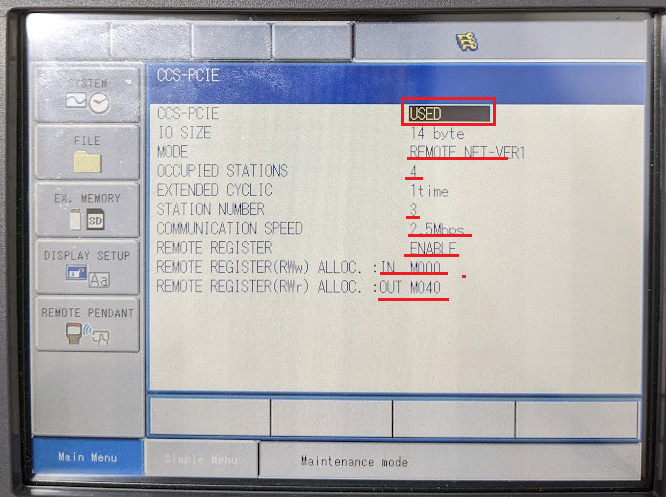
\includegraphics[width=1\linewidth]{figures/Chapter3/cclink1.png}
        \caption{Thiết lập CC-Link Robot Yaskawa}
        \label{c3:yas3}
    \end{figure}

    Thông số cấu hình CC-Link của Robot Yaskawa:
    \newline
        \begin{tabular}{lc}
            \toprule
            \midrule
            Station no. & 3 \\
            Number of occupied stations & 4 \\
            Communication speed & 2.5 Mbps \\
            CC-Link version & v1.0 \\
            IO Size & 14 bytes \\
            \bottomrule
        \end{tabular}

    Ấn \texttt{[ENTER]} đến màn hình \textit{EXTERNAL IO SETUP}:
    \begin{figure}[H]
        \centering
        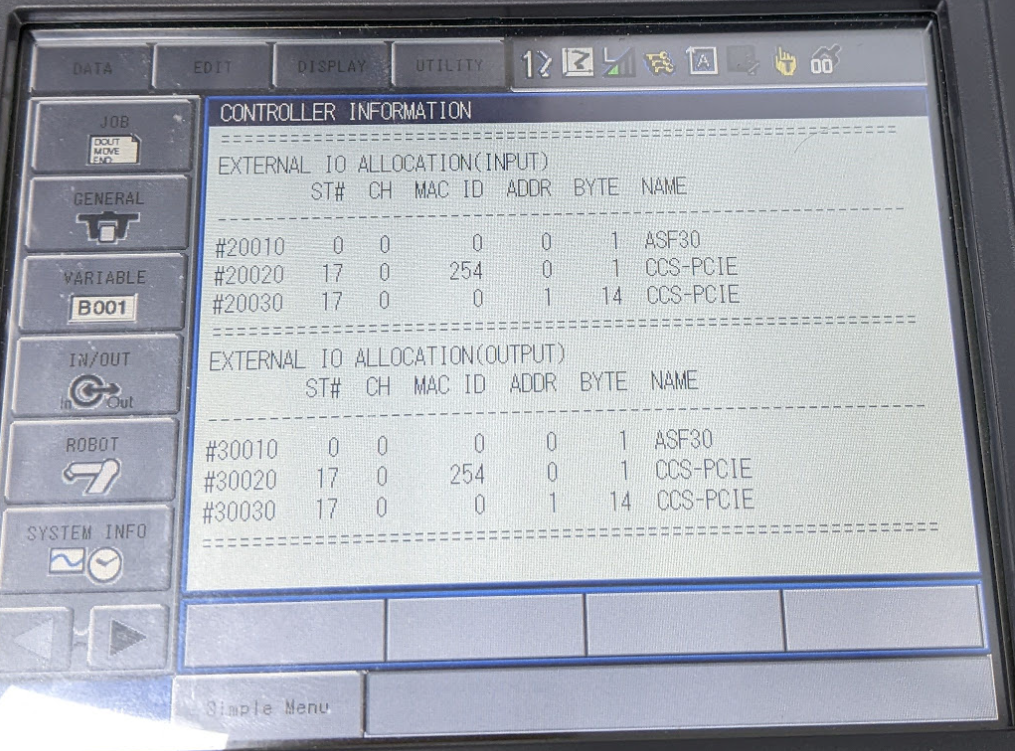
\includegraphics[width=1\linewidth]{figures/Chapter3/y-cc3.png}
        \caption{Controller Information}
        \label{c3:yas4}
    \end{figure}

    Hệ thống có ba loại dữ liệu vào/ra như sau:

    \begin{enumerate}
        \item \textbf{Dữ liệu từ board ASF30}:
        \begin{itemize}
            \item 8-bit input: \#20010–\#20017
            \item 8-bit output: \#30010–\#30017
        \end{itemize}

        \item \textbf{Dữ liệu trạng thái từ board CCS-PCIE}:
        \begin{itemize}
            \item 8-bit input: \#20020–\#20027
            \item 8-bit output: \#30020–\#30027
        \end{itemize}

        \item \textbf{Dữ liệu qua mạng CC-Link}:
        \begin{itemize}
            \item 14-byte input: \#20030–\#20167
            \item 14-byte output: \#30030–\#30167
        \end{itemize}
    \end{enumerate}

    Sau khi thiết lập dữ liệu từ CC-Link sang Robot, có thể kiểm tra tại  
    \texttt{[MAIN MENU]} $\rightarrow$ \texttt{IN/OUT} $\rightarrow$ \texttt{EXTERNAL INPUT/OUTPUT}.

    Để có thể sử dụng dữ liệu IO từ \texttt{EXTERNAL INPUT/OUTPUT} khi lập trình Robot cần chuyển vào \texttt{GENERAL PURPOSE INPUT/OUTPUT} \cite{YaskawaYRC1000microConcurrentIO} bằng cách sử dụng Ladder Program \cite{YaskawaYRC1000microOperatorManual}.

    \begin{figure}[H]
        \centering
        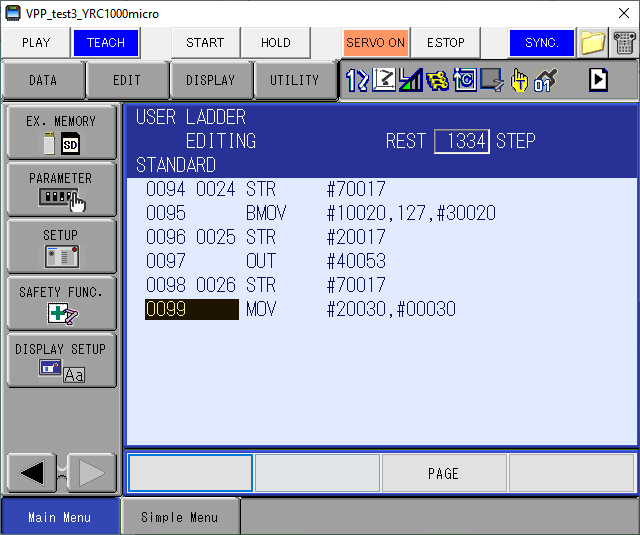
\includegraphics[width=1\linewidth]{figures/Chapter3/yas4.png}
        \caption{Ladder Program}
        \label{c3:yas5}
    \end{figure}

    \begin{figure}[H]
        \centering
        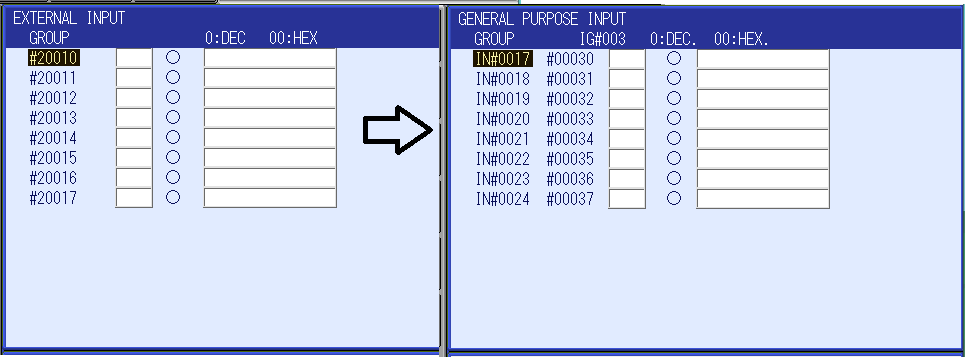
\includegraphics[width=1\linewidth]{figures/Chapter3/yas5.png}
        \caption{Dữ liệu chuyển vào GP INPUT/OUTPUT}
        \label{c3:yas6}
    \end{figure}

    Ví dụ: tại dòng 98–99, \texttt{\#20030 – \#20037} của \texttt{External Input} được chuyển vào \texttt{\#00030–\#00037} của \texttt{General Purpose Input}.

    \item \textbf{Cấu hình PLC là Master}

    Trong mục thiết lập tham số CC-Link của GX-Works2, cấu hình như sau:

    Thiết lập thông tin trạm Master (Hình \ref{c3:plc1} và Hình \ref{c3:plc2})

    \begin{figure}[H]
        \centering
        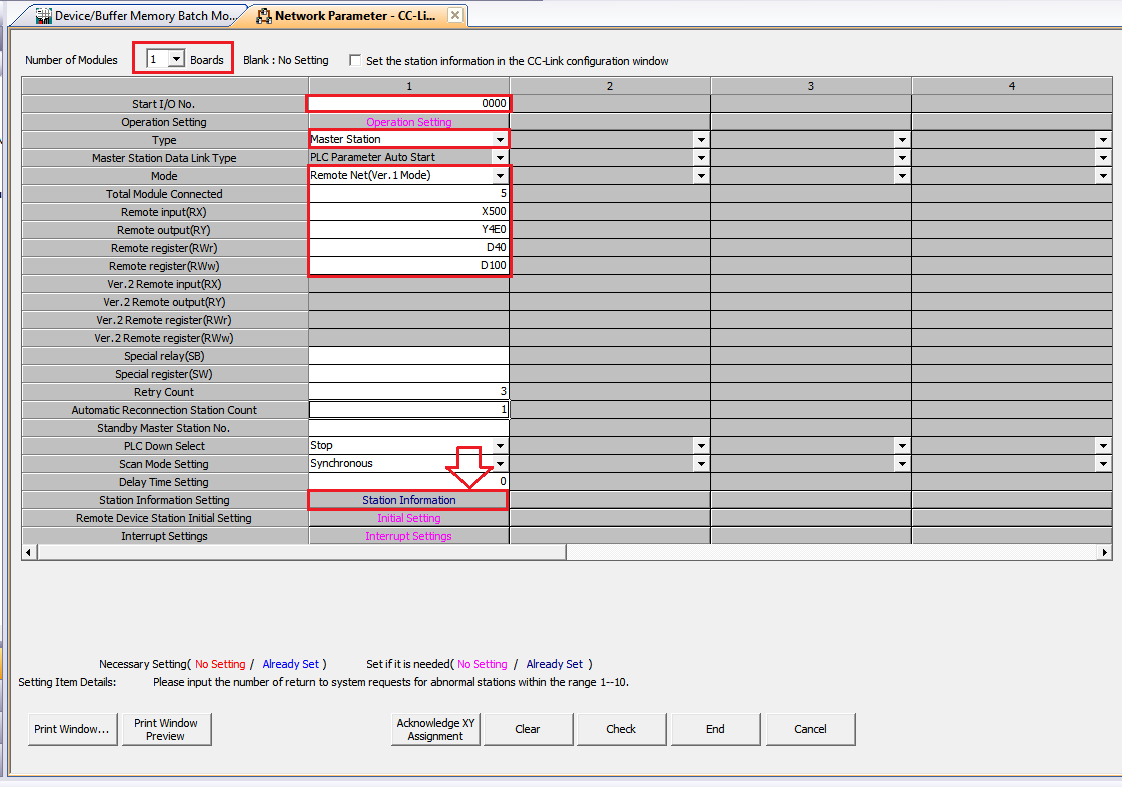
\includegraphics[width=0.9\linewidth]{figures/Chapter3/plc-cc1.png}
        \caption{Master Station}
        \label{c3:plc1}
    \end{figure}

    \begin{figure}[H]
        \centering
        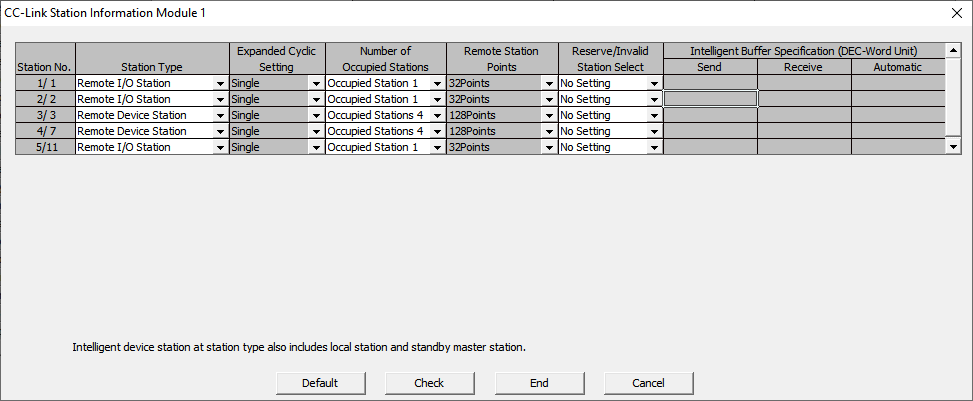
\includegraphics[width=1\linewidth]{figures/Chapter3/plc-cc2.png}
        \caption{Master Station Setup}
        \label{c3:plc2}
    \end{figure}

    \begin{figure}[H]
        \centering
        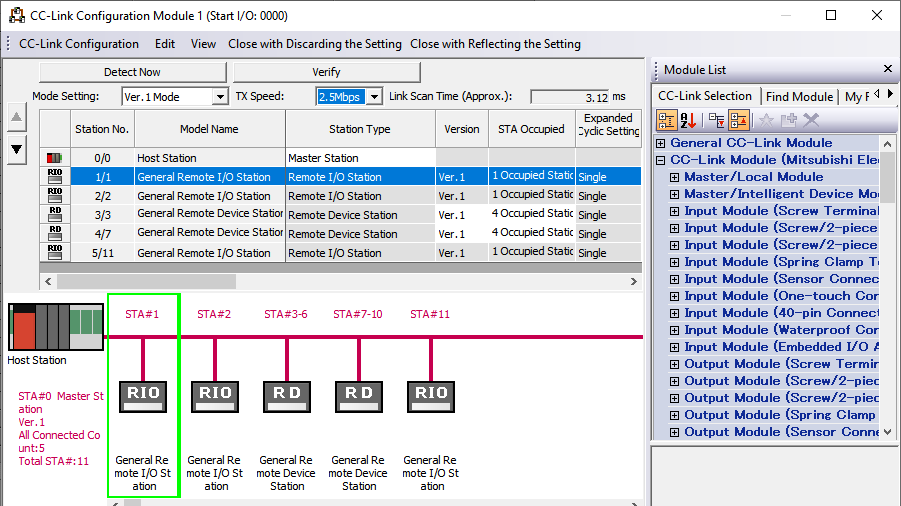
\includegraphics[width=1\linewidth]{figures/Chapter3/plc-cc3.png}
        \caption{CC-Link Speed}
        \label{c3:plc3}
    \end{figure}

    Sau khi thiết lập xong Master, thu được kết quả:

    \begin{itemize}
        \item Station \#1: AJ65SBTB1-32D
        \item Station \#2: AJ65SBTB1-32T1
        \item Station \#3: Robot Yaskawa (4 trạm)
        \item Station \#4: Robot Hyundai (4 trạm)
        \item Station \#5: AJ65SBT1-16DT1
    \end{itemize}

    Mỗi trạm chiếm:
    \begin{itemize}
        \item 32 bit tại Rx, Ry
        \item 4 word tại RWr, RWw
    \end{itemize}

    \begin{table}[h]
    \centering
    \begin{tabularx}{\textwidth}{|c|X|X|X|X|}
    \hline
    \textbf{Station} & \textbf{Rx} & \textbf{Ry} & \textbf{RWr} & \textbf{RWw} \\ \hline
    \#1 & X500--X51F & Y4E0--Y4FF & D40--D43 & D100--D103 \\ \hline
    \#2 & X520--X53F & Y500--Y51F & D44--D47 & D104--D107 \\ \hline
    \#3 & X540--X5BF & Y520--Y59F & D48--D63 & D108--D123 \\ \hline
    \#4 & X5C0--X63F & Y5A0--Y61F & D64--D79 & D124--D139 \\ \hline
    \#5 & X640--X65F & Y620--Y63F & D80--D83 & D140--D143 \\ \hline
    \end{tabularx}
    \caption{Bảng phân phối bit/word CC-Link}
    \label{tab:cclink}
    \end{table}


\end{enumerate}
%=------------------------------------------------------------------------------
\subsection{Cấu hình KepserverEX làm server OPC UA}
Kết nối KepserverEX với PLC qua card mạng của máy tính. Giao thức được chọn và sử dụng trong phần mềm GX-Works2 và phần mềm KepserverEX phải giống nhau để đảm bảo giao tiếp giữa OPC UA Server với PLC.

\begin{figure}[H]
        \centering
        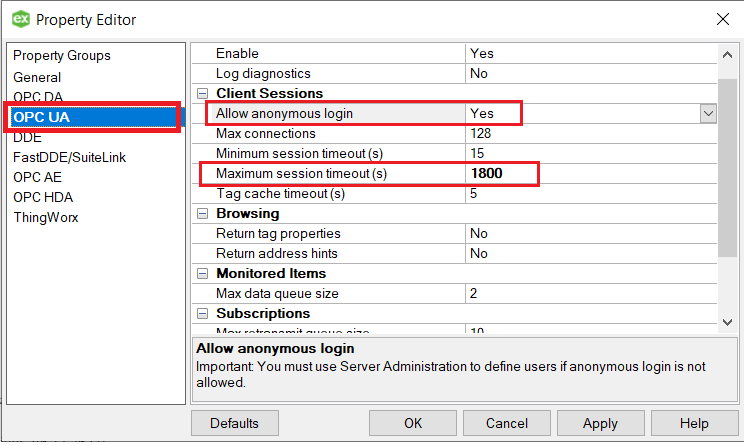
\includegraphics[width=1\linewidth]{figures/Chapter3/kepwareprj.png}
        \caption{Cấu hình Project Kepware}
        \label{c3:kepwareprj}
 \end{figure}

Cấu hình Project của Kepware như Hình \ref{c3:kepwareprj}, lưu ý bật cho phép truy cập ẩn danh.


\begin{figure}[H]
        \centering
        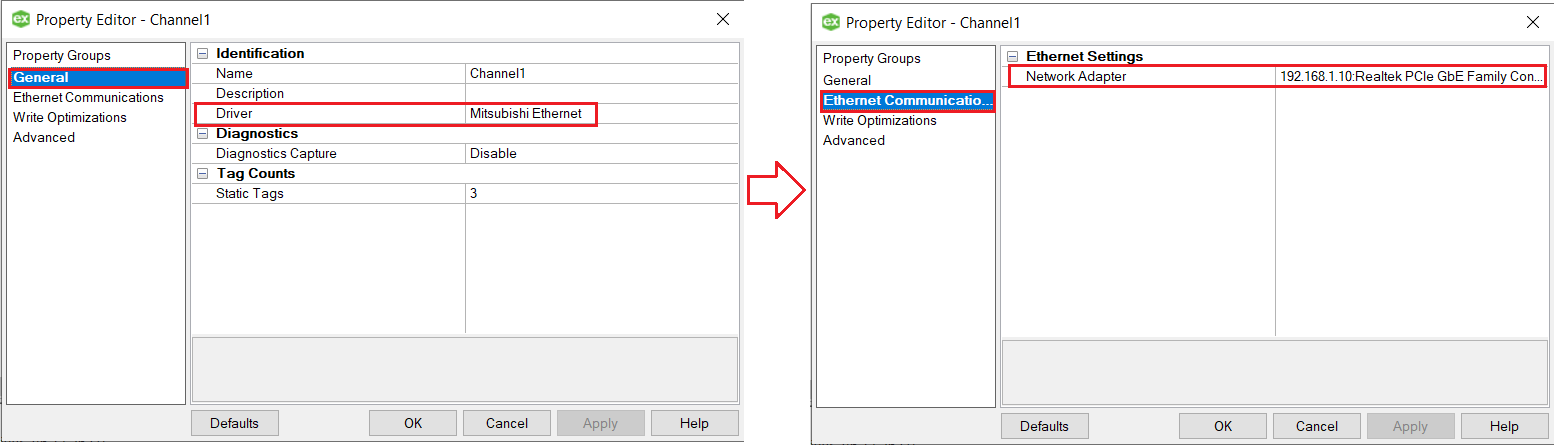
\includegraphics[width=1\linewidth]{figures/Chapter3/kepwarechannel.png}
        \caption{Cấu hình Channel}
        \label{c3:kepwarechannel}
 \end{figure}

Cấu hình Channel của Kepware project, lưu ý đúng với cổng mạng đang dùng của máy tính.

\begin{figure}[H]
        \centering
        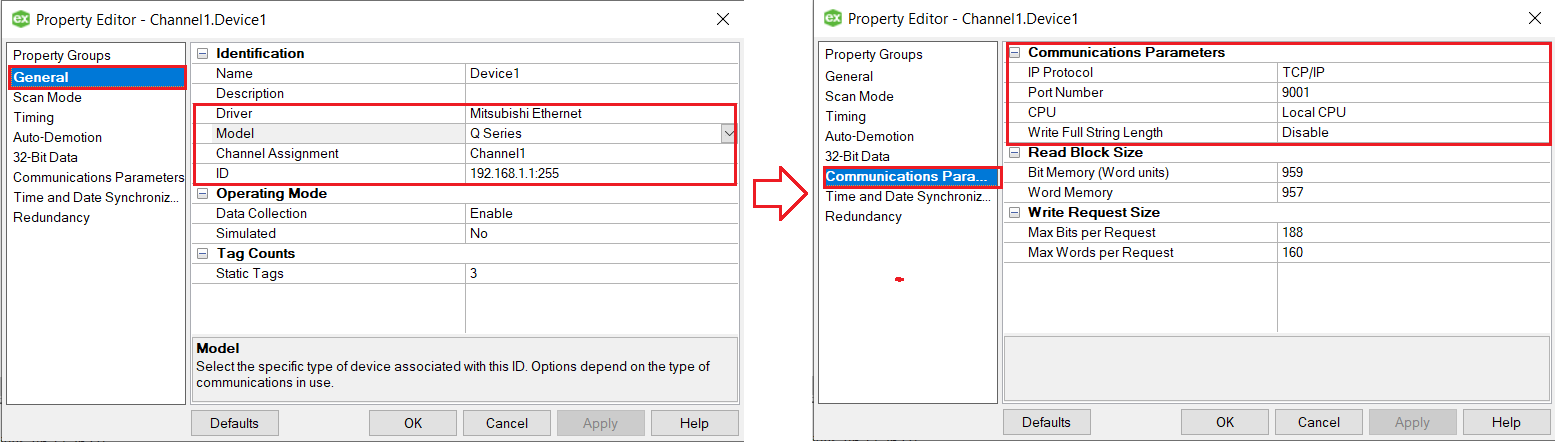
\includegraphics[width=1\linewidth]{figures/Chapter3/kepwaredevice.png}
        \caption{Cấu hình Device}
        \label{c3:kepwaredevice}
 \end{figure}

Cấu hình Device của Channel, lưu ý đúng với IP của PLC.

Tiếp theo cần tạo các Tag muốn sử dụng, tương ứng với địa chỉ các bit/word trong PLC


\subsection{Cấu hình GigE Camera Basler ac2500}
Kết nối Camera với máy tính qua cổng mạng IP, cần cấu hình IP của camera với IP của máy tính trong cùng lớp mạng (Hình \ref{c3:cameraip}).

\begin{figure}[H]
        \centering
        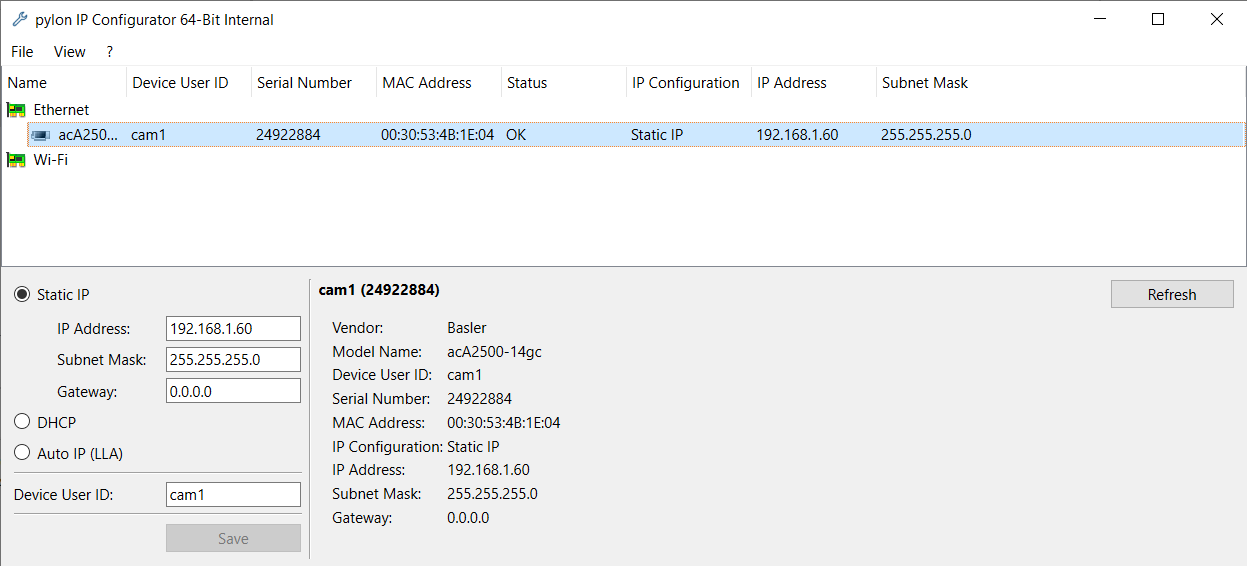
\includegraphics[width=1\linewidth]{figures/Chapter3/baslerip.png}
        \caption{Cấu hình IP camera}
        \label{c3:cameraip}
 \end{figure}

Tiếp theo là cấu hình thông số ảnh chụp như Gain, Gamma, Exposure time. Có thể sử dụng chức năng Automatic Image Adjustment (Hình \ref{c3:image}).

\begin{figure}[H]
        \centering
        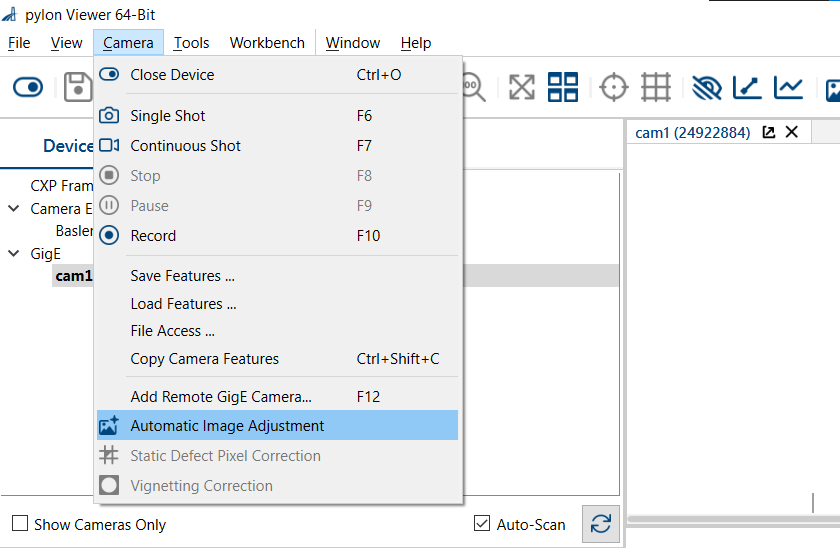
\includegraphics[width=1\linewidth]{figures/Chapter3/baslerauto.png}
        \caption{Cấu hình ảnh chụp}
        \label{c3:image}
 \end{figure}


% =======================
% PHẦN 3: XỬ LÝ ẢNH
% ======================= 


\section{Xây dựng hệ thống xử lý ảnh}

\subsection{Pipeline xử lý ảnh}
Hệ thống kiểm tra ngoại quan tự động (Automated Visual Inspection – AVI) vận hành thông qua một chuỗi các bước xử lý ảnh được tổ chức theo dạng pipeline nhằm đảm bảo quá trình kiểm tra diễn ra chính xác, ổn định và nhất quán. Pipeline xử lý ảnh của hệ thống có thể được mô tả qua các giai đoạn chính như sau:

\subsubsection{Thu nhận hình ảnh}
Ở giai đoạn đầu tiên, camera độ phân giải cao hoặc thiết bị ghi hình chuyên dụng được sử dụng để thu nhận ảnh hoặc video của sản phẩm. Chất lượng ảnh đầu vào phụ thuộc vào loại camera, ống kính, khoảng cách chụp và cấu hình hệ thống chiếu sáng. Đây là nguồn dữ liệu cơ bản phục vụ toàn bộ quá trình xử lý phía sau.

\subsubsection{Xử lý và tiền xử lý hình ảnh}
Sau khi thu nhận, hình ảnh được đưa vào các thuật toán xử lý nhằm tăng cường chất lượng, làm nổi bật đặc trưng quan trọng và giảm nhiễu. Các bước thường bao gồm:
\begin{itemize}
    \item Cân bằng sáng, tăng tương phản hoặc hiệu chỉnh màu.
    \item Lọc nhiễu và cải thiện độ nét.
    \item Chuẩn hóa kích thước, góc xoay hoặc cắt vùng quan tâm (ROI).
\end{itemize}
Giai đoạn này đảm bảo rằng hình ảnh đầu vào luôn đạt chất lượng ổn định để phục vụ nhận diện lỗi.

\subsubsection{Phân tích ảnh và nhận diện lỗi}
Ở bước này, hệ thống áp dụng các thuật toán xử lý ảnh nâng cao và mô hình học máy để:
\begin{itemize}
    \item Trích xuất đặc trưng của sản phẩm.
    \item Phát hiện các bất thường hoặc khuyết tật như vết nứt, thiếu linh kiện, sai lệch vị trí, biến dạng hình học.
    \item So sánh với hình mẫu hoặc tiêu chuẩn kỹ thuật đã thiết lập.
\end{itemize}
Thuật toán AI và machine learning giúp hệ thống thích nghi với biến động trong môi trường sản xuất, từ đó cải thiện độ chính xác theo thời gian.

\subsubsection{Ra quyết định}
Dựa trên các tiêu chí chất lượng đã định nghĩa trước, hệ thống phân loại sản phẩm thành hai nhóm: đạt yêu cầu (OK) hoặc không đạt (NG). Việc ra quyết định được tự động hóa và đảm bảo tính khách quan, loại bỏ hoàn toàn yếu tố chủ quan của con người.

\subsubsection{Phản hồi và lưu trữ dữ liệu}
Kết quả kiểm tra được ghi nhận và phản hồi trực tiếp đến hệ thống sản xuất để thực hiện các hành động kịp thời như loại bỏ sản phẩm lỗi hoặc điều chỉnh quy trình. Đồng thời, dữ liệu hình ảnh, log lỗi và thống kê được lưu trữ trên cơ sở dữ liệu cục bộ hoặc đám mây để phục vụ phân tích chất lượng, tối ưu hoá dây chuyền và truy vết trong sản xuất.

Pipeline trên giúp hệ thống AVI hoạt động mạch lạc, hiệu quả và có khả năng mở rộng theo yêu cầu thực tế của từng dây chuyền sản xuất.

\subsection{Train mô hình YOLO detect linh kiện SMD}

\subsubsection{Thu thập dữ liệu}
Ảnh được thu thập trực tiếp từ camera trong dây chuyền bằng cách chụp nhiều mẫu PCB ở nhiều điều kiện khác nhau: thay đổi độ sáng, vị trí, góc đặt bảng, và trạng thái linh kiện (đầy đủ hoặc lỗi). Mục tiêu là tạo bộ dữ liệu đa dạng, phản ánh đúng môi trường sản xuất thực tế để mô hình học sâu có khả năng tổng quát tốt.

\begin{figure}[H]
    \centering
    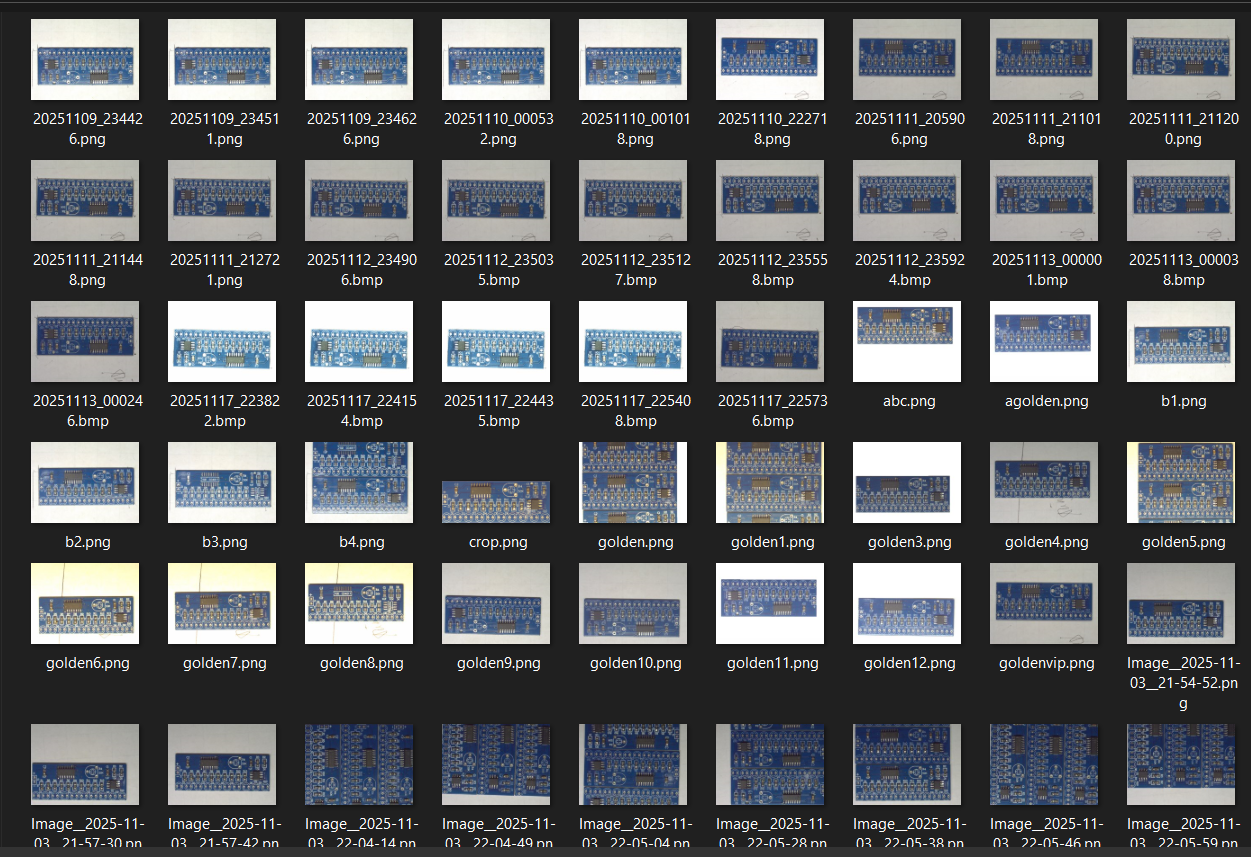
\includegraphics[width=0.75\linewidth]{figures/Chapter3/image11.png}
    \caption{Thu thập ảnh}
    \label{c3:acquistion}
\end{figure}

\subsubsection{Gán nhãn dữ liệu (Labeling)}
Sau khi thu thập, toàn bộ ảnh được đưa vào nền tảng Roboflow để thực hiện gán nhãn. Mỗi linh kiện SMD hoặc vùng lỗi trên PCB được bao quanh bằng bounding box và gán class tương ứng, chẳng hạn như \texttt{OK}, \texttt{Missing}, \texttt{Shifted}, \texttt{Wrong\_Orientation}, \ldots{} Việc gán nhãn được thực hiện thủ công nhằm đảm bảo độ chính xác, vì chất lượng nhãn có ảnh hưởng trực tiếp đến khả năng học của mô hình YOLO.

Roboflow hỗ trợ việc chuẩn hoá kích thước ảnh, tăng cường dữ liệu (augmentation) như xoay, thay đổi độ sáng, cắt, lật ảnh, giúp tăng độ đa dạng cho tập huấn luyện. Sau khi hoàn tất, bộ dữ liệu được export theo định dạng YOLO và sẵn sàng cho quá trình huấn luyện.
\begin{figure}[H]
    \centering
    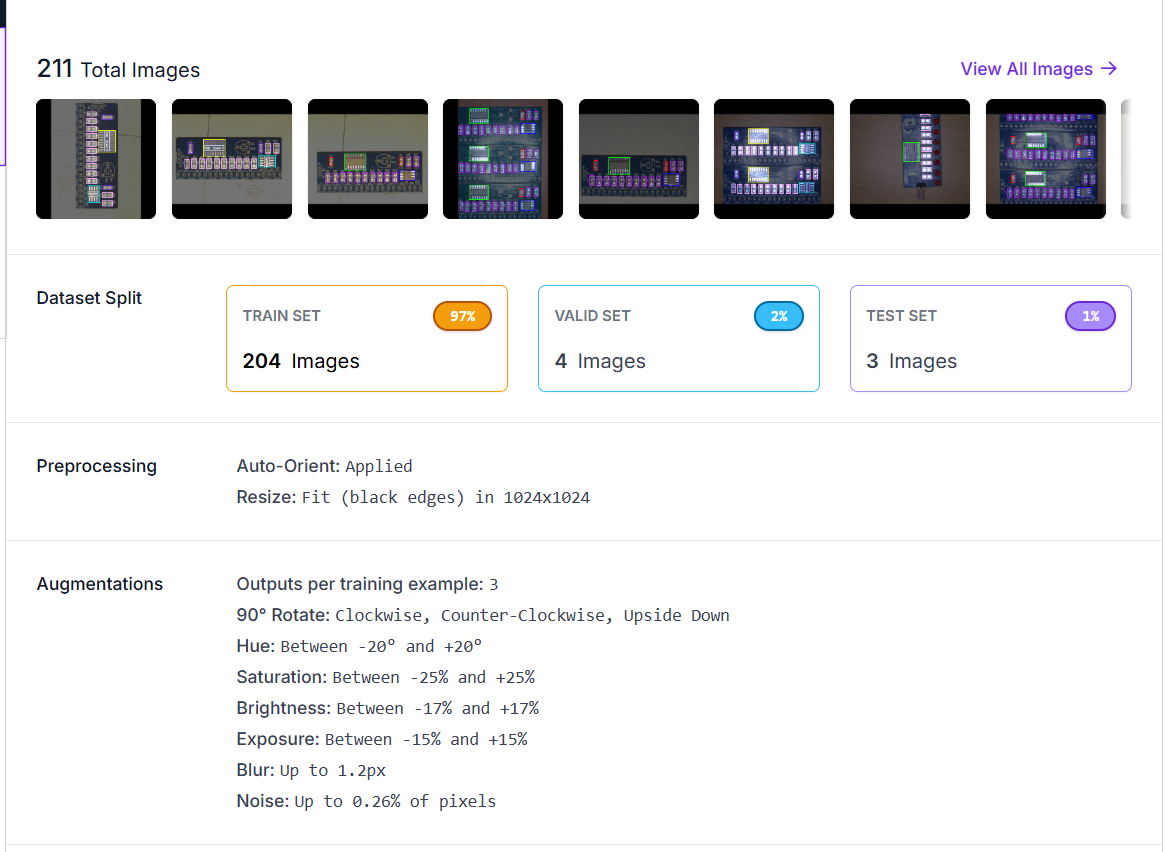
\includegraphics[width=0.75\linewidth]{figures/Chapter3/image12.png}
    \caption{Label ảnh bằng Roboflow}
    \label{c3:labeling}
\end{figure}

\subsubsection{Huấn luyện mô hình (Train model)}
Bộ dữ liệu sau khi export được đưa lên môi trường Google Colab để huấn luyện mô hình YOLO. Colab cung cấp GPU miễn phí, phù hợp cho huấn luyện nhanh các mô hình kích thước vừa.

Quy trình huấn luyện gồm các bước:
\begin{itemize}
    \item Upload bộ dữ liệu từ Roboflow vào Colab bằng API.
    \item Cấu hình file huấn luyện: đường dẫn dữ liệu, số lớp (classes), độ phân giải ảnh, batch size, và số epochs.
    \item Tiến hành huấn luyện và theo dõi các chỉ số: loss, precision, recall, mAP.
    \item Lưu lại \texttt{best.pt} sau khi huấn luyện, sử dụng cho giai đoạn suy luận (inference) trong hệ thống AVI.
\end{itemize}

Mô hình sau khi huấn luyện được tải xuống và đưa vào pipeline xử lý ảnh để thực hiện phát hiện linh kiện SMD trong thời gian gần thực.


\section{Thực nghiệm và đánh giá}

\subsection{Giao diện hệ thống}

Hệ thống AVI được triển khai với hai giao diện chính: giao diện ứng dụng AVI trên máy tính (Hình \ref{c4:application}) được viết bằng PyQt5 và giao diện HMI trên dây chuyền (Hình \ref{c4:hmi}). Giao diện AOI cho phép hiển thị kết quả quá trình xử lý ảnh, là ảnh sau khi đã xử lý xong các bước align, crop và YOLO detect, các hộp bao từ mô hình YOLO cũng như kết quả đánh giá OK/NG của từng linh kiện. Người vận hành có thể phóng to, thu nhỏ, xem log xử lý theo thời gian thực và lưu toàn bộ ảnh phục vụ mục đích truy vết. Bên cạnh đó, giao diện HMI được thiết kế đơn giản hơn, phục vụ công nhân sản xuất, hiển thị trạng thái các thành phần trong hệ thống như trạng thái băng tải, trạng thái robot, tín hiệu cảm biến, số lượng sản phẩm OK/NG và các nút điều khiển như Start, Stop và Reset. Hai giao diện kết hợp giúp việc vận hành và giám sát hệ thống trở nên trực quan và thuận tiện.

\begin{figure}[H]
    \centering
    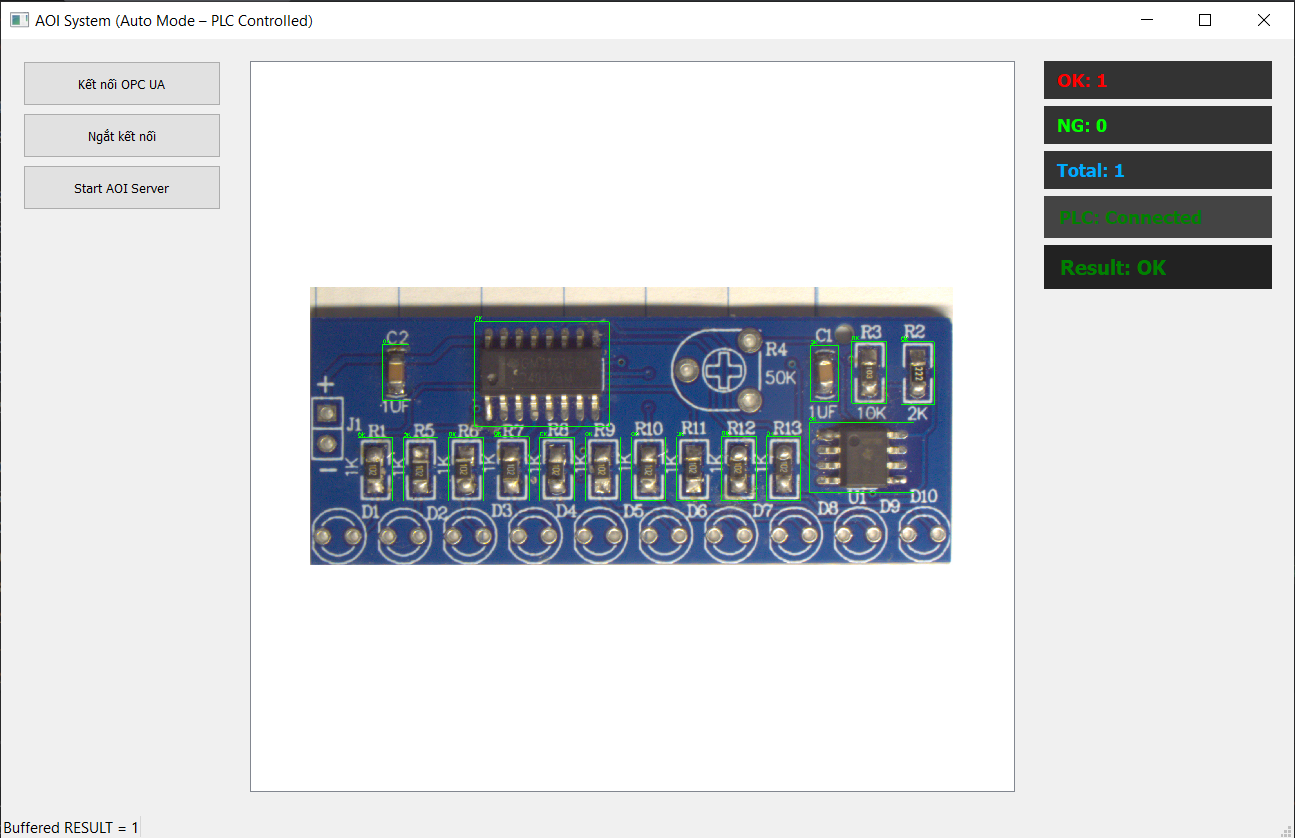
\includegraphics[width=1\linewidth]{figures/Chapter4/image1.png}
    \caption{Giao diện phần mềm AVI}
    \label{c4:application}
\end{figure}

\begin{figure}[H]
    \centering
    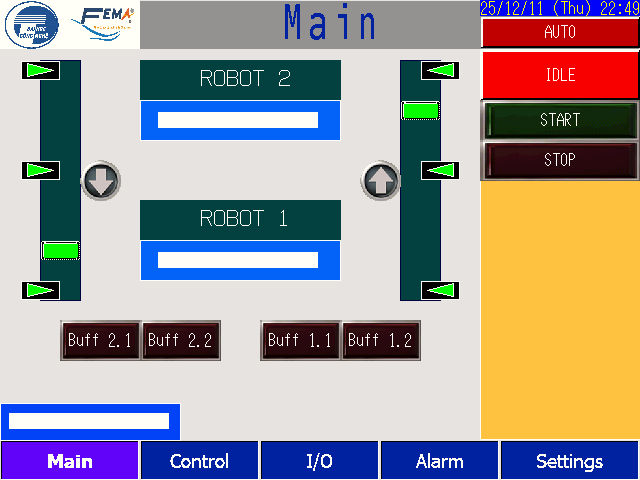
\includegraphics[width=0.8\linewidth]{figures/Chapter4/img2.jpg}
    \caption{Giao diện HMI}
    \label{c4:hmi}
\end{figure}


\begin{figure}[H]
    \centering
    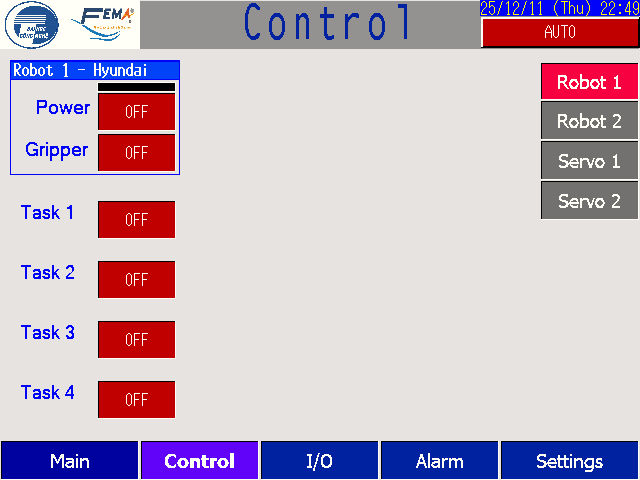
\includegraphics[width=0.48\linewidth]{figures/Chapter4/img1.jpg}
    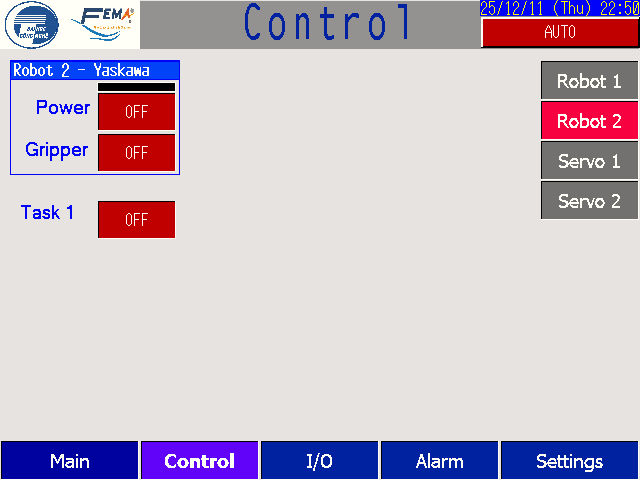
\includegraphics[width=0.48\linewidth]{figures/Chapter4/img3.jpg}
    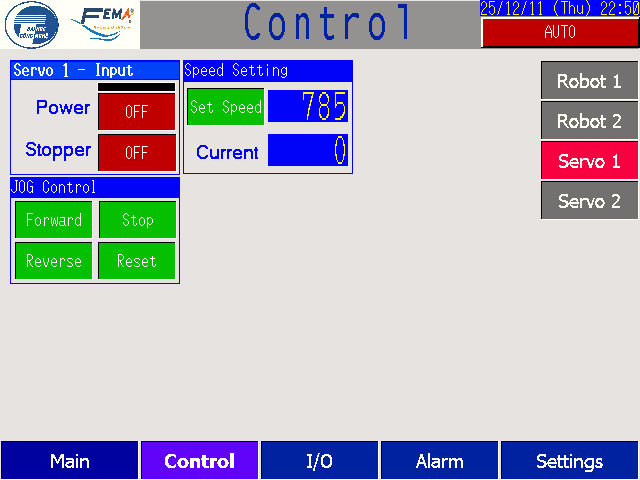
\includegraphics[width=0.48\linewidth]{figures/Chapter4/img4.jpg}
    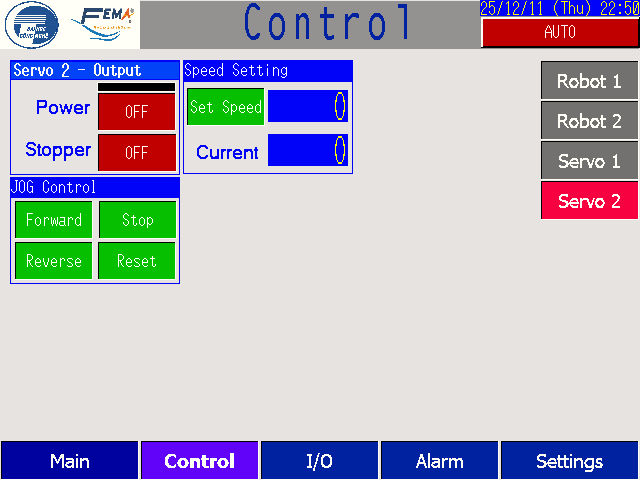
\includegraphics[width=0.48\linewidth]{figures/Chapter4/img5.jpg}
    \caption{Giao diện điều khiển Manual từng thành phần}
\end{figure}

\begin{figure}[H]
    \centering
    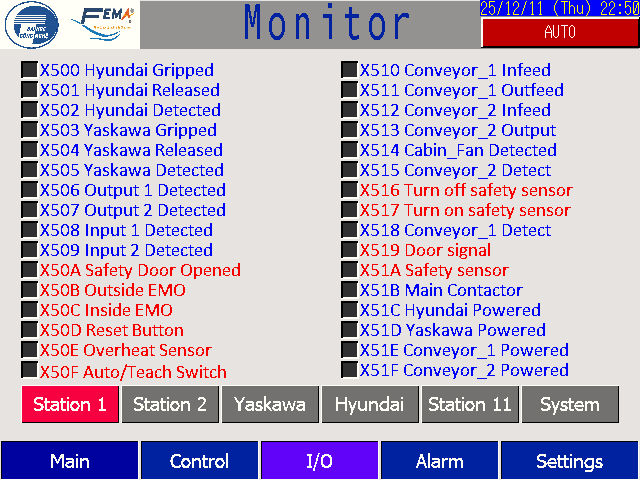
\includegraphics[width=0.48\linewidth]{figures/Chapter4/img6.jpg}
    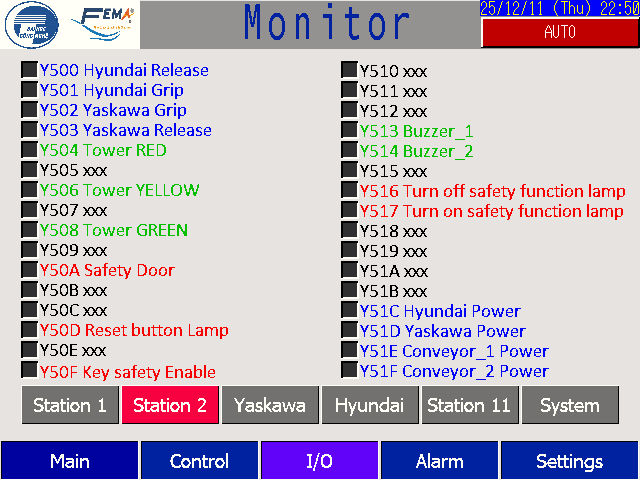
\includegraphics[width=0.48\linewidth]{figures/Chapter4/img7.jpg}
    \caption{Input/Output của hệ thống}
\end{figure}



\subsection{Kết quả nhận diện và phân loại sản phẩm}

Hình ảnh hệ thống sau khi lắp đặt:
\begin{figure}[H]
    \centering
    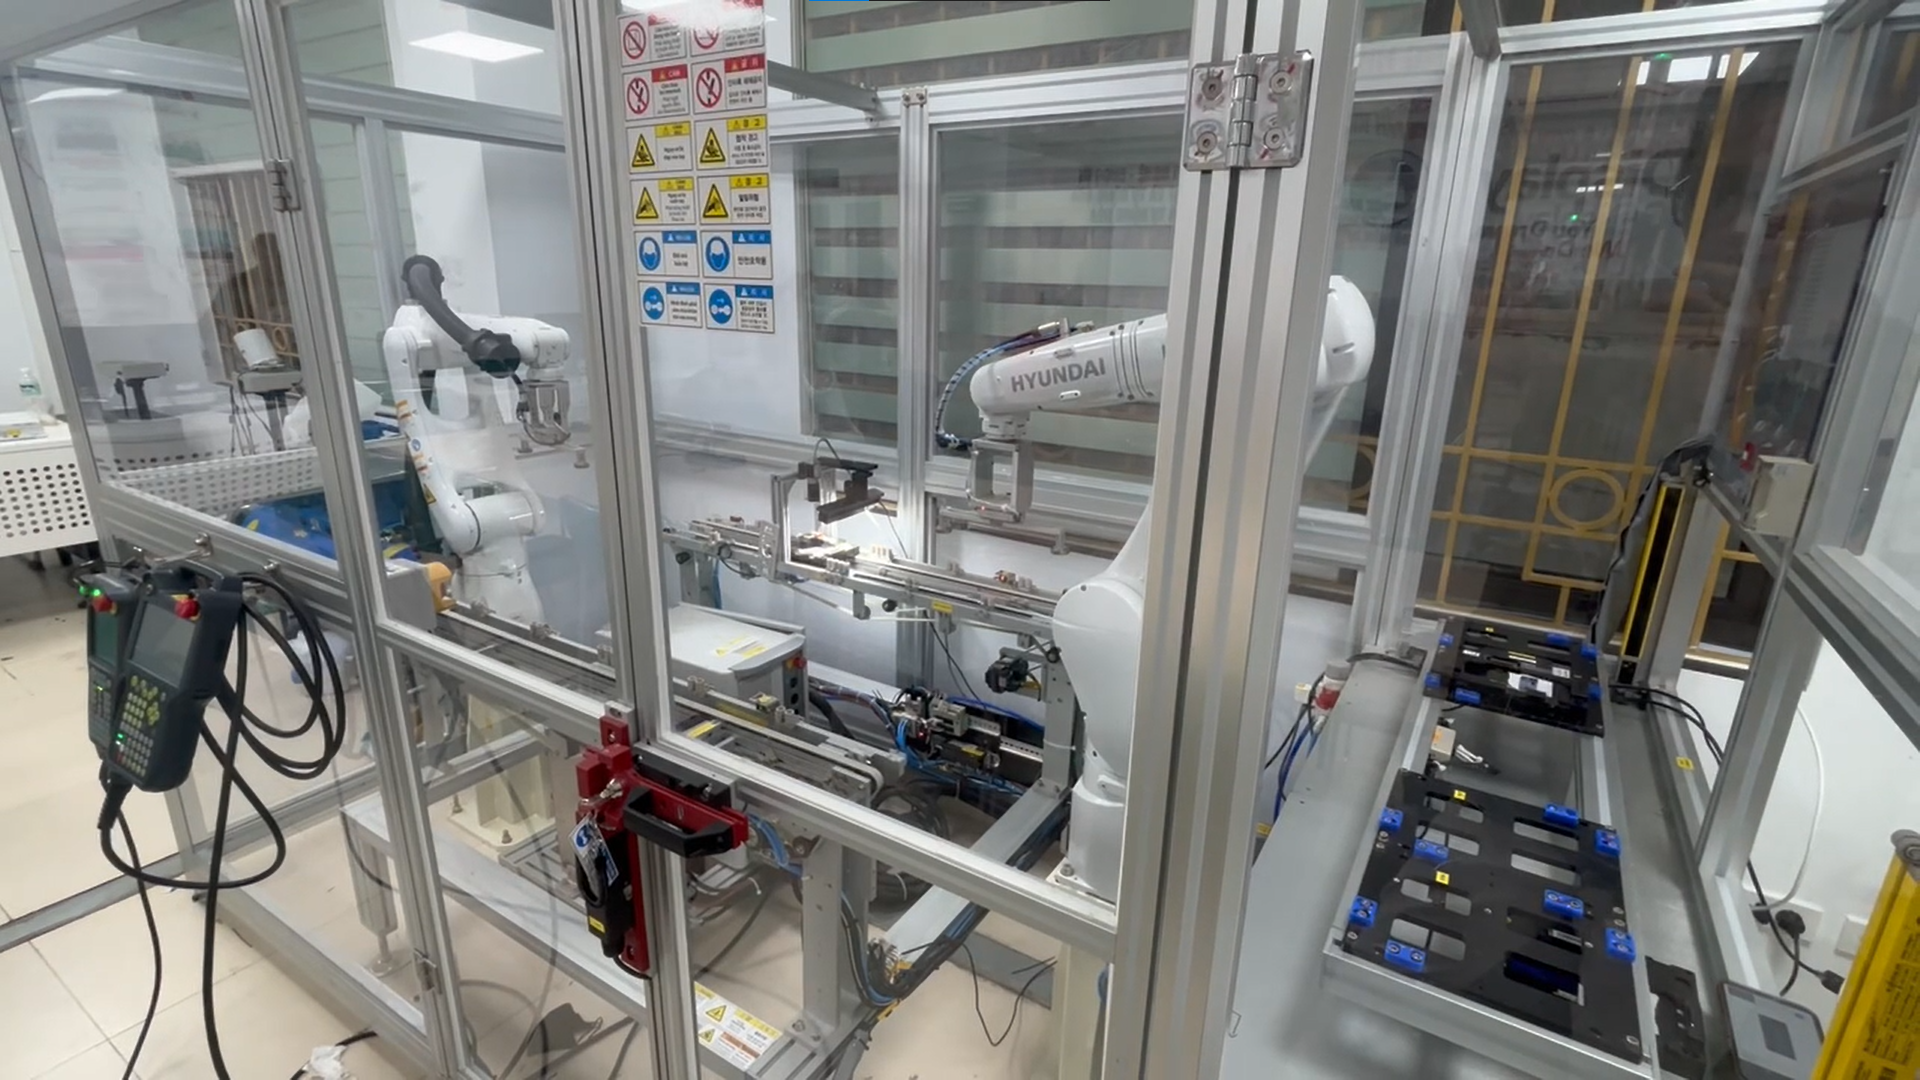
\includegraphics[width=1\linewidth]{figures/Chapter4/kq.png}
    \caption{Hệ thống thực tế}
\end{figure}

Hình ảnh giao diện ứng dụng khi hệ thống hoạt động:
\begin{figure}[H]
    \centering
    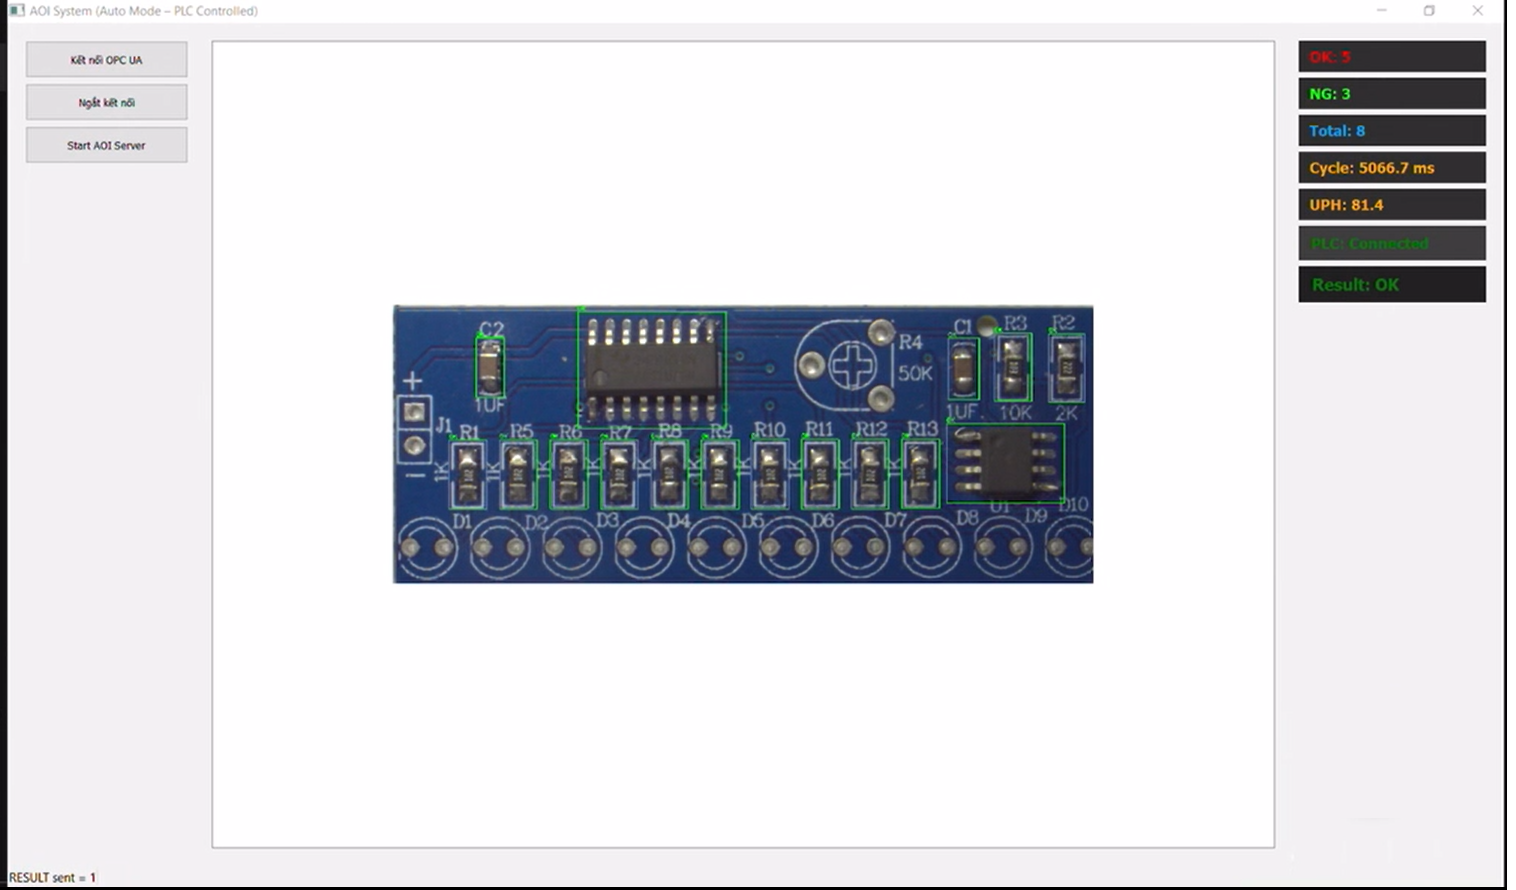
\includegraphics[width=1\linewidth]{figures/Chapter4/kq2.png}
    \caption{Kết quả hiển thị trên ứng dụng}
\end{figure}


Các thí nghiệm được thực hiện trên nhiều mẫu PCB bao gồm sản phẩm tốt và sản phẩm lỗi. Mô hình YOLO cho thấy khả năng nhận diện linh kiện SMD với độ chính xác cao, xác định đúng vị trí và loại linh kiện. Hệ thống phát hiện tốt các dạng lỗi phổ biến như thiếu linh kiện, lệch vị trí, xoay sai hướng và linh kiện sai loại. Các ảnh kết quả minh họa rõ vùng lỗi và hỗ trợ quá trình đánh giá sản phẩm.
Minh họa kết quả xử lý ảnh:
\begin{figure}[H]
    \centering
    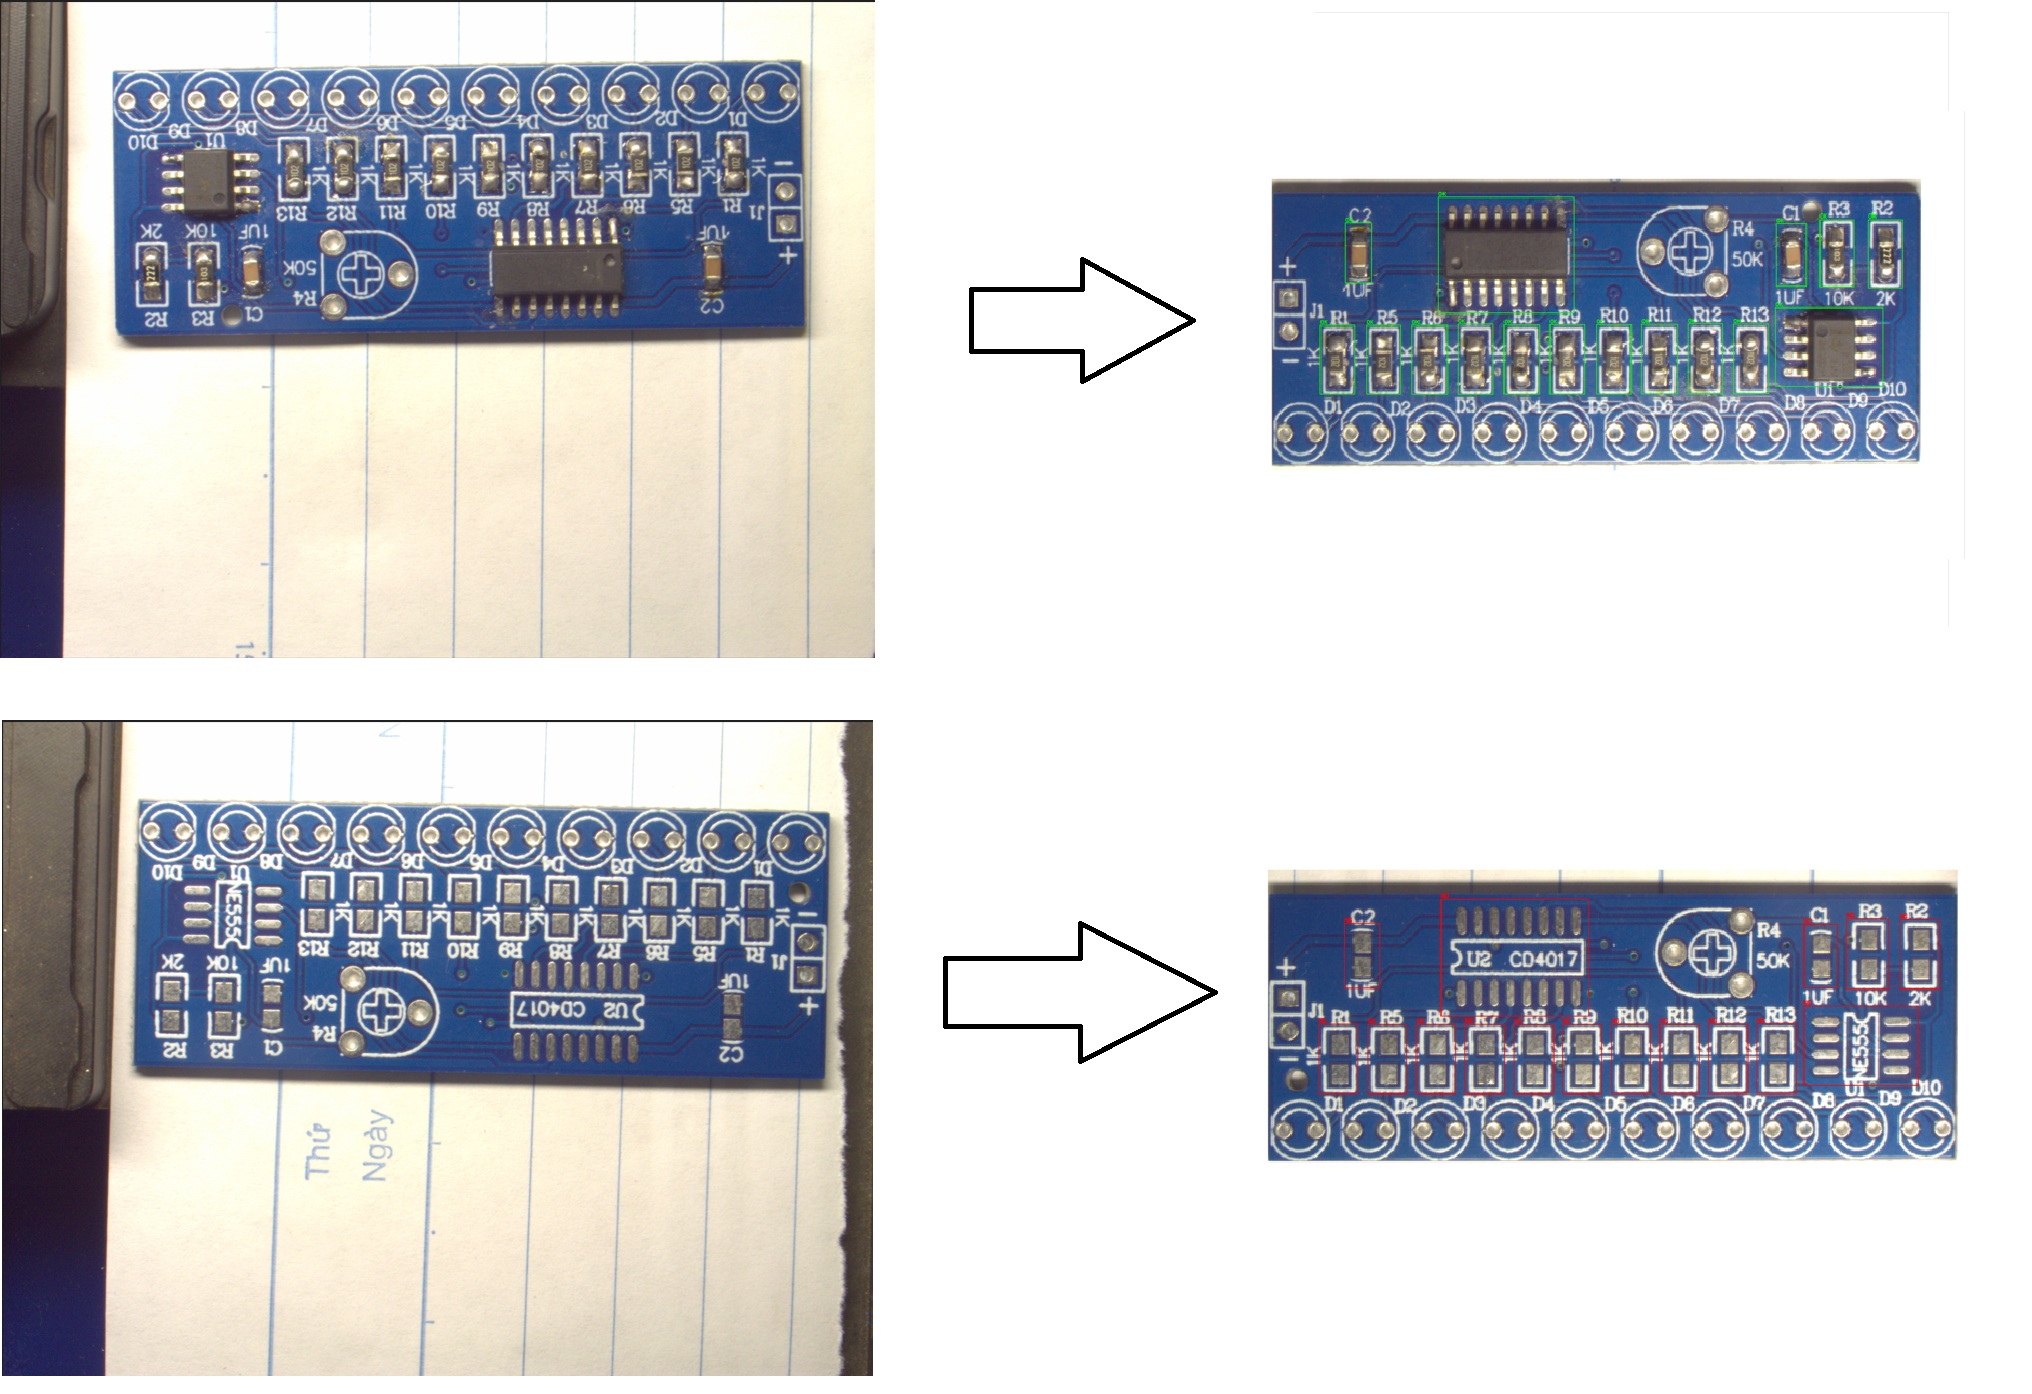
\includegraphics[width=1\linewidth]{figures/Chapter4/image3.png}
    \caption{Kết quả xử lý ảnh}
    \label{c4:image3}
\end{figure}


\subsection{Đánh giá hiệu suất: tốc độ, độ chính xác, độ ổn định}

Tốc độ xử lý trung bình của hệ thống đạt khoảng 3000--4000\,ms cho mỗi PCB, phụ thuộc nhiều vào phần cứng máy tính, đáp ứng tốt yêu cầu của dây chuyền sản xuất tốc độ cao. Độ chính xác nhận diện của mô hình YOLO đạt từ 95\% đến 98\%, trong khi các lỗi thiếu linh kiện được phát hiện với tỷ lệ 100\% Trong quá trình chạy liên tục nhiều giờ, hệ thống cho thấy tính ổn định cao, không phát sinh lỗi kết nối camera hoặc OPC UA.

\subsection{So sánh với phương pháp thủ công}

So với phương pháp kiểm tra thủ công bằng mắt thường, hệ thống AVI thể hiện ưu thế rõ rệt về tốc độ, độ chính xác và tính ổn định, đặc biệt khi sản phẩm cần kiểm tra có rất nhiều linh kiện nhỏ. Việc kiểm tra tự động giúp loại bỏ các sai sót chủ quan của người vận hành và phát hiện được những lỗi rất nhỏ mà mắt thường khó quan sát. Ngoài ra, hệ thống còn lưu trữ toàn bộ dữ liệu kiểm tra, hỗ trợ truy vết trong quá trình sản xuất. Do đó, phương pháp thủ công chỉ phù hợp cho kiểm tra mẫu hoặc sản lượng thấp, trong khi AVI là giải pháp tối ưu cho sản xuất hàng loạt.

\subsection{Cải tiến và nâng cấp}

Sau quá trình thiết kế và triển khai hệ thống kiểm tra ảnh tự động (AVI), có thể đề xuất một số hướng cải tiến nhằm nâng cao khả năng phát hiện lỗi, độ tin cậy và tính linh hoạt của hệ thống trong môi trường sản xuất thực tế.

\textbf{Thứ nhất}, cần mở rộng khả năng phát hiện nhiều loại lỗi hơn. Hệ thống hiện tại chủ yếu phát hiện các lỗi như thiếu linh kiện, lệch vị trí, xoay sai hướng và sai loại linh kiện. Để tăng cường hiệu quả kiểm tra, có thể bổ sung các lỗi nâng cao như dư linh kiện (gắn thừa), lệch quá giới hạn cho phép, sai giá trị linh kiện (ví dụ nhầm điện trở 1k và 10k), hoặc ngược cực linh kiện phân cực. Các lỗi này có thể được phát hiện bằng cách kết hợp kết quả từ mô hình YOLO với các thuật toán đo sai số hình học, phân loại patch bằng mạng CNN nhỏ, hoặc kiểm tra logic số lượng so với dữ liệu mẫu.

\textbf{Thứ hai}, hệ thống có thể được nâng cấp để hỗ trợ kiểm tra đa góc nhìn (6 sides inspection). Thay vì chỉ sử dụng ảnh chụp từ mặt trên (top view), có thể tích hợp thêm các camera ở cạnh bên hoặc góc nghiêng nhằm kiểm tra các mặt hông của linh kiện và bảng mạch. Phương pháp này giúp phát hiện các lỗi như thiếu chân IC, hàn dính cạnh, tụ bị ngẩng mặt (headstand), hoặc lỗi cơ khí mà ảnh mặt trên không thể quan sát được. Việc xử lý ảnh từ nhiều góc nhìn có thể được thực hiện bằng cách huấn luyện các mô hình riêng biệt cho từng camera hoặc sử dụng kỹ thuật căn chỉnh ảnh (warp perspective) trước khi xử lý.

\textbf{Thứ ba}, cần tích hợp thêm phương pháp phát hiện bất thường (anomaly detection) để xử lý các lỗi không lường trước hoặc không có sẵn nhãn huấn luyện. Trong môi trường sản xuất đa dạng, không thể liệt kê hết mọi dạng lỗi, đặc biệt là các lỗi hiếm. Do đó, sử dụng các mô hình học không giám sát như Autoencoder, PatchCore, hoặc PaDiM có thể giúp phát hiện các điểm bất thường dựa trên sai lệch phân phối đặc trưng so với mẫu chuẩn. Các kỹ thuật này có thể tạo ra bản đồ nhiệt (heatmap) vùng lỗi, giúp người vận hành nhận diện và đánh giá nguyên nhân nhanh chóng.

\textbf{Thứ tư}, giao diện người dùng (GUI) có thể được mở rộng để hỗ trợ các chức năng nâng cao như hiển thị phân tích lỗi theo thời gian thực, cho phép người dùng chọn chế độ kiểm tra (YOLO hoặc anomaly), truy xuất lại ảnh lỗi, và tự động lưu log kiểm tra theo batch sản xuất. Điều này không chỉ nâng cao trải nghiệm vận hành mà còn hỗ trợ quá trình truy vết và cải tiến chất lượng.

Tổng thể, các cải tiến trên góp phần nâng cao khả năng phát hiện lỗi toàn diện, tăng độ tin cậy của hệ thống trong các tình huống phức tạp, đồng thời tạo nền tảng để phát triển một hệ thống AVI linh hoạt, thông minh và có khả năng mở rộng trong tương lai.





\chapter*{KẾT LUẬN}
\addcontentsline{toc}{chapter}{{\bf KẾT LUẬN}}

Trong luận văn này, một hệ thống kiểm tra ngoại quan tự động (AVI) dựa trên thị giác máy tính đã được xây dựng và triển khai nhằm thay thế phương pháp kiểm tra thủ công trên dây chuyền sản xuất PCB. Hệ thống tích hợp đồng thời các thành phần phần cứng (camera công nghiệp, PLC Mitsubishi, robot Yaskawa và Hyundai, băng tải) và phần mềm (xử lý ảnh, mô hình học sâu YOLO, giao tiếp OPC UA), đáp ứng yêu cầu thực tế của quá trình sản xuất.

Về mặt thuật toán, luận văn đã đề xuất chuỗi xử lý ảnh theo dạng pipeline bao gồm các bước: thu nhận ảnh, tiền xử lý bằng CLAHE, căn chỉnh ảnh sử dụng đặc trưng ORB, cắt ROI dựa trên tọa độ chuẩn, phát hiện lỗi bằng mô hình YOLO và đánh giá sai lệch vị trí – góc xoay của linh kiện. Kết quả thực nghiệm cho thấy pipeline hoạt động ổn định, có khả năng mở rộng và phù hợp với môi trường sản xuất thực tế.

Về hiệu quả nhận diện, mô hình YOLO sau khi huấn luyện đã đạt độ chính xác từ 95\% đến 98\% tuỳ loại linh kiện và dạng lỗi. Thuật toán kiểm tra sai lệch dựa trên đối sánh đặc trưng cho phép xác định sai số vị trí và góc xoay với độ ổn định cao. Hệ thống phát hiện tốt các lỗi phổ biến như thiếu linh kiện, lệch vị trí, xoay sai hướng và sai loại, đáp ứng các tiêu chí chất lượng sản phẩm trong công nghiệp điện tử.

Về hiệu suất, thời gian xử lý trung bình đạt 800-1000\,ms cho mỗi PCB, phù hợp với dây chuyền tốc độ cao. Thử nghiệm chạy liên tục cho thấy hệ thống hoạt động ổn định, không xuất hiện lỗi kết nối camera, OPC UA hay robot, đảm bảo yêu cầu về độ tin cậy và vận hành lâu dài.

Kết quả so sánh với phương pháp kiểm tra thủ công cho thấy hệ thống AVI mang lại nhiều ưu điểm vượt trội: tốc độ nhanh hơn, loại bỏ sai sót do con người, phát hiện được lỗi tinh vi, đồng thời hỗ trợ lưu trữ và truy vết dữ liệu. Điều này khẳng định tính cần thiết và khả năng ứng dụng thực tiễn của hệ thống trong các dây chuyền sản xuất điện tử hiện đại.

Tóm lại, luận văn đã hoàn thành mục tiêu đề ra: xây dựng một hệ thống kiểm tra ngoại quan tự động dựa trên thị giác máy tính, ứng dụng mô hình học sâu và các thuật toán xử lý ảnh hiện đại, đồng thời tích hợp thành công với hệ thống điều khiển công nghiệp thực tế.

		
\include{tex/06congbo}	

\VKngatTrang
\VKtaiLieuThamKhao

\VKngatTrang
\VKdanhSoPhuLuc			

\titleformat{\chapter}{\bfseries \large \center}{PHỤ LỤC}{0.3em}{}[]

%\addcontentsline{toc}{chapter}{{\bf PHỤ LỤC}}
\thispagestyle{empty}

\appendix

\chapter[]{\\MỘT SỐ ĐOẠN MÃ NGUỒN} \label{manguon}

\section{Mã nguồn chụp ảnh bằng Camera Basler}
\label{sec:capture}
\lstinputlisting{code/pypylon.py}

\section{Mã nguồn xử lý tương phản bằng CLAHE}
\label{sec:clahe}
\lstinputlisting{code/clahe.py}
\VKngatTrang

\section{Mã nguồn xử lý ORB}
\label{sec:orb}
\lstinputlisting{code/orb.py}
\VKngatTrang

\end{document}



